% Capitolul 3: Rădăcini unitare și modele ARIMA
% Serii de timp -- Programele de licență Informatică economică și Cibernetică economică, Academia de Studii Economice din București
% GENERAT de latex/build_chapter3.py -- modificați generatorul, nu acest fișier.

\newcommand{\coursename}{Serii de timp}
\def\tsalang{ro}
% Preambul comun TSA -- Serii de timp / Time Series Analysis (Beamer, 16:9)
% Același design ca MFM și SFM (preluat din SFM, 5 octombrie 2026). Înainte de % Preambul comun TSA -- Serii de timp / Time Series Analysis (Beamer, 16:9)
% Același design ca MFM și SFM (preluat din SFM, 5 octombrie 2026). Înainte de % Preambul comun TSA -- Serii de timp / Time Series Analysis (Beamer, 16:9)
% Același design ca MFM și SFM (preluat din SFM, 5 octombrie 2026). Înainte de \input{../../latex/preamble} se definește
%   \newcommand{\coursename}{Time Series Analysis}      (EN)
%   \newcommand{\coursename}{Serii de timp}       (RO)  și  \def\tsalang{ro}
% Fișierele .tex se află în EN/Courses, EN/Seminars, RO/Cursuri, RO/Seminarii (două niveluri sub rădăcină).
% Deck-urile sînt generate de latex/build_chapterN.py / build_seminarN.py (vezi latex/tsa_build.py).

\documentclass[9pt, aspectratio=169, t]{beamer}
\providecommand{\coursename}{Time Series Analysis}

% Ensure content fits on slides
\setbeamersize{text margin left=8mm, text margin right=8mm}
% Smaller institute font (title page)
\setbeamerfont{institute}{size=\footnotesize}

%=============================================================================
% THEME AND STYLE CONFIGURATION
%=============================================================================
\usetheme{default}
% Using default theme for clean header/footer control

% Color Palette (matching Redispatch PDF)
\definecolor{MainBlue}{RGB}{26, 58, 110}
\definecolor{AccentBlue}{RGB}{26, 58, 110}
\definecolor{IDAred}{RGB}{205, 0, 0}
\definecolor{DarkGray}{RGB}{51, 51, 51}
\definecolor{MediumGray}{RGB}{128, 128, 128}
\definecolor{LightGray}{RGB}{248, 248, 248}
\definecolor{VeryLightGray}{RGB}{235, 235, 235}
\definecolor{KeynoteGray}{RGB}{218, 218, 218}
\definecolor{SectionGray}{RGB}{120, 120, 120}
\definecolor{FooterGray}{RGB}{100, 100, 100}
\definecolor{Crimson}{RGB}{220, 53, 69}
\definecolor{Forest}{RGB}{46, 125, 50}
\definecolor{Amber}{RGB}{181, 133, 63}
\definecolor{Orange}{RGB}{230, 126, 34}
\definecolor{Purple}{RGB}{142, 68, 173}

% Gradient background (exact Keynote 315° gradient: white to RGB 218,218,218)
\setbeamertemplate{background}{%
    \begin{tikzpicture}[remember picture, overlay]
        \shade[shading=axis, shading angle=315,
        top color=white, bottom color=KeynoteGray]
        (current page.south west) rectangle (current page.north east);
    \end{tikzpicture}%
}
% Fallback solid color for compatibility
\setbeamercolor{background canvas}{bg=}

\setbeamercolor{palette primary}{bg=MainBlue, fg=white}
\setbeamercolor{palette secondary}{bg=MainBlue!85, fg=white}
\setbeamercolor{palette tertiary}{bg=MainBlue!70, fg=white}
\setbeamercolor{structure}{fg=MainBlue}
\setbeamercolor{title}{fg=IDAred}
\setbeamercolor{frametitle}{fg=IDAred, bg=}
\setbeamercolor{block title}{bg=MainBlue, fg=white}
\setbeamercolor{block body}{bg=VeryLightGray, fg=DarkGray}
\setbeamercolor{block title alerted}{bg=Crimson, fg=white}
\setbeamercolor{block body alerted}{bg=Crimson!8, fg=DarkGray}
\setbeamercolor{block title example}{bg=Forest, fg=white}
\setbeamercolor{block body example}{bg=Forest!8, fg=DarkGray}
\setbeamercolor{item}{fg=MainBlue}

% Footer colors (override Madrid theme blue)
\setbeamercolor{author in head/foot}{fg=FooterGray, bg=}
\setbeamercolor{title in head/foot}{fg=FooterGray, bg=}
\setbeamercolor{date in head/foot}{fg=FooterGray, bg=}
\setbeamercolor{section in head/foot}{fg=FooterGray, bg=}
\setbeamercolor{subsection in head/foot}{fg=FooterGray, bg=}

% Bullet styles (apply everywhere including blocks)
\setbeamertemplate{itemize item}{\color{MainBlue}$\boxdot$}
\setbeamertemplate{itemize subitem}{\color{MainBlue}$\blacktriangleright$}
\setbeamertemplate{itemize subsubitem}{\color{MainBlue}\tiny$\bullet$}
\setbeamertemplate{itemize/enumerate body begin}{\normalsize}
\setbeamertemplate{itemize/enumerate subbody begin}{\normalsize}

% Item spacing - compact style
\setlength{\leftmargini}{10pt}       % Level 1: minimal indent
\setlength{\leftmarginii}{10pt}      % Level 2: minimal additional indent
% Compact list spacing (zero extra space before/after lists in blocks)
\makeatletter
\def\@listi{\leftmargin\leftmargini \topsep 0pt \parsep 0pt \itemsep 0pt}
\def\@listii{\leftmargin\leftmarginii \topsep 0pt \parsep 0pt \itemsep 0pt}
\makeatother

\setbeamertemplate{navigation symbols}{}

%=============================================================================
% CUSTOM HEADLINE
%=============================================================================
\setbeamertemplate{headline}{%
    \vskip10pt%
    \hbox to \paperwidth{%
        \hskip0.5cm%
        {\small\color{FooterGray}\renewcommand{\hyperlink}[2]{##2}\insertsectionhead}%
        \hfill%
        \textcolor{FooterGray}{\small\insertframenumber}%
        \hskip0.5cm%
    }%
    \vskip4pt%
    {\color{FooterGray}\hrule height 0.4pt}%
}

%=============================================================================
% CUSTOM FOOTER
%=============================================================================
\usepackage{fontawesome5}

\setbeamertemplate{footline}{%
    {\color{FooterGray}\hrule height 0.4pt}%
    \vskip4pt%
    \hbox to \paperwidth{%
        \hskip0.5cm%
        \textcolor{FooterGray}{\small\coursename}%
        \hfill%
        \raisebox{-0.1em}{%
            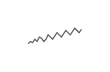
\begin{tikzpicture}[x=0.08em, y=0.08em, line width=0.4pt]
                \draw[FooterGray] (0,3) -- (1,4) -- (2,3.5) -- (3,5) -- (4,4) -- (5,6) -- (6,5.5) -- (7,4) -- (8,5) -- (9,7) -- (10,6) -- (11,5) -- (12,6.5) -- (13,8) -- (14,7) -- (15,6) -- (16,7.5) -- (17,9) -- (18,8) -- (19,7) -- (20,8.5) -- (21,10) -- (22,9) -- (23,8) -- (24,9.5);
            \end{tikzpicture}%
        }%
        \hskip0.5cm%
    }%
    \vskip6pt%
}

%=============================================================================
% PACKAGES
%=============================================================================
\usepackage[utf8]{inputenc}
\DeclareUnicodeCharacter{03B1}{\ensuremath{\alpha}}
\usepackage[T1]{fontenc}
\usepackage{amsmath, amssymb, amsthm}
\usepackage{mathtools}
\usepackage{bm}
\usepackage{tikz}
\usetikzlibrary{arrows.meta, positioning, shapes, calc, decorations.pathreplacing, shadings}
\usepackage{booktabs}
\usepackage{multirow}
\usepackage{array}
\usepackage{graphicx}
\usepackage{animate}
\usepackage{hyperref}
\usepackage{colortbl}
\usepackage{listings}
\lstset{language=Python, basicstyle=\ttfamily\scriptsize, keywordstyle=\color{MainBlue}\bfseries,
  commentstyle=\color{Forest}, stringstyle=\color{Crimson}, breaklines=true,
  frame=none, backgroundcolor=\color{VeryLightGray}, xleftmargin=2mm}
\hypersetup{colorlinks=true, linkcolor=MainBlue, urlcolor=MainBlue}
\graphicspath{{../../logos/}{../../charts/}{../../photos/}}
\usepackage{xcolor}
\hfuzz=2pt  % Suppress tiny overfull warnings (<2pt)
\vfuzz=2pt  % Suppress tiny vertical overfull warnings (<2pt)
% \mathrm in the sans-serif family of the slides (beamer resets \mathrm to the serif family at \begin{document};
% this hook runs after beamer's, so WN, Var, RMSE, ... in formulas match the surrounding text)
% Bold vectors and matrices in the same sans-serif family: \mathbf{A} in sans bold (beamer's own \mathbf came out in
% medium weight), and the bold upright Greek capitals of \boldsymbol / \bm (\bSigma, \bPhi, \boldsymbol{\Theta}) in
% cmss bold: bm.sty fixes its "boldoperators" font when it is loaded (serif cmbx), before beamer switches the
% operators to cmss, so it is reset here.
\AtBeginDocument{%
  \SetMathAlphabet{\mathrm}{normal}{\encodingdefault}{\sfdefault}{\mddefault}{n}%
  \SetMathAlphabet{\mathrm}{bold}{\encodingdefault}{\sfdefault}{bx}{n}%
  \SetMathAlphabet{\mathbf}{normal}{\encodingdefault}{\sfdefault}{bx}{n}%
  \SetMathAlphabet{\mathbf}{bold}{\encodingdefault}{\sfdefault}{bx}{n}%
  \SetSymbolFont{boldoperators}{normal}{OT1}{cmss}{bx}{n}%
  \SetSymbolFont{boldoperators}{bold}{OT1}{cmss}{bx}{n}}

%=============================================================================
% QUANTLET COMMANDS
%   \quantlet{<displayed name>}{<url>}       (generic, compatible with the older TSA decks)
%   \tsaquantlet{Ch_05}{TSA_ch5_garch}       -> https://github.com/danpele/Time-Series-Analysis/tree/main/Quantlets/Ch_05/TSA_ch5_garch
%   \qlurl{<folder>} is defined per chapter by the generator (Quantlets/Ch_NN/<folder>)
%=============================================================================
\newcommand{\tsarepo}{https://github.com/danpele/Time-Series-Analysis}
\newcommand{\tsaqlbase}{https://github.com/danpele/Time-Series-Analysis/tree/main/Quantlets}
\newcommand{\quantlet}[2]{%
    \hfill\href{#2}{%
        \raisebox{-0.15em}{
\includegraphics[height=0.7em]{ql_logo.png}}%
        \textcolor{MainBlue}{\tiny\ #1}%
    }%
}
\newcommand{\tsaquantlet}[2]{\quantlet{\detokenize{#2}}{\tsaqlbase/#1/#2}}

%=============================================================================
% NOTEBOOKS (Google Colab)
%   \colaburl{notebooks/EN/chapter5_seminar_notebook.ipynb} -> the Colab link of a file in the TSA repo
%   \nb: the chapter notebook (each seminar deck redefines it with \renewcommand)
%=============================================================================
\newcommand{\colaburl}[1]{https://colab.research.google.com/github/danpele/Time-Series-Analysis/blob/main/#1}
\newcommand{\nb}{https://colab.research.google.com/github/danpele/Time-Series-Analysis/tree/main/notebooks/EN}
\newcommand{\nbname}{notebooks/EN}

%=============================================================================
% SLIDE HELPERS (used by the generators; the same as in MFM)
%=============================================================================
% local font size for list bodies (the preamble forces \normalsize)
\newcommand{\itemsize}[1]{\setbeamertemplate{itemize/enumerate body begin}{#1}\setbeamertemplate{itemize/enumerate subbody begin}{#1}}
\newcommand{\intitle}[1]{{\hypersetup{urlcolor=white}#1}}   % white links inside coloured title bars
\newcommand{\imgcap}[1]{{\scriptsize #1}\\[0.5mm]}          % caption under a photo
\newcommand{\imgcredit}[2]{{\tiny\color{FooterGray}\href{#1}{#2}}}   % image credit: source URL, author/licence
\newcommand{\aiprompt}[1]{{\ttfamily\color{MainBlue}#1}}     % a prompt to an AI assistant

%=============================================================================
% SEMINARS: student version by default; the instructor wrapper *_solutions.tex sets \solutionstrue
%=============================================================================
\makeatletter\@ifundefined{ifsolutions}{\expandafter\newif\csname ifsolutions\endcsname}{}\makeatother
\newcommand{\solonly}[1]{\ifsolutions #1\fi}
\newcommand{\propsub}{\ifsolutions\else\framesubtitle{\ifdefined\tsalang Rezolvarea se discută la seminar\else Solution discussed in class\fi}\fi}

%=============================================================================
% APPENDIX AND CHAPTER LINKS (latex/appendix_links.py writes the calls; it also re-declares these
% macros before \begin{document}, so the decks compile with or without this preamble block)
%=============================================================================
\providecommand{\tsaapplink}[3]{\hypertarget{#2}{}\hyperlink{#1}{\beamergotobutton{#3}}}
\providecommand{\tsaappback}[2]{\begin{tikzpicture}[remember picture,overlay]\node[anchor=south east] at ([xshift=-3mm,yshift=7mm]current page.south east){\hyperlink{#1}{\beamerreturnbutton{#2}}};\end{tikzpicture}}
\providecommand{\tsachlink}[2]{\href{#1}{#2}}
\providecommand{\tsachlinkt}[2]{\href{#1}{\usebeamercolor[fg]{frametitle}#2}}

%=============================================================================
% QUANTINAR COMMAND: link către un curs Quantinar (subiecte avansate)
%=============================================================================
\newcommand{\quantinar}[2]{%
    \href{#2}{%
        \raisebox{-0.15em}{
\includegraphics[height=0.8em]{qr_logo.png}}%
        \textcolor{MainBlue}{\scriptsize\ #1}%
    }%
}

%=============================================================================
% CUSTOM TITLE PAGE
%=============================================================================
\defbeamertemplate*{title page}{hybrid}[1][]
{
    \vspace{0.2cm}
    % Logos row - top header (with clickable links)
    \begin{center}
        \href{https://www.ase.ro}{
\includegraphics[height=1.0cm]{ase_logo.png}}\hspace{0.3cm}%
        \href{https://theida.net}{
\includegraphics[height=1.0cm]{ida_logo.png}}\hspace{0.3cm}%
        \href{https://blockchain-research-center.com}{
\includegraphics[height=1.0cm]{brc_logo.png}}\hspace{0.3cm}%
        \href{https://www.ai4efin.ase.ro}{
\includegraphics[height=1.0cm]{ai4efin_logo.png}}\hspace{0.3cm}%
        \href{https://ipe.ro/new}{
\includegraphics[height=1.0cm]{acad_logo.png}}\hspace{0.3cm}%
        \href{https://www.digital-finance-msca.com}{
\includegraphics[height=1.0cm]{msca_logo.png}}%
    \end{center}

    \vspace{0.6cm}

    % Main title with Q logos on sides (with clickable links)
    \begin{center}
        \begin{minipage}{0.1\textwidth}
            \centering
            \href{https://quantlet.com}{
\includegraphics[height=1.1cm]{ql_logo.png}}
        \end{minipage}%
        \begin{minipage}{0.78\textwidth}
            \centering
            {\LARGE\bfseries\usebeamercolor[fg]{title}\inserttitle}

            \vspace{0.3cm}

            {\usebeamerfont{subtitle}\usebeamercolor[fg]{title}\insertsubtitle}
        \end{minipage}%
        \begin{minipage}{0.1\textwidth}
            \centering
            \href{https://quantinar.com}{
\includegraphics[height=1.1cm]{qr_logo.png}}
        \end{minipage}
    \end{center}

    \vspace{0.6cm}

    % Authors (left aligned)
    \hspace{0.5cm}{\usebeamerfont{author}\insertauthor}

    \vspace{0.3cm}

    % Institute/Affiliations (left aligned)
    \hspace{0.5cm}\begin{minipage}[t]{0.9\textwidth}
        \raggedright\small\insertinstitute
    \end{minipage}
}

%=============================================================================
% THEOREM ENVIRONMENTS
%=============================================================================
\theoremstyle{definition}
\setbeamertemplate{theorems}[numbered]
\ifdefined\tsalang
\newtheorem{defn}{Definiție}
\newtheorem{thm}{Teoremă}
\newtheorem{prop}{Propoziție}
\newtheorem{rmk}{Observație}
\else
\newtheorem{defn}{Definition}
\newtheorem{thm}{Theorem}
\newtheorem{prop}{Proposition}
\newtheorem{rmk}{Remark}
\fi

%=============================================================================
% CENTRED MINIPAGE (no extra vertical space)
%=============================================================================
\newenvironment{cminipage}[1]{%
    \par\noindent\hfill\begin{minipage}{#1}\ignorespaces
}{%
    \end{minipage}\hfill\null\par
}

%=============================================================================
% CUSTOM COMMANDS
%=============================================================================
\newcommand{\E}{\mathbb{E}}
\newcommand{\Var}{\text{Var}}
\newcommand{\Cov}{\text{Cov}}
\newcommand{\Corr}{\text{Corr}}
\newcommand{\R}{\mathbb{R}}
\newcommand{\N}{\mathbb{N}}
\newcommand{\Z}{\mathbb{Z}}
\newcommand{\B}{\mathbf{B}}
\newcommand{\imark}{\textcolor{MainBlue}{\textbullet}}
\newcommand{\RMSE}{\text{RMSE}}
\newcommand{\MAE}{\text{MAE}}
\newcommand{\MAPE}{\text{MAPE}}

% Boldface vector/matrix commands (VAR, VECM, state space; also used by the older TSA decks)
\newcommand{\bY}{\mathbf{Y}}
\newcommand{\bX}{\mathbf{X}}
\newcommand{\bA}{\mathbf{A}}
\newcommand{\bB}{\mathbf{B}}
\newcommand{\bepsilon}{\boldsymbol{\varepsilon}}
\newcommand{\bSigma}{\boldsymbol{\Sigma}}
\newcommand{\bPhi}{\boldsymbol{\Phi}}
\newcommand{\bGamma}{\boldsymbol{\Gamma}}
\newcommand{\bPi}{\boldsymbol{\Pi}}
\newcommand{\bc}{\mathbf{c}}
\newcommand{\balpha}{\boldsymbol{\alpha}}
\newcommand{\bbeta}{\boldsymbol{\beta}}
\newcommand{\bvarepsilon}{\boldsymbol{\varepsilon}}

% Legacy seminar marks (older TSA seminar decks)
\newcommand{\correct}{\textcolor{Forest}{\checkmark}}
\newcommand{\incorrect}{\textcolor{Crimson}{\texttimes}}
 se definește
%   \newcommand{\coursename}{Time Series Analysis}      (EN)
%   \newcommand{\coursename}{Serii de timp}       (RO)  și  \def\tsalang{ro}
% Fișierele .tex se află în EN/Courses, EN/Seminars, RO/Cursuri, RO/Seminarii (două niveluri sub rădăcină).
% Deck-urile sînt generate de latex/build_chapterN.py / build_seminarN.py (vezi latex/tsa_build.py).

\documentclass[9pt, aspectratio=169, t]{beamer}
\providecommand{\coursename}{Time Series Analysis}

% Ensure content fits on slides
\setbeamersize{text margin left=8mm, text margin right=8mm}
% Smaller institute font (title page)
\setbeamerfont{institute}{size=\footnotesize}

%=============================================================================
% THEME AND STYLE CONFIGURATION
%=============================================================================
\usetheme{default}
% Using default theme for clean header/footer control

% Color Palette (matching Redispatch PDF)
\definecolor{MainBlue}{RGB}{26, 58, 110}
\definecolor{AccentBlue}{RGB}{26, 58, 110}
\definecolor{IDAred}{RGB}{205, 0, 0}
\definecolor{DarkGray}{RGB}{51, 51, 51}
\definecolor{MediumGray}{RGB}{128, 128, 128}
\definecolor{LightGray}{RGB}{248, 248, 248}
\definecolor{VeryLightGray}{RGB}{235, 235, 235}
\definecolor{KeynoteGray}{RGB}{218, 218, 218}
\definecolor{SectionGray}{RGB}{120, 120, 120}
\definecolor{FooterGray}{RGB}{100, 100, 100}
\definecolor{Crimson}{RGB}{220, 53, 69}
\definecolor{Forest}{RGB}{46, 125, 50}
\definecolor{Amber}{RGB}{181, 133, 63}
\definecolor{Orange}{RGB}{230, 126, 34}
\definecolor{Purple}{RGB}{142, 68, 173}

% Gradient background (exact Keynote 315° gradient: white to RGB 218,218,218)
\setbeamertemplate{background}{%
    \begin{tikzpicture}[remember picture, overlay]
        \shade[shading=axis, shading angle=315,
        top color=white, bottom color=KeynoteGray]
        (current page.south west) rectangle (current page.north east);
    \end{tikzpicture}%
}
% Fallback solid color for compatibility
\setbeamercolor{background canvas}{bg=}

\setbeamercolor{palette primary}{bg=MainBlue, fg=white}
\setbeamercolor{palette secondary}{bg=MainBlue!85, fg=white}
\setbeamercolor{palette tertiary}{bg=MainBlue!70, fg=white}
\setbeamercolor{structure}{fg=MainBlue}
\setbeamercolor{title}{fg=IDAred}
\setbeamercolor{frametitle}{fg=IDAred, bg=}
\setbeamercolor{block title}{bg=MainBlue, fg=white}
\setbeamercolor{block body}{bg=VeryLightGray, fg=DarkGray}
\setbeamercolor{block title alerted}{bg=Crimson, fg=white}
\setbeamercolor{block body alerted}{bg=Crimson!8, fg=DarkGray}
\setbeamercolor{block title example}{bg=Forest, fg=white}
\setbeamercolor{block body example}{bg=Forest!8, fg=DarkGray}
\setbeamercolor{item}{fg=MainBlue}

% Footer colors (override Madrid theme blue)
\setbeamercolor{author in head/foot}{fg=FooterGray, bg=}
\setbeamercolor{title in head/foot}{fg=FooterGray, bg=}
\setbeamercolor{date in head/foot}{fg=FooterGray, bg=}
\setbeamercolor{section in head/foot}{fg=FooterGray, bg=}
\setbeamercolor{subsection in head/foot}{fg=FooterGray, bg=}

% Bullet styles (apply everywhere including blocks)
\setbeamertemplate{itemize item}{\color{MainBlue}$\boxdot$}
\setbeamertemplate{itemize subitem}{\color{MainBlue}$\blacktriangleright$}
\setbeamertemplate{itemize subsubitem}{\color{MainBlue}\tiny$\bullet$}
\setbeamertemplate{itemize/enumerate body begin}{\normalsize}
\setbeamertemplate{itemize/enumerate subbody begin}{\normalsize}

% Item spacing - compact style
\setlength{\leftmargini}{10pt}       % Level 1: minimal indent
\setlength{\leftmarginii}{10pt}      % Level 2: minimal additional indent
% Compact list spacing (zero extra space before/after lists in blocks)
\makeatletter
\def\@listi{\leftmargin\leftmargini \topsep 0pt \parsep 0pt \itemsep 0pt}
\def\@listii{\leftmargin\leftmarginii \topsep 0pt \parsep 0pt \itemsep 0pt}
\makeatother

\setbeamertemplate{navigation symbols}{}

%=============================================================================
% CUSTOM HEADLINE
%=============================================================================
\setbeamertemplate{headline}{%
    \vskip10pt%
    \hbox to \paperwidth{%
        \hskip0.5cm%
        {\small\color{FooterGray}\renewcommand{\hyperlink}[2]{##2}\insertsectionhead}%
        \hfill%
        \textcolor{FooterGray}{\small\insertframenumber}%
        \hskip0.5cm%
    }%
    \vskip4pt%
    {\color{FooterGray}\hrule height 0.4pt}%
}

%=============================================================================
% CUSTOM FOOTER
%=============================================================================
\usepackage{fontawesome5}

\setbeamertemplate{footline}{%
    {\color{FooterGray}\hrule height 0.4pt}%
    \vskip4pt%
    \hbox to \paperwidth{%
        \hskip0.5cm%
        \textcolor{FooterGray}{\small\coursename}%
        \hfill%
        \raisebox{-0.1em}{%
            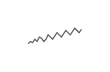
\begin{tikzpicture}[x=0.08em, y=0.08em, line width=0.4pt]
                \draw[FooterGray] (0,3) -- (1,4) -- (2,3.5) -- (3,5) -- (4,4) -- (5,6) -- (6,5.5) -- (7,4) -- (8,5) -- (9,7) -- (10,6) -- (11,5) -- (12,6.5) -- (13,8) -- (14,7) -- (15,6) -- (16,7.5) -- (17,9) -- (18,8) -- (19,7) -- (20,8.5) -- (21,10) -- (22,9) -- (23,8) -- (24,9.5);
            \end{tikzpicture}%
        }%
        \hskip0.5cm%
    }%
    \vskip6pt%
}

%=============================================================================
% PACKAGES
%=============================================================================
\usepackage[utf8]{inputenc}
\DeclareUnicodeCharacter{03B1}{\ensuremath{\alpha}}
\usepackage[T1]{fontenc}
\usepackage{amsmath, amssymb, amsthm}
\usepackage{mathtools}
\usepackage{bm}
\usepackage{tikz}
\usetikzlibrary{arrows.meta, positioning, shapes, calc, decorations.pathreplacing, shadings}
\usepackage{booktabs}
\usepackage{multirow}
\usepackage{array}
\usepackage{graphicx}
\usepackage{animate}
\usepackage{hyperref}
\usepackage{colortbl}
\usepackage{listings}
\lstset{language=Python, basicstyle=\ttfamily\scriptsize, keywordstyle=\color{MainBlue}\bfseries,
  commentstyle=\color{Forest}, stringstyle=\color{Crimson}, breaklines=true,
  frame=none, backgroundcolor=\color{VeryLightGray}, xleftmargin=2mm}
\hypersetup{colorlinks=true, linkcolor=MainBlue, urlcolor=MainBlue}
\graphicspath{{../../logos/}{../../charts/}{../../photos/}}
\usepackage{xcolor}
\hfuzz=2pt  % Suppress tiny overfull warnings (<2pt)
\vfuzz=2pt  % Suppress tiny vertical overfull warnings (<2pt)
% \mathrm in the sans-serif family of the slides (beamer resets \mathrm to the serif family at \begin{document};
% this hook runs after beamer's, so WN, Var, RMSE, ... in formulas match the surrounding text)
% Bold vectors and matrices in the same sans-serif family: \mathbf{A} in sans bold (beamer's own \mathbf came out in
% medium weight), and the bold upright Greek capitals of \boldsymbol / \bm (\bSigma, \bPhi, \boldsymbol{\Theta}) in
% cmss bold: bm.sty fixes its "boldoperators" font when it is loaded (serif cmbx), before beamer switches the
% operators to cmss, so it is reset here.
\AtBeginDocument{%
  \SetMathAlphabet{\mathrm}{normal}{\encodingdefault}{\sfdefault}{\mddefault}{n}%
  \SetMathAlphabet{\mathrm}{bold}{\encodingdefault}{\sfdefault}{bx}{n}%
  \SetMathAlphabet{\mathbf}{normal}{\encodingdefault}{\sfdefault}{bx}{n}%
  \SetMathAlphabet{\mathbf}{bold}{\encodingdefault}{\sfdefault}{bx}{n}%
  \SetSymbolFont{boldoperators}{normal}{OT1}{cmss}{bx}{n}%
  \SetSymbolFont{boldoperators}{bold}{OT1}{cmss}{bx}{n}}

%=============================================================================
% QUANTLET COMMANDS
%   \quantlet{<displayed name>}{<url>}       (generic, compatible with the older TSA decks)
%   \tsaquantlet{Ch_05}{TSA_ch5_garch}       -> https://github.com/danpele/Time-Series-Analysis/tree/main/Quantlets/Ch_05/TSA_ch5_garch
%   \qlurl{<folder>} is defined per chapter by the generator (Quantlets/Ch_NN/<folder>)
%=============================================================================
\newcommand{\tsarepo}{https://github.com/danpele/Time-Series-Analysis}
\newcommand{\tsaqlbase}{https://github.com/danpele/Time-Series-Analysis/tree/main/Quantlets}
\newcommand{\quantlet}[2]{%
    \hfill\href{#2}{%
        \raisebox{-0.15em}{
\includegraphics[height=0.7em]{ql_logo.png}}%
        \textcolor{MainBlue}{\tiny\ #1}%
    }%
}
\newcommand{\tsaquantlet}[2]{\quantlet{\detokenize{#2}}{\tsaqlbase/#1/#2}}

%=============================================================================
% NOTEBOOKS (Google Colab)
%   \colaburl{notebooks/EN/chapter5_seminar_notebook.ipynb} -> the Colab link of a file in the TSA repo
%   \nb: the chapter notebook (each seminar deck redefines it with \renewcommand)
%=============================================================================
\newcommand{\colaburl}[1]{https://colab.research.google.com/github/danpele/Time-Series-Analysis/blob/main/#1}
\newcommand{\nb}{https://colab.research.google.com/github/danpele/Time-Series-Analysis/tree/main/notebooks/EN}
\newcommand{\nbname}{notebooks/EN}

%=============================================================================
% SLIDE HELPERS (used by the generators; the same as in MFM)
%=============================================================================
% local font size for list bodies (the preamble forces \normalsize)
\newcommand{\itemsize}[1]{\setbeamertemplate{itemize/enumerate body begin}{#1}\setbeamertemplate{itemize/enumerate subbody begin}{#1}}
\newcommand{\intitle}[1]{{\hypersetup{urlcolor=white}#1}}   % white links inside coloured title bars
\newcommand{\imgcap}[1]{{\scriptsize #1}\\[0.5mm]}          % caption under a photo
\newcommand{\imgcredit}[2]{{\tiny\color{FooterGray}\href{#1}{#2}}}   % image credit: source URL, author/licence
\newcommand{\aiprompt}[1]{{\ttfamily\color{MainBlue}#1}}     % a prompt to an AI assistant

%=============================================================================
% SEMINARS: student version by default; the instructor wrapper *_solutions.tex sets \solutionstrue
%=============================================================================
\makeatletter\@ifundefined{ifsolutions}{\expandafter\newif\csname ifsolutions\endcsname}{}\makeatother
\newcommand{\solonly}[1]{\ifsolutions #1\fi}
\newcommand{\propsub}{\ifsolutions\else\framesubtitle{\ifdefined\tsalang Rezolvarea se discută la seminar\else Solution discussed in class\fi}\fi}

%=============================================================================
% APPENDIX AND CHAPTER LINKS (latex/appendix_links.py writes the calls; it also re-declares these
% macros before \begin{document}, so the decks compile with or without this preamble block)
%=============================================================================
\providecommand{\tsaapplink}[3]{\hypertarget{#2}{}\hyperlink{#1}{\beamergotobutton{#3}}}
\providecommand{\tsaappback}[2]{\begin{tikzpicture}[remember picture,overlay]\node[anchor=south east] at ([xshift=-3mm,yshift=7mm]current page.south east){\hyperlink{#1}{\beamerreturnbutton{#2}}};\end{tikzpicture}}
\providecommand{\tsachlink}[2]{\href{#1}{#2}}
\providecommand{\tsachlinkt}[2]{\href{#1}{\usebeamercolor[fg]{frametitle}#2}}

%=============================================================================
% QUANTINAR COMMAND: link către un curs Quantinar (subiecte avansate)
%=============================================================================
\newcommand{\quantinar}[2]{%
    \href{#2}{%
        \raisebox{-0.15em}{
\includegraphics[height=0.8em]{qr_logo.png}}%
        \textcolor{MainBlue}{\scriptsize\ #1}%
    }%
}

%=============================================================================
% CUSTOM TITLE PAGE
%=============================================================================
\defbeamertemplate*{title page}{hybrid}[1][]
{
    \vspace{0.2cm}
    % Logos row - top header (with clickable links)
    \begin{center}
        \href{https://www.ase.ro}{
\includegraphics[height=1.0cm]{ase_logo.png}}\hspace{0.3cm}%
        \href{https://theida.net}{
\includegraphics[height=1.0cm]{ida_logo.png}}\hspace{0.3cm}%
        \href{https://blockchain-research-center.com}{
\includegraphics[height=1.0cm]{brc_logo.png}}\hspace{0.3cm}%
        \href{https://www.ai4efin.ase.ro}{
\includegraphics[height=1.0cm]{ai4efin_logo.png}}\hspace{0.3cm}%
        \href{https://ipe.ro/new}{
\includegraphics[height=1.0cm]{acad_logo.png}}\hspace{0.3cm}%
        \href{https://www.digital-finance-msca.com}{
\includegraphics[height=1.0cm]{msca_logo.png}}%
    \end{center}

    \vspace{0.6cm}

    % Main title with Q logos on sides (with clickable links)
    \begin{center}
        \begin{minipage}{0.1\textwidth}
            \centering
            \href{https://quantlet.com}{
\includegraphics[height=1.1cm]{ql_logo.png}}
        \end{minipage}%
        \begin{minipage}{0.78\textwidth}
            \centering
            {\LARGE\bfseries\usebeamercolor[fg]{title}\inserttitle}

            \vspace{0.3cm}

            {\usebeamerfont{subtitle}\usebeamercolor[fg]{title}\insertsubtitle}
        \end{minipage}%
        \begin{minipage}{0.1\textwidth}
            \centering
            \href{https://quantinar.com}{
\includegraphics[height=1.1cm]{qr_logo.png}}
        \end{minipage}
    \end{center}

    \vspace{0.6cm}

    % Authors (left aligned)
    \hspace{0.5cm}{\usebeamerfont{author}\insertauthor}

    \vspace{0.3cm}

    % Institute/Affiliations (left aligned)
    \hspace{0.5cm}\begin{minipage}[t]{0.9\textwidth}
        \raggedright\small\insertinstitute
    \end{minipage}
}

%=============================================================================
% THEOREM ENVIRONMENTS
%=============================================================================
\theoremstyle{definition}
\setbeamertemplate{theorems}[numbered]
\ifdefined\tsalang
\newtheorem{defn}{Definiție}
\newtheorem{thm}{Teoremă}
\newtheorem{prop}{Propoziție}
\newtheorem{rmk}{Observație}
\else
\newtheorem{defn}{Definition}
\newtheorem{thm}{Theorem}
\newtheorem{prop}{Proposition}
\newtheorem{rmk}{Remark}
\fi

%=============================================================================
% CENTRED MINIPAGE (no extra vertical space)
%=============================================================================
\newenvironment{cminipage}[1]{%
    \par\noindent\hfill\begin{minipage}{#1}\ignorespaces
}{%
    \end{minipage}\hfill\null\par
}

%=============================================================================
% CUSTOM COMMANDS
%=============================================================================
\newcommand{\E}{\mathbb{E}}
\newcommand{\Var}{\text{Var}}
\newcommand{\Cov}{\text{Cov}}
\newcommand{\Corr}{\text{Corr}}
\newcommand{\R}{\mathbb{R}}
\newcommand{\N}{\mathbb{N}}
\newcommand{\Z}{\mathbb{Z}}
\newcommand{\B}{\mathbf{B}}
\newcommand{\imark}{\textcolor{MainBlue}{\textbullet}}
\newcommand{\RMSE}{\text{RMSE}}
\newcommand{\MAE}{\text{MAE}}
\newcommand{\MAPE}{\text{MAPE}}

% Boldface vector/matrix commands (VAR, VECM, state space; also used by the older TSA decks)
\newcommand{\bY}{\mathbf{Y}}
\newcommand{\bX}{\mathbf{X}}
\newcommand{\bA}{\mathbf{A}}
\newcommand{\bB}{\mathbf{B}}
\newcommand{\bepsilon}{\boldsymbol{\varepsilon}}
\newcommand{\bSigma}{\boldsymbol{\Sigma}}
\newcommand{\bPhi}{\boldsymbol{\Phi}}
\newcommand{\bGamma}{\boldsymbol{\Gamma}}
\newcommand{\bPi}{\boldsymbol{\Pi}}
\newcommand{\bc}{\mathbf{c}}
\newcommand{\balpha}{\boldsymbol{\alpha}}
\newcommand{\bbeta}{\boldsymbol{\beta}}
\newcommand{\bvarepsilon}{\boldsymbol{\varepsilon}}

% Legacy seminar marks (older TSA seminar decks)
\newcommand{\correct}{\textcolor{Forest}{\checkmark}}
\newcommand{\incorrect}{\textcolor{Crimson}{\texttimes}}
 se definește
%   \newcommand{\coursename}{Time Series Analysis}      (EN)
%   \newcommand{\coursename}{Serii de timp}       (RO)  și  \def\tsalang{ro}
% Fișierele .tex se află în EN/Courses, EN/Seminars, RO/Cursuri, RO/Seminarii (două niveluri sub rădăcină).
% Deck-urile sînt generate de latex/build_chapterN.py / build_seminarN.py (vezi latex/tsa_build.py).

\documentclass[9pt, aspectratio=169, t]{beamer}
\providecommand{\coursename}{Time Series Analysis}

% Ensure content fits on slides
\setbeamersize{text margin left=8mm, text margin right=8mm}
% Smaller institute font (title page)
\setbeamerfont{institute}{size=\footnotesize}

%=============================================================================
% THEME AND STYLE CONFIGURATION
%=============================================================================
\usetheme{default}
% Using default theme for clean header/footer control

% Color Palette (matching Redispatch PDF)
\definecolor{MainBlue}{RGB}{26, 58, 110}
\definecolor{AccentBlue}{RGB}{26, 58, 110}
\definecolor{IDAred}{RGB}{205, 0, 0}
\definecolor{DarkGray}{RGB}{51, 51, 51}
\definecolor{MediumGray}{RGB}{128, 128, 128}
\definecolor{LightGray}{RGB}{248, 248, 248}
\definecolor{VeryLightGray}{RGB}{235, 235, 235}
\definecolor{KeynoteGray}{RGB}{218, 218, 218}
\definecolor{SectionGray}{RGB}{120, 120, 120}
\definecolor{FooterGray}{RGB}{100, 100, 100}
\definecolor{Crimson}{RGB}{220, 53, 69}
\definecolor{Forest}{RGB}{46, 125, 50}
\definecolor{Amber}{RGB}{181, 133, 63}
\definecolor{Orange}{RGB}{230, 126, 34}
\definecolor{Purple}{RGB}{142, 68, 173}

% Gradient background (exact Keynote 315° gradient: white to RGB 218,218,218)
\setbeamertemplate{background}{%
    \begin{tikzpicture}[remember picture, overlay]
        \shade[shading=axis, shading angle=315,
        top color=white, bottom color=KeynoteGray]
        (current page.south west) rectangle (current page.north east);
    \end{tikzpicture}%
}
% Fallback solid color for compatibility
\setbeamercolor{background canvas}{bg=}

\setbeamercolor{palette primary}{bg=MainBlue, fg=white}
\setbeamercolor{palette secondary}{bg=MainBlue!85, fg=white}
\setbeamercolor{palette tertiary}{bg=MainBlue!70, fg=white}
\setbeamercolor{structure}{fg=MainBlue}
\setbeamercolor{title}{fg=IDAred}
\setbeamercolor{frametitle}{fg=IDAred, bg=}
\setbeamercolor{block title}{bg=MainBlue, fg=white}
\setbeamercolor{block body}{bg=VeryLightGray, fg=DarkGray}
\setbeamercolor{block title alerted}{bg=Crimson, fg=white}
\setbeamercolor{block body alerted}{bg=Crimson!8, fg=DarkGray}
\setbeamercolor{block title example}{bg=Forest, fg=white}
\setbeamercolor{block body example}{bg=Forest!8, fg=DarkGray}
\setbeamercolor{item}{fg=MainBlue}

% Footer colors (override Madrid theme blue)
\setbeamercolor{author in head/foot}{fg=FooterGray, bg=}
\setbeamercolor{title in head/foot}{fg=FooterGray, bg=}
\setbeamercolor{date in head/foot}{fg=FooterGray, bg=}
\setbeamercolor{section in head/foot}{fg=FooterGray, bg=}
\setbeamercolor{subsection in head/foot}{fg=FooterGray, bg=}

% Bullet styles (apply everywhere including blocks)
\setbeamertemplate{itemize item}{\color{MainBlue}$\boxdot$}
\setbeamertemplate{itemize subitem}{\color{MainBlue}$\blacktriangleright$}
\setbeamertemplate{itemize subsubitem}{\color{MainBlue}\tiny$\bullet$}
\setbeamertemplate{itemize/enumerate body begin}{\normalsize}
\setbeamertemplate{itemize/enumerate subbody begin}{\normalsize}

% Item spacing - compact style
\setlength{\leftmargini}{10pt}       % Level 1: minimal indent
\setlength{\leftmarginii}{10pt}      % Level 2: minimal additional indent
% Compact list spacing (zero extra space before/after lists in blocks)
\makeatletter
\def\@listi{\leftmargin\leftmargini \topsep 0pt \parsep 0pt \itemsep 0pt}
\def\@listii{\leftmargin\leftmarginii \topsep 0pt \parsep 0pt \itemsep 0pt}
\makeatother

\setbeamertemplate{navigation symbols}{}

%=============================================================================
% CUSTOM HEADLINE
%=============================================================================
\setbeamertemplate{headline}{%
    \vskip10pt%
    \hbox to \paperwidth{%
        \hskip0.5cm%
        {\small\color{FooterGray}\renewcommand{\hyperlink}[2]{##2}\insertsectionhead}%
        \hfill%
        \textcolor{FooterGray}{\small\insertframenumber}%
        \hskip0.5cm%
    }%
    \vskip4pt%
    {\color{FooterGray}\hrule height 0.4pt}%
}

%=============================================================================
% CUSTOM FOOTER
%=============================================================================
\usepackage{fontawesome5}

\setbeamertemplate{footline}{%
    {\color{FooterGray}\hrule height 0.4pt}%
    \vskip4pt%
    \hbox to \paperwidth{%
        \hskip0.5cm%
        \textcolor{FooterGray}{\small\coursename}%
        \hfill%
        \raisebox{-0.1em}{%
            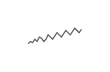
\begin{tikzpicture}[x=0.08em, y=0.08em, line width=0.4pt]
                \draw[FooterGray] (0,3) -- (1,4) -- (2,3.5) -- (3,5) -- (4,4) -- (5,6) -- (6,5.5) -- (7,4) -- (8,5) -- (9,7) -- (10,6) -- (11,5) -- (12,6.5) -- (13,8) -- (14,7) -- (15,6) -- (16,7.5) -- (17,9) -- (18,8) -- (19,7) -- (20,8.5) -- (21,10) -- (22,9) -- (23,8) -- (24,9.5);
            \end{tikzpicture}%
        }%
        \hskip0.5cm%
    }%
    \vskip6pt%
}

%=============================================================================
% PACKAGES
%=============================================================================
\usepackage[utf8]{inputenc}
\DeclareUnicodeCharacter{03B1}{\ensuremath{\alpha}}
\usepackage[T1]{fontenc}
\usepackage{amsmath, amssymb, amsthm}
\usepackage{mathtools}
\usepackage{bm}
\usepackage{tikz}
\usetikzlibrary{arrows.meta, positioning, shapes, calc, decorations.pathreplacing, shadings}
\usepackage{booktabs}
\usepackage{multirow}
\usepackage{array}
\usepackage{graphicx}
\usepackage{animate}
\usepackage{hyperref}
\usepackage{colortbl}
\usepackage{listings}
\lstset{language=Python, basicstyle=\ttfamily\scriptsize, keywordstyle=\color{MainBlue}\bfseries,
  commentstyle=\color{Forest}, stringstyle=\color{Crimson}, breaklines=true,
  frame=none, backgroundcolor=\color{VeryLightGray}, xleftmargin=2mm}
\hypersetup{colorlinks=true, linkcolor=MainBlue, urlcolor=MainBlue}
\graphicspath{{../../logos/}{../../charts/}{../../photos/}}
\usepackage{xcolor}
\hfuzz=2pt  % Suppress tiny overfull warnings (<2pt)
\vfuzz=2pt  % Suppress tiny vertical overfull warnings (<2pt)
% \mathrm in the sans-serif family of the slides (beamer resets \mathrm to the serif family at \begin{document};
% this hook runs after beamer's, so WN, Var, RMSE, ... in formulas match the surrounding text)
% Bold vectors and matrices in the same sans-serif family: \mathbf{A} in sans bold (beamer's own \mathbf came out in
% medium weight), and the bold upright Greek capitals of \boldsymbol / \bm (\bSigma, \bPhi, \boldsymbol{\Theta}) in
% cmss bold: bm.sty fixes its "boldoperators" font when it is loaded (serif cmbx), before beamer switches the
% operators to cmss, so it is reset here.
\AtBeginDocument{%
  \SetMathAlphabet{\mathrm}{normal}{\encodingdefault}{\sfdefault}{\mddefault}{n}%
  \SetMathAlphabet{\mathrm}{bold}{\encodingdefault}{\sfdefault}{bx}{n}%
  \SetMathAlphabet{\mathbf}{normal}{\encodingdefault}{\sfdefault}{bx}{n}%
  \SetMathAlphabet{\mathbf}{bold}{\encodingdefault}{\sfdefault}{bx}{n}%
  \SetSymbolFont{boldoperators}{normal}{OT1}{cmss}{bx}{n}%
  \SetSymbolFont{boldoperators}{bold}{OT1}{cmss}{bx}{n}}

%=============================================================================
% QUANTLET COMMANDS
%   \quantlet{<displayed name>}{<url>}       (generic, compatible with the older TSA decks)
%   \tsaquantlet{Ch_05}{TSA_ch5_garch}       -> https://github.com/danpele/Time-Series-Analysis/tree/main/Quantlets/Ch_05/TSA_ch5_garch
%   \qlurl{<folder>} is defined per chapter by the generator (Quantlets/Ch_NN/<folder>)
%=============================================================================
\newcommand{\tsarepo}{https://github.com/danpele/Time-Series-Analysis}
\newcommand{\tsaqlbase}{https://github.com/danpele/Time-Series-Analysis/tree/main/Quantlets}
\newcommand{\quantlet}[2]{%
    \hfill\href{#2}{%
        \raisebox{-0.15em}{
\includegraphics[height=0.7em]{ql_logo.png}}%
        \textcolor{MainBlue}{\tiny\ #1}%
    }%
}
\newcommand{\tsaquantlet}[2]{\quantlet{\detokenize{#2}}{\tsaqlbase/#1/#2}}

%=============================================================================
% NOTEBOOKS (Google Colab)
%   \colaburl{notebooks/EN/chapter5_seminar_notebook.ipynb} -> the Colab link of a file in the TSA repo
%   \nb: the chapter notebook (each seminar deck redefines it with \renewcommand)
%=============================================================================
\newcommand{\colaburl}[1]{https://colab.research.google.com/github/danpele/Time-Series-Analysis/blob/main/#1}
\newcommand{\nb}{https://colab.research.google.com/github/danpele/Time-Series-Analysis/tree/main/notebooks/EN}
\newcommand{\nbname}{notebooks/EN}

%=============================================================================
% SLIDE HELPERS (used by the generators; the same as in MFM)
%=============================================================================
% local font size for list bodies (the preamble forces \normalsize)
\newcommand{\itemsize}[1]{\setbeamertemplate{itemize/enumerate body begin}{#1}\setbeamertemplate{itemize/enumerate subbody begin}{#1}}
\newcommand{\intitle}[1]{{\hypersetup{urlcolor=white}#1}}   % white links inside coloured title bars
\newcommand{\imgcap}[1]{{\scriptsize #1}\\[0.5mm]}          % caption under a photo
\newcommand{\imgcredit}[2]{{\tiny\color{FooterGray}\href{#1}{#2}}}   % image credit: source URL, author/licence
\newcommand{\aiprompt}[1]{{\ttfamily\color{MainBlue}#1}}     % a prompt to an AI assistant

%=============================================================================
% SEMINARS: student version by default; the instructor wrapper *_solutions.tex sets \solutionstrue
%=============================================================================
\makeatletter\@ifundefined{ifsolutions}{\expandafter\newif\csname ifsolutions\endcsname}{}\makeatother
\newcommand{\solonly}[1]{\ifsolutions #1\fi}
\newcommand{\propsub}{\ifsolutions\else\framesubtitle{\ifdefined\tsalang Rezolvarea se discută la seminar\else Solution discussed in class\fi}\fi}

%=============================================================================
% APPENDIX AND CHAPTER LINKS (latex/appendix_links.py writes the calls; it also re-declares these
% macros before \begin{document}, so the decks compile with or without this preamble block)
%=============================================================================
\providecommand{\tsaapplink}[3]{\hypertarget{#2}{}\hyperlink{#1}{\beamergotobutton{#3}}}
\providecommand{\tsaappback}[2]{\begin{tikzpicture}[remember picture,overlay]\node[anchor=south east] at ([xshift=-3mm,yshift=7mm]current page.south east){\hyperlink{#1}{\beamerreturnbutton{#2}}};\end{tikzpicture}}
\providecommand{\tsachlink}[2]{\href{#1}{#2}}
\providecommand{\tsachlinkt}[2]{\href{#1}{\usebeamercolor[fg]{frametitle}#2}}

%=============================================================================
% QUANTINAR COMMAND: link către un curs Quantinar (subiecte avansate)
%=============================================================================
\newcommand{\quantinar}[2]{%
    \href{#2}{%
        \raisebox{-0.15em}{
\includegraphics[height=0.8em]{qr_logo.png}}%
        \textcolor{MainBlue}{\scriptsize\ #1}%
    }%
}

%=============================================================================
% CUSTOM TITLE PAGE
%=============================================================================
\defbeamertemplate*{title page}{hybrid}[1][]
{
    \vspace{0.2cm}
    % Logos row - top header (with clickable links)
    \begin{center}
        \href{https://www.ase.ro}{
\includegraphics[height=1.0cm]{ase_logo.png}}\hspace{0.3cm}%
        \href{https://theida.net}{
\includegraphics[height=1.0cm]{ida_logo.png}}\hspace{0.3cm}%
        \href{https://blockchain-research-center.com}{
\includegraphics[height=1.0cm]{brc_logo.png}}\hspace{0.3cm}%
        \href{https://www.ai4efin.ase.ro}{
\includegraphics[height=1.0cm]{ai4efin_logo.png}}\hspace{0.3cm}%
        \href{https://ipe.ro/new}{
\includegraphics[height=1.0cm]{acad_logo.png}}\hspace{0.3cm}%
        \href{https://www.digital-finance-msca.com}{
\includegraphics[height=1.0cm]{msca_logo.png}}%
    \end{center}

    \vspace{0.6cm}

    % Main title with Q logos on sides (with clickable links)
    \begin{center}
        \begin{minipage}{0.1\textwidth}
            \centering
            \href{https://quantlet.com}{
\includegraphics[height=1.1cm]{ql_logo.png}}
        \end{minipage}%
        \begin{minipage}{0.78\textwidth}
            \centering
            {\LARGE\bfseries\usebeamercolor[fg]{title}\inserttitle}

            \vspace{0.3cm}

            {\usebeamerfont{subtitle}\usebeamercolor[fg]{title}\insertsubtitle}
        \end{minipage}%
        \begin{minipage}{0.1\textwidth}
            \centering
            \href{https://quantinar.com}{
\includegraphics[height=1.1cm]{qr_logo.png}}
        \end{minipage}
    \end{center}

    \vspace{0.6cm}

    % Authors (left aligned)
    \hspace{0.5cm}{\usebeamerfont{author}\insertauthor}

    \vspace{0.3cm}

    % Institute/Affiliations (left aligned)
    \hspace{0.5cm}\begin{minipage}[t]{0.9\textwidth}
        \raggedright\small\insertinstitute
    \end{minipage}
}

%=============================================================================
% THEOREM ENVIRONMENTS
%=============================================================================
\theoremstyle{definition}
\setbeamertemplate{theorems}[numbered]
\ifdefined\tsalang
\newtheorem{defn}{Definiție}
\newtheorem{thm}{Teoremă}
\newtheorem{prop}{Propoziție}
\newtheorem{rmk}{Observație}
\else
\newtheorem{defn}{Definition}
\newtheorem{thm}{Theorem}
\newtheorem{prop}{Proposition}
\newtheorem{rmk}{Remark}
\fi

%=============================================================================
% CENTRED MINIPAGE (no extra vertical space)
%=============================================================================
\newenvironment{cminipage}[1]{%
    \par\noindent\hfill\begin{minipage}{#1}\ignorespaces
}{%
    \end{minipage}\hfill\null\par
}

%=============================================================================
% CUSTOM COMMANDS
%=============================================================================
\newcommand{\E}{\mathbb{E}}
\newcommand{\Var}{\text{Var}}
\newcommand{\Cov}{\text{Cov}}
\newcommand{\Corr}{\text{Corr}}
\newcommand{\R}{\mathbb{R}}
\newcommand{\N}{\mathbb{N}}
\newcommand{\Z}{\mathbb{Z}}
\newcommand{\B}{\mathbf{B}}
\newcommand{\imark}{\textcolor{MainBlue}{\textbullet}}
\newcommand{\RMSE}{\text{RMSE}}
\newcommand{\MAE}{\text{MAE}}
\newcommand{\MAPE}{\text{MAPE}}

% Boldface vector/matrix commands (VAR, VECM, state space; also used by the older TSA decks)
\newcommand{\bY}{\mathbf{Y}}
\newcommand{\bX}{\mathbf{X}}
\newcommand{\bA}{\mathbf{A}}
\newcommand{\bB}{\mathbf{B}}
\newcommand{\bepsilon}{\boldsymbol{\varepsilon}}
\newcommand{\bSigma}{\boldsymbol{\Sigma}}
\newcommand{\bPhi}{\boldsymbol{\Phi}}
\newcommand{\bGamma}{\boldsymbol{\Gamma}}
\newcommand{\bPi}{\boldsymbol{\Pi}}
\newcommand{\bc}{\mathbf{c}}
\newcommand{\balpha}{\boldsymbol{\alpha}}
\newcommand{\bbeta}{\boldsymbol{\beta}}
\newcommand{\bvarepsilon}{\boldsymbol{\varepsilon}}

% Legacy seminar marks (older TSA seminar decks)
\newcommand{\correct}{\textcolor{Forest}{\checkmark}}
\newcommand{\incorrect}{\textcolor{Crimson}{\texttimes}}


\newcommand{\qlurl}[1]{https://github.com/danpele/Time-Series-Analysis/tree/main/Quantlets/Ch_03/#1}

% Clickable citations (DOIs verified via Crossref)
\newcommand{\refHP}{\href{https://doi.org/10.1007/978-3-031-13584-2}{Huang și Petukhina (2022)}}
\newcommand{\refFPP}{\href{https://otexts.com/fpp3/}{Hyndman și Athanasopoulos (2021)}}
\newcommand{\refBD}{\href{https://doi.org/10.1007/978-3-319-29854-2}{Brockwell și Davis (2016)}}
\newcommand{\refHamilton}{\href{https://doi.org/10.2307/j.ctv14jx6sm}{Hamilton (1994)}}
\newcommand{\refBJ}{\href{https://doi.org/10.1002/9781118619193}{Box, Jenkins și Reinsel (2008)}}
\newcommand{\refDF}{\href{https://doi.org/10.1080/01621459.1979.10482531}{Dickey și Fuller (1979)}}
\newcommand{\refDFb}{\href{https://doi.org/10.2307/1912517}{Dickey și Fuller (1981)}}
\newcommand{\refFuller}{\href{https://doi.org/10.1002/9780470316917}{Fuller (1996)}}
\newcommand{\refSD}{\href{https://doi.org/10.1093/biomet/71.3.599}{Said și Dickey (1984)}}
\newcommand{\refPP}{\href{https://doi.org/10.1093/biomet/75.2.335}{Phillips și Perron (1988)}}
\newcommand{\refKPSS}{\href{https://doi.org/10.1016/0304-4076(92)90104-Y}{Kwiatkowski et al.\ (1992)}}
\newcommand{\refMacKinnon}{\href{https://doi.org/10.1080/07350015.1994.10510005}{MacKinnon (1994)}}
\newcommand{\refMacKinnonb}{\href{https://ideas.repec.org/p/qed/wpaper/1227.html}{MacKinnon (2010)}}
\newcommand{\refGN}{\href{https://doi.org/10.1016/0304-4076(74)90034-7}{Granger și Newbold (1974)}}
\newcommand{\refPhillips}{\href{https://doi.org/10.1016/0304-4076(86)90001-1}{Phillips (1986)}}
\newcommand{\refYule}{\href{https://doi.org/10.2307/2341482}{Yule (1926)}}
\newcommand{\refNP}{\href{https://doi.org/10.1016/0304-3932(82)90012-5}{Nelson și Plosser (1982)}}
\newcommand{\refNK}{\href{https://doi.org/10.2307/1911520}{Nelson și Kang (1981)}}
\newcommand{\refPerron}{\href{https://doi.org/10.2307/1913712}{Perron (1989)}}
\newcommand{\refZA}{\href{https://doi.org/10.1080/07350015.1992.10509904}{Zivot și Andrews (1992)}}
\newcommand{\refBaiP}{\href{https://doi.org/10.2307/2998540}{Bai și Perron (1998)}}
\newcommand{\refSchwert}{\href{https://doi.org/10.1080/07350015.1989.10509723}{Schwert (1989)}}
\newcommand{\refNgP}{\href{https://doi.org/10.1111/1468-0262.00256}{Ng și Perron (2001)}}
\newcommand{\refERS}{\href{https://doi.org/10.2307/2171846}{Elliott, Rothenberg și Stock (1996)}}
\newcommand{\refDP}{\href{https://doi.org/10.1080/07350015.1987.10509614}{Dickey și Pantula (1987)}}
\newcommand{\refPS}{\href{https://doi.org/10.1016/0304-4076(77)90015-x}{Plosser și Schwert (1977)}}
\newcommand{\refHK}{\href{https://doi.org/10.18637/jss.v027.i03}{Hyndman și Khandakar (2008)}}
\newcommand{\refMR}{\href{https://doi.org/10.1016/0022-1996(83)90017-X}{Meese și Rogoff (1983)}}
\newcommand{\refEG}{\href{https://doi.org/10.2307/1913236}{Engle și Granger (1987)}}
\newcommand{\refLB}{\href{https://doi.org/10.1093/biomet/65.2.297}{Ljung și Box (1978)}}

\title[Serii de timp]{Serii de timp}
\subtitle{Capitolul 3: Rădăcini unitare și modele ARIMA}
\author[D.T. Pele]{Daniel Traian PELE}
\institute{Academia de Studii Economice din București\\
IDA Institute Digital Assets\\
Blockchain Research Center\\
AI4EFin Artificial Intelligence for Energy Finance\\
Academia Română, Institutul de Prognoză Economică\\
MSCA Digital Finance}
\date{}

%=============================================================================
\providecommand{\tsaapplink}[3]{\hypertarget{#2}{}\hyperlink{#1}{\beamergotobutton{#3}}}  % APPLINKS-MACROS
\providecommand{\tsaappback}[2]{\begin{tikzpicture}[remember picture,overlay]\node[anchor=south east] at ([xshift=-3mm,yshift=7mm]current page.south east){\hyperlink{#1}{\beamerreturnbutton{#2}}};\end{tikzpicture}}  % APPLINKS-MACROS
\providecommand{\tsachlink}[2]{\href{#1}{#2}}  % APPLINKS-MACROS
\providecommand{\tsachlinkt}[2]{\href{#1}{\usebeamercolor[fg]{frametitle}#2}}  % APPLINKS-MACROS
\begin{document}
%=============================================================================

{
\setbeamertemplate{headline}{}
\setbeamertemplate{footline}{}
\begin{frame}[noframenumbering]
    \titlepage
\end{frame}
}
% BEGIN-ACRONYMS (generat de latex/acronyms.py; nu editati manual)
\begin{frame}{Acronime folosite în acest material (1/2)}
\setbeamertemplate{itemize/enumerate body begin}{\footnotesize}
\begin{columns}[T]
\begin{column}{0.49\textwidth}
\begin{itemize}\setlength{\itemsep}{0pt}
    \item \textbf{ACF}: Autocorrelation Function (funcția de autocorelație)
    \item \textbf{ADF}: Augmented Dickey–Fuller (test) — testul Dickey–Fuller augmentat
    \item \textbf{AI}: Artificial Intelligence (inteligență artificială)
    \item \textbf{AIC}: Akaike Information Criterion (criteriul informațional Akaike)
    \item \textbf{AR}: AutoRegressive (model) — model autoregresiv
    \item \textbf{ARIMA}: AutoRegressive Integrated Moving Average (model) — model autoregresiv integrat cu medie mobilă
    \item \textbf{ARMA}: AutoRegressive Moving Average (model) — model autoregresiv cu medie mobilă
    \item \textbf{BET}: Bucharest Exchange Trading (index) — indicele de referință al Bursei de Valori București
    \item \textbf{BIC}: Bayesian Information Criterion (criteriul informațional bayesian al lui Schwarz)
\end{itemize}
\end{column}
\begin{column}{0.49\textwidth}
\begin{itemize}\setlength{\itemsep}{0pt}
    \item \textbf{BNR}: Banca Națională a României
    \item \textbf{CUSUM}: CUmulative SUM (control chart) — graficul sumelor cumulate
    \item \textbf{DF}: Dickey–Fuller (test) — testul Dickey–Fuller
    \item \textbf{DF-GLS}: Dickey–Fuller test with GLS detrending (testul Dickey–Fuller cu eliminarea trendului prin GLS)
    \item \textbf{DW}: Durbin–Watson (statistic) — statistica Durbin–Watson
    \item \textbf{FRED}: Federal Reserve Economic Data (baza de date economice a Rezervei Federale din St. Louis)
    \item \textbf{GDP}: Gross Domestic Product (produsul intern brut)
    \item \textbf{GLS}: Generalised Least Squares (metoda generalizată a celor mai mici pătrate)
    \item \textbf{IAPC}: Indicele armonizat al prețurilor de consum
\end{itemize}
\end{column}
\end{columns}
\end{frame}
\begin{frame}{Acronime folosite în acest material (2/2)}
\setbeamertemplate{itemize/enumerate body begin}{\footnotesize}
\begin{columns}[T]
\begin{column}{0.49\textwidth}
\begin{itemize}\setlength{\itemsep}{0pt}
    \item \textbf{KPSS}: Kwiatkowski–Phillips–Schmidt–Shin (test) — testul de staționaritate Kwiatkowski–Phillips–Schmidt–Shin
    \item \textbf{MA}: Moving Average (medie mobilă)
    \item \textbf{MAIC}: Modified Akaike Information Criterion (criteriul informațional Akaike modificat)
    \item \textbf{OLS}: Ordinary Least Squares (metoda celor mai mici pătrate)
    \item \textbf{PACF}: Partial AutoCorrelation Function (funcția de autocorelație parțială)
    \item \textbf{PIB}: Produsul intern brut
    \item \textbf{PNB}: Produsul național brut
    \item \textbf{PP}: Phillips–Perron (test) — testul Phillips–Perron de rădăcină unitară
\end{itemize}
\end{column}
\begin{column}{0.49\textwidth}
\begin{itemize}\setlength{\itemsep}{0pt}
    \item \textbf{RMSE}: Root Mean Squared Error (rădăcina erorii pătratice medii)
    \item \textbf{SARIMA}: Seasonal ARIMA (model) — model ARIMA sezonier
    \item \textbf{SE}: Standard Error (eroare standard)
    \item \textbf{SUA}: Statele Unite ale Americii
    \item \textbf{TBATS}: Trigonometric seasonality, Box–Cox, ARMA errors, Trend, Seasonal components (model) — model cu sezonalitate trigonometrică, transformare Box–Cox, erori ARMA, trend și componente sezoniere
    \item \textbf{UE}: Uniunea Europeană
    \item \textbf{VAR}: Vector AutoRegression (model vector autoregresiv)
    \item \textbf{ZA}: Zivot–Andrews (test) — testul Zivot–Andrews cu o ruptură structurală
\end{itemize}
\end{column}
\end{columns}
\end{frame}
% END-ACRONYMS

\begin{frame}{Întrebarea de azi și traseul}
\itemsize{\small}
\begin{itemize}
    \item \textbf{Întrebarea}: cînd o serie urcă în timp, este șocul de azi temporar sau permanent și cum trebuie prognozată seria?
    \begin{itemize}
        \item răspunsul decide dacă eliminăm trendul sau diferențiem seria și cît de largi sînt intervalele de prognoză
    \end{itemize}
    \item \textbf{Traseul} capitolului
    \begin{itemize}
        \item trend determinist și trend stochastic; procese integrate $I(d)$; regresia falsă
        \item teste de rădăcină unitară: Dickey--Fuller, ADF, Phillips--Perron; testul de staționaritate KPSS; rupturi structurale
        \item modele ARIMA$(p,d,q)$: identificare, estimare, diagnosticare, prognoze cu intervale tot mai largi
    \end{itemize}
    \item Pornim de la \tsachlink{https://danpele.github.io/Time-Series-Analysis/RO/Cursuri/capitol1_procese_stochastice_stationaritate.pdf}{Capitolul 1} (staționaritate, mers aleator, diferențiere) și de la \tsachlink{https://danpele.github.io/Time-Series-Analysis/RO/Cursuri/capitol2_modele_arma.pdf}{Capitolul 2} (modele ARMA); Seminarul 3 are loc înaintea acestui curs
\end{itemize}
\end{frame}

\begin{frame}{Rezultatele învățării}
\itemsize{\small}
\begin{itemize}
    \item Deosebiți seriile staționare în jurul trendului de cele staționare în diferențe și explicați de ce contează deosebirea
    \item Recunoașteți o regresie falsă și explicați de ce apare
    \item Aplicați și interpretați testele ADF, Phillips--Perron și KPSS, cu termenii determiniști și numărul de laguri potrivite
    \item Explicați cum poate o ruptură structurală să imite o rădăcină unitară
    \item Identificați, estimați, verificați și folosiți pentru prognoză un model ARIMA$(p,d,q)$ și explicați de ce intervalele lui cresc cu orizontul
    \item Folosiți critic selecția automată a modelelor ARIMA
\end{itemize}
\end{frame}

\begin{frame}{Bibliografie și instrumente}
\itemsize{\small}
\begin{itemize}
    \item Manual: \refHP, cap.~4--5 (modele ARIMA și nestaționaritate)
    \begin{itemize}
        \item manual însoțitor, gratuit online: \refFPP, cap.~9 (modele ARIMA)
    \end{itemize}
    \item Teorie: \refHamilton, cap.~15--17 (trenduri, rădăcini unitare); \refBJ\ pentru metodologia ARIMA
    \item Quantlet-urile Python ale capitolului: \href{https://github.com/danpele/Time-Series-Analysis/tree/main/Quantlets/Ch_03}{Quantlets/Ch\_03}
    \begin{itemize}
        \item \texttt{adfuller}, \texttt{kpss}, \texttt{zivot\_andrews} și \texttt{ARIMA} din \texttt{statsmodels}; testul Phillips--Perron scris în cîteva rînduri
    \end{itemize}
    \item Notebook-ul cursului: \href{\colaburl{notebooks/EN/chapter3_lecture_notebook.ipynb}}{deschideți în Google Colab}
    \item Curs video: \quantinar{Applied Time Series Analysis with Python}{https://quantinar.com/course/137/applied-time-series-analysis-with-python}
\end{itemize}
\end{frame}


%=============================================================================
\section{Trend determinist și trend stochastic}
%=============================================================================

\begin{frame}{Patru serii care urcă în timp}
\itemsize{\footnotesize}
\begin{center}
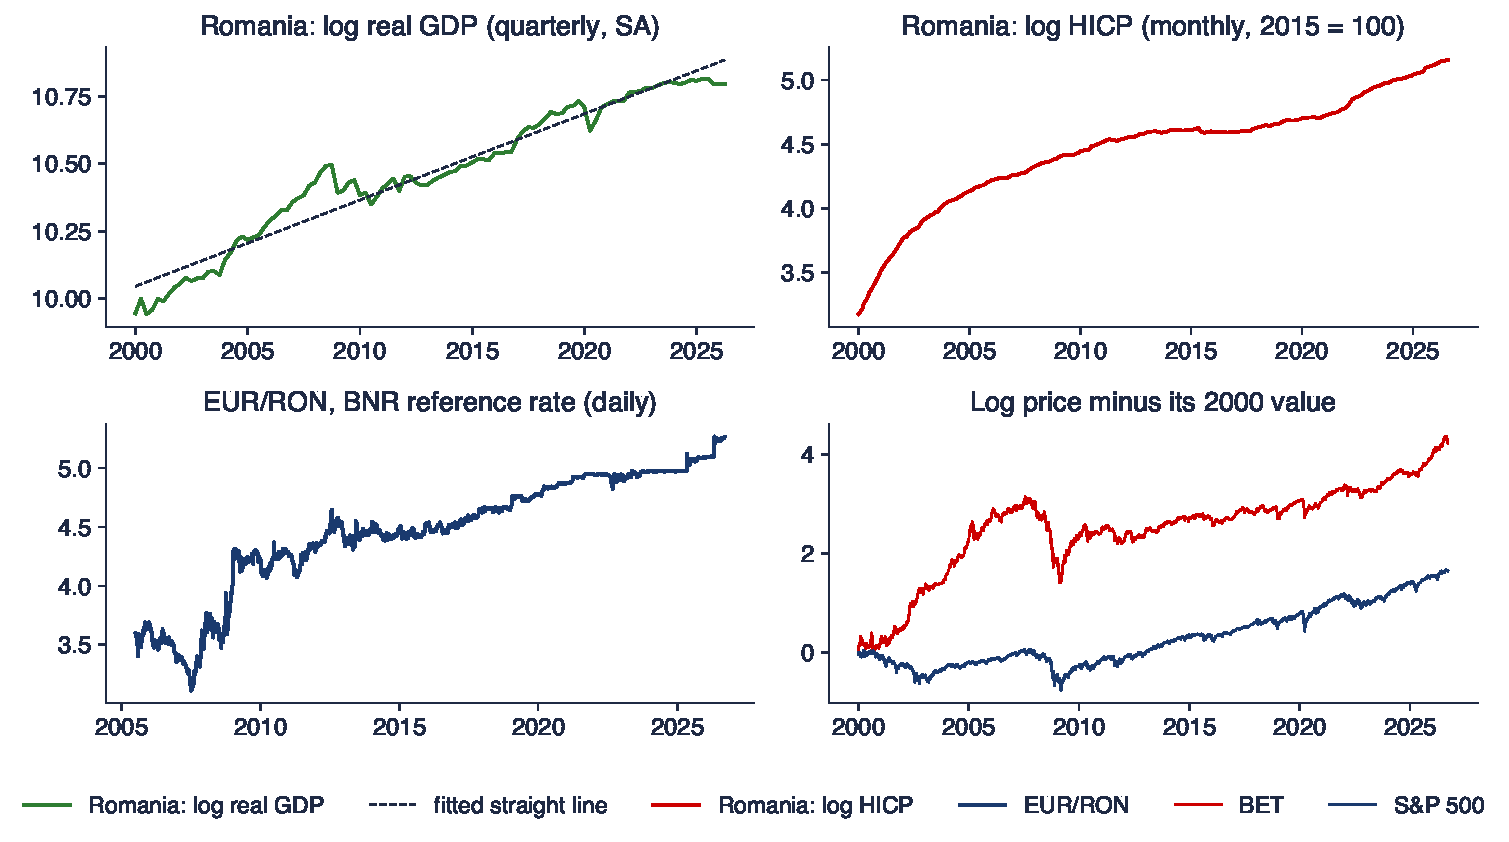
\includegraphics[width=0.97\textwidth,height=0.66\textheight,keepaspectratio]{tsa_ch3_four_series.pdf}
\end{center}
\vspace{-0.25cm}
\begin{itemize}
    \item PIB-ul real (Eurostat, ajustat sezonier) și IAPC ale României (Eurostat); cursul EUR/RON, cursul de referință BNR; logaritmii prețurilor BET și S\&P 500, zilnic din 2000
    \item Niciuna nu are o medie constantă: în \tsachlink{https://danpele.github.io/Time-Series-Analysis/RO/Cursuri/capitol1_procese_stochastice_stationaritate.pdf}{Capitolul 1} le-am numit nestaționare
\end{itemize}
\quantlet{TSA\_ch3\_trends}{\qlurl{TSA_ch3_trends}}
\end{frame}

\begin{frame}{Interpretarea celor patru serii}
\itemsize{\small}
\begin{itemize}
    \item PIB-ul crește în medie cu 0{,}80\% pe trimestru (circa 3{,}2\% pe an), dar se abate de la dreaptă cu pînă la 18\%
    \begin{itemize}
        \item recesiunea din 2009: a revenit PIB-ul la vechea dreaptă sau a pornit pe una nouă?
    \end{itemize}
    \item Prețurile de consum: $\times$7{,}2 din 2000; EUR/RON: de la 3{,}60 la 5{,}26 lei; BET: $+426$ puncte logaritmice, S\&P 500: $+166$ puncte logaritmice (pînă la 18 septembrie 2026)
    \item Două modele pot produce asemenea grafice
    \begin{itemize}
        \item o dreaptă fixă plus zgomot staționar (\textbf{trend determinist})
        \item un mers aleator cu derivă (\textbf{trend stochastic})
    \end{itemize}
\end{itemize}
\end{frame}

\begin{frame}{Serii staționare în jurul trendului}
\itemsize{\small}
\begin{itemize}
    \item \textbf{Definiție}: $y_t = \alpha + \beta t + u_t$, unde $u_t$ este un proces staționar (de exemplu un AR(1) staționar, \tsachlink{https://danpele.github.io/Time-Series-Analysis/RO/Cursuri/capitol2_modele_arma.pdf}{Capitolul 2})
    \begin{itemize}
        \item $\alpha$: termenul liber; $\beta$: panta, adică variația medie pe perioadă; $t$: indicele de timp
        \item $y_t$ este \textbf{staționar în jurul trendului}: staționar după ce scădem dreapta $\alpha + \beta t$
    \end{itemize}
    \item Proprietăți
    \begin{itemize}
        \item $E[y_t] = \alpha + \beta t$; $\mathrm{Var}(y_t) = \mathrm{Var}(u_t)$, constantă
        \item un șoc îndepărtează $y_t$ de dreaptă doar temporar: cu $u_t = \phi u_{t-1} + \varepsilon_t$, efectul lui după $h$ perioade este $\phi^h$
        \item prognozele pe termen lung revin la dreaptă; intervalele lor au o lățime mărginită
    \end{itemize}
    \item Tratamentul corect: estimăm trendul prin OLS (ordinary least squares, metoda celor mai mici pătrate) și modelăm reziduurile ca ARMA
\end{itemize}
\end{frame}

\begin{frame}{Serii staționare în diferențe}
\itemsize{\small}
\begin{itemize}
    \item \textbf{Definiție}: $y_t = \beta + y_{t-1} + u_t$, $u_t$ staționar; prin substituție, $y_t = y_0 + \beta t + \sum_{i=1}^{t} u_i$
    \begin{itemize}
        \item $\beta$: deriva, adică variația medie pe perioadă; $y_0$: valoarea inițială
        \item $y_t$ este \textbf{staționar în diferențe}: $\Delta y_t = \beta + u_t$ este staționar
        \item $\sum_{i \le t} u_i$ este \textbf{trendul stochastic}; $\beta t$ provine din derivă
    \end{itemize}
    \item Proprietăți
    \begin{itemize}
        \item aceeași medie $y_0 + \beta t$ ca la o serie staționară în jurul trendului, dar $\mathrm{Var}(y_t)$ crește cu $t$ (\tsachlink{https://danpele.github.io/Time-Series-Analysis/RO/Cursuri/capitol1_procese_stochastice_stationaritate.pdf}{Capitolul 1}: $t\sigma^2$ pentru un mers aleator)
        \item fiecare șoc rămîne pentru totdeauna în nivel: nu există o dreaptă la care seria să revină
        \item intervalele de prognoză se lărgesc fără limită pe măsură ce orizontul crește
    \end{itemize}
    \item Tratamentul corect: diferențiem seria și modelăm $\Delta y_t$ ca ARMA: modelul ARIMA din acest capitol
\end{itemize}
\end{frame}

\begin{frame}{Aceeași derivă, memorie diferită}
\itemsize{\footnotesize}
\begin{center}
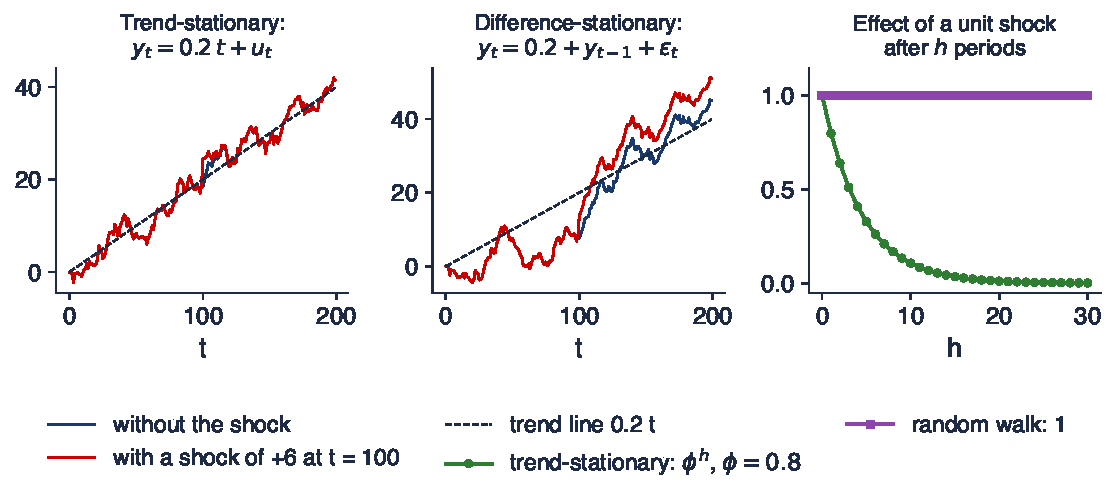
\includegraphics[width=0.97\textwidth,height=0.54\textheight,keepaspectratio]{tsa_ch3_ts_ds.pdf}
\end{center}
\vspace{-0.25cm}
\begin{itemize}
    \item Stînga și centru: aceleași șocuri generează o serie staționară în jurul trendului ($u_t$ AR(1), $\phi = 0{,}8$) și un mers aleator cu deriva 0,2; traiectoriile roșii adaugă un șoc de $+6$ la $t = 100$
    \item Dreapta: efectul unui șoc unitar după $h$ perioade
\end{itemize}
\quantlet{TSA\_ch3\_trends}{\qlurl{TSA_ch3_trends}}
\end{frame}

\begin{frame}{Interpretarea celor două trenduri}
\itemsize{\small}
\begin{itemize}
    \item Seria staționară în jurul trendului: șocul se stinge; efectul lui este $0{,}8^{10} = 0{,}107$ după 10 perioade și $0{,}012$ după 20
    \begin{itemize}
        \item la $t = 200$ traiectoriile roșie și albastră coincid
    \end{itemize}
    \item Mersul aleator: întreaga traiectorie urcă cu 6 și rămîne acolo
    \begin{itemize}
        \item o recesiune într-o economie de tip staționar în diferențe este o pierdere permanentă de producție, nu o scădere temporară sub trend
    \end{itemize}
    \item Cu ochiul liber, cele două serii fără șoc arată la fel: avem nevoie de un test formal (secțiunile 3--4)
\end{itemize}
\end{frame}

\begin{frame}{Procese integrate}
\itemsize{\small}
\begin{itemize}
    \item \textbf{Definiție}: $y_t$ este \textbf{integrat de ordinul $d$}, $y_t \sim I(d)$, dacă $\Delta^d y_t$ este staționar, iar $\Delta^{d-1}y_t$ nu este
    \begin{itemize}
        \item $I(0)$: staționar (cu o reprezentare ARMA inversabilă, \tsachlink{https://danpele.github.io/Time-Series-Analysis/RO/Cursuri/capitol2_modele_arma.pdf}{Capitolul 2}); $I(1)$: staționar după o diferențiere; $I(2)$: după două
        \item $\Delta^2 y_t = \Delta y_t - \Delta y_{t-1} = y_t - 2y_{t-1} + y_{t-2}$
    \end{itemize}
    \item Ordine tipice în economie și finanțe
    \begin{itemize}
        \item logaritmii prețurilor acțiunilor, cursurile de schimb, logaritmul PIB: $I(1)$; randamentele și ratele de creștere: $I(0)$
        \item nivelul prețurilor în perioade cu inflație ridicată: posibil $I(2)$, deci inflația însăși ar fi $I(1)$
    \end{itemize}
    \item Reguli
    \begin{itemize}
        \item $I(0) + I(1) = I(1)$: trendul stochastic domină; o serie staționară în jurul trendului este $I(0)$ după eliminarea trendului, nu după diferențiere
    \end{itemize}
\end{itemize}
\end{frame}

\begin{frame}{Rădăcina unitară}
\itemsize{\small}
\begin{itemize}
    \item Scriem un AR($p$) cu operatorul lag $L$ (\tsachlink{https://danpele.github.io/Time-Series-Analysis/RO/Cursuri/capitol1_procese_stochastice_stationaritate.pdf}{Capitolul 1}): $\phi(L)y_t = \varepsilon_t$, $\phi(z) = 1 - \phi_1 z - \dots - \phi_p z^p$
    \begin{itemize}
        \item \tsachlink{https://danpele.github.io/Time-Series-Analysis/RO/Cursuri/capitol2_modele_arma.pdf}{Capitolul 2}: staționar dacă toate rădăcinile ecuației $\phi(z) = 0$ sînt în afara cercului unitate, $|z| > 1$
    \end{itemize}
    \item \textbf{Rădăcină unitară}: o rădăcină este $z = 1$, deci $\phi(z) = (1 - z)\,\phi^*(z)$, iar rădăcinile lui $\phi^*$ sînt în afara cercului
    \begin{itemize}
        \item atunci $\phi^*(L)\,\Delta y_t = \varepsilon_t$: $\Delta y_t$ este un AR($p-1$) staționar, iar $y_t \sim I(1)$
        \item AR(1): $\phi(z) = 1 - \phi z$ are rădăcina $1/\phi$, unitară cînd $\phi = 1$: mersul aleator
    \end{itemize}
    \item \textbf{Exemplu}: $y_t = 1{,}5y_{t-1} - 0{,}5y_{t-2} + \varepsilon_t$; $1 - 1{,}5z + 0{,}5z^2 = (1 - z)(1 - 0{,}5z)$
    \begin{itemize}
        \item rădăcinile 1 și 2: $\Delta y_t = 0{,}5\,\Delta y_{t-1} + \varepsilon_t$, un AR(1) în diferențe
    \end{itemize}
\end{itemize}
\end{frame}

\begin{frame}{Studiu de caz: Nelson și Plosser (1982)}
\itemsize{\small}
\begin{itemize}
    \item \textbf{Întrebarea}: sînt seriile macroeconomice ale SUA staționare în jurul unui trend, cum presupuneau modelele ciclului economic din anii 1970?
    \begin{itemize}
        \item \refNP: 14 serii anuale lungi (PNB real, ocuparea, prețurile, salariile, ratele dobînzii, prețurile acțiunilor), unele din 1860
    \end{itemize}
    \item \textbf{Metoda}: testul Dickey--Fuller din secțiunea 3, cu constantă și trend
    \begin{itemize}
        \item rădăcina unitară a fost respinsă pentru o singură serie, rata șomajului
    \end{itemize}
    \item \textbf{Consecința}: șocurile asupra producției par permanente, nu temporare
    \begin{itemize}
        \item o dezbatere amplă despre natura recesiunilor și un avertisment împotriva eliminării trendului printr-o dreaptă (slide-ul următor)
        \item concluzia a fost contestată ulterior prin rupturi structurale (secțiunea 5)
    \end{itemize}
\end{itemize}
\end{frame}

\begin{frame}{Eliminarea trendului dintr-un mers aleator}
\itemsize{\footnotesize}
\begin{center}
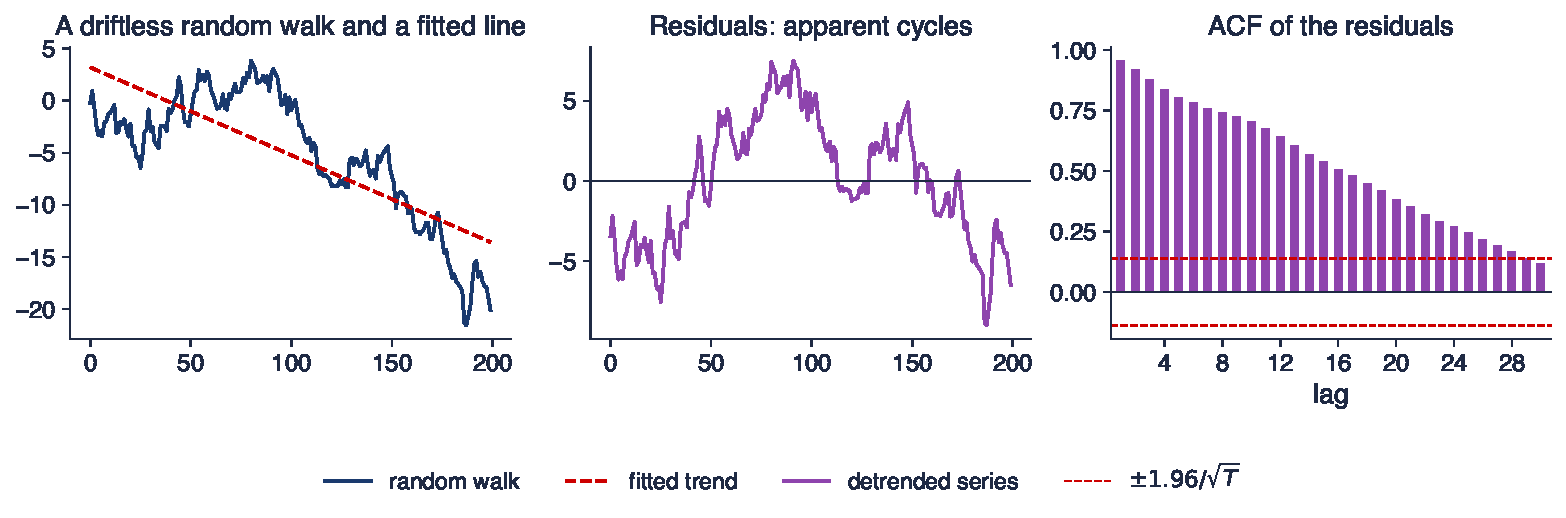
\includegraphics[width=0.97\textwidth,height=0.56\textheight,keepaspectratio]{tsa_ch3_detrend.pdf}
\end{center}
\vspace{-0.25cm}
\begin{itemize}
    \item Stînga: un mers aleator fără derivă ($T = 200$) și dreapta OLS $\hat a + \hat b t$; centru: reziduurile; dreapta: ACF a reziduurilor
\end{itemize}
\quantlet{TSA\_ch3\_trends}{\qlurl{TSA_ch3_trends}}
\end{frame}

\begin{frame}{Interpretarea mersului aleator fără trend}
\itemsize{\small}
\begin{itemize}
    \item Dreapta se potrivește: $R^2 = 0{,}61$, $t = \ensuremath{-}17{,}7$ pentru pantă, deși panta adevărată este 0
    \begin{itemize}
        \item pe 2\,000 de mersuri aleatoare: $|t| > 1{,}96$ în 90\% din cazuri, $R^2$ median $= 0{,}44$
    \end{itemize}
    \item Reziduurile par cicluri lungi: $\hat\rho(1) = 0{,}96$ și o descreștere lentă
    \begin{itemize}
        \item \refNK: eliminarea trendului dintr-o serie staționară în diferențe creează \textbf{cicluri false}; un ciclu economic poate fi un artefact al metodei
    \end{itemize}
    \item Eroarea inversă (diferențierea unei serii staționare în jurul trendului) este supradiferențierea (\tsachlink{https://danpele.github.io/Time-Series-Analysis/RO/Cursuri/capitol1_procese_stochastice_stationaritate.pdf}{Capitolul 1} și secțiunea 6)
\end{itemize}
\end{frame}

\begin{frame}{Recapitulare: trend determinist și trend stochastic}
\itemsize{\small}
\begin{itemize}
    \item Staționară în jurul trendului: $y_t = \alpha + \beta t + u_t$, șocurile se sting; staționară în diferențe: $\Delta y_t = \beta + u_t$, șocurile sînt permanente
    \item $I(d)$: staționar după $d$ diferențieri; o rădăcină unitară a lui $\phi(z)$ înseamnă $I(1)$
    \item Tratamentul greșit creează artefacte: cicluri false (eliminarea trendului dintr-o serie staționară în diferențe) sau supradiferențiere (diferențierea unei serii staționare în jurul trendului)
\end{itemize}
\end{frame}


%=============================================================================
\section{Regresia falsă}
%=============================================================================

\begin{frame}{1926: corelații fără sens}
\itemsize{\small}
\begin{itemize}
    \item \refYule\ a întrebat: \textit{Why do we sometimes get nonsense-correlations between time-series?} (De ce obținem uneori corelații fără sens între serii de timp?)
    \begin{itemize}
        \item exemplul lui: în Anglia și Țara Galilor, 1866--1911, ponderea căsătoriilor oficiate de Biserica Angliei și rata mortalității aveau o corelație de circa 0,95
        \item nicio legătură cauzală: ambele serii au scăzut în perioada respectivă
    \end{itemize}
    \item Explicația lui: pentru seriile care evoluează ca sumele de termeni aleatori, corelația de selecție nu se stabilizează în jurul lui 0
    \begin{itemize}
        \item valorile mari apar des din întîmplare; eroarea standard obișnuită nu se aplică
    \end{itemize}
    \item Cincizeci de ani mai tîrziu, aceeași problemă a reapărut în modelele econometrice estimate pe niveluri
\end{itemize}
\end{frame}

\begin{frame}{1974: Granger și Newbold}
\itemsize{\small}
\begin{columns}[T]
\begin{column}{0.30\textwidth}
\centering

\includegraphics[height=0.42\textheight]{ch3_clive_granger_2008.jpg}\\[1mm]
\imgcap{Clive Granger (1934--2009), Premiul Nobel pentru economie 2003}
\imgcredit{https://commons.wikimedia.org/wiki/File:Clive_Granger_by_Olaf_Storbeck_(3x4_cropped).jpg}{Foto: Olaf Storbeck (2008); CC BY-SA 2.0; Wikimedia Commons}
\end{column}
\begin{column}{0.66\textwidth}
\begin{itemize}
    \item \refGN: regresia unui mers aleator pe un alt mers aleator, \textbf{independent}
    \begin{itemize}
        \item $y_t = a + b x_t + e_t$, cu $y_t$, $x_t$ serii $I(1)$ independente
        \item testul $t$ pentru $b = 0$ respinge mult prea des; $R^2$ este mare; statistica Durbin--Watson este apropiată de 0
    \end{itemize}
    \item Regula lor practică: suspectați o regresie falsă cînd $R^2 > \mathrm{DW}$
    \begin{itemize}
        \item DW (Durbin--Watson) $\approx 2(1 - \hat\rho_1)$ al reziduurilor: aproape de 0 indică reziduuri de tip $I(1)$
    \end{itemize}
    \item Granger și Newbold lucrau atunci la Universitatea din Nottingham; Granger a primit ulterior Premiul Nobel pentru cointegrare (\tsachlink{https://danpele.github.io/Time-Series-Analysis/RO/Cursuri/capitol7_cointegrare_vecm.pdf}{Capitolul 7})
\end{itemize}
\end{column}
\end{columns}
\end{frame}

\begin{frame}{Regresia falsă prin simulare}
\itemsize{\footnotesize}
\begin{center}
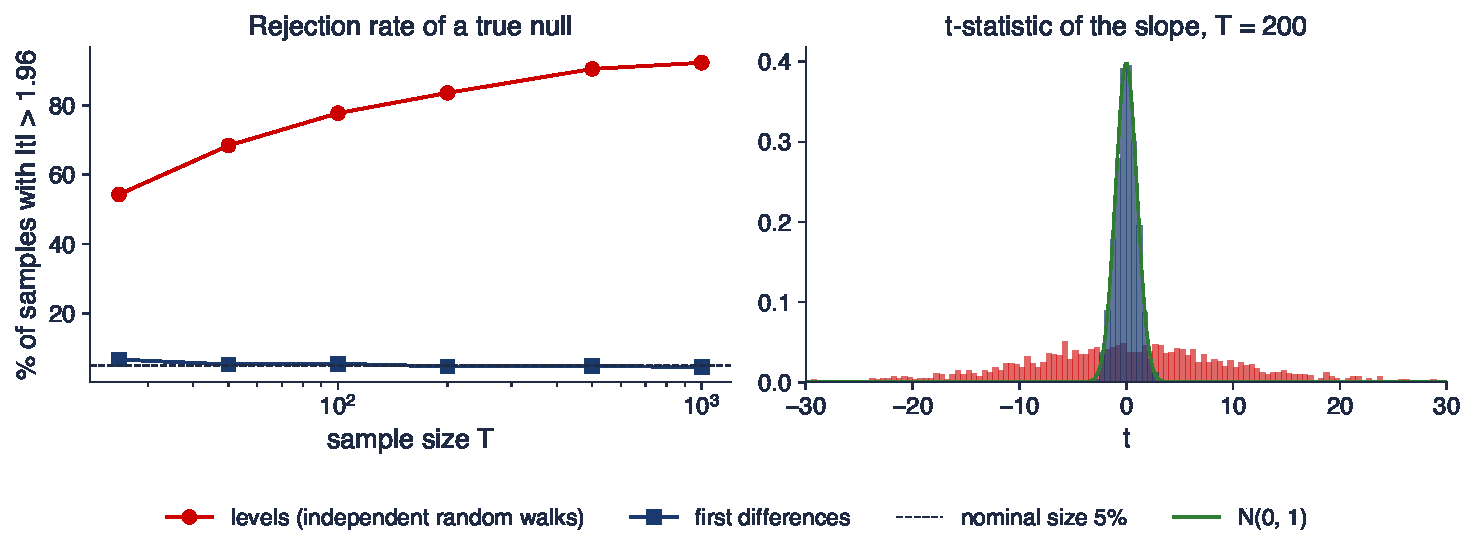
\includegraphics[width=0.97\textwidth,height=0.55\textheight,keepaspectratio]{tsa_ch3_spurious_mc.pdf}
\end{center}
\vspace{-0.25cm}
\begin{itemize}
    \item 2\,000 de perechi de mersuri aleatoare gaussiene independente pentru fiecare $T$; OLS a lui $y$ pe o constantă și pe $x$, în niveluri și în diferențe
    \item Stînga: proporția eșantioanelor cu $|t| > 1{,}96$; dreapta: distribuția lui $t$ pentru $T = 200$
\end{itemize}
\quantlet{TSA\_ch3\_spurious\_regression}{\qlurl{TSA_ch3_spurious_regression}}
\end{frame}

\begin{frame}{Interpretarea simulării}
\itemsize{\small}
\begin{itemize}
    \item Niveluri: ipoteza adevărată $b = 0$ este respinsă în 68\% din eșantioane cu $T = 50$ și în 92\% cu $T = 1000$
    \begin{itemize}
        \item mai multe date înrăutățesc situația: $|t|$ median crește de la 3{,}2 ($T = 50$) la 14{,}2 ($T = 1000$)
        \item $R^2$ median de circa 0{,}17 pentru orice $T$; DW median 0{,}08 la $T = 200$
    \end{itemize}
    \item Diferențe: 4{,}7\% la $T = 200$, aproape de nivelul nominal de 5\%
    \begin{itemize}
        \item testul $t$ funcționează din nou, deoarece $\Delta y_t$ și $\Delta x_t$ sînt staționare
    \end{itemize}
\end{itemize}
\end{frame}

\begin{frame}{Motivul pentru care testul $t$ eșuează}
\itemsize{\small}
\begin{itemize}
    \item În ipoteza $b = 0$, eroarea $e_t = y_t - a$ este ea însăși un mers aleator: ipotezele OLS (erori staționare, necorelate) nu sînt îndeplinite
    \begin{itemize}
        \item eroarea standard obișnuită este mult prea mică
    \end{itemize}
    \item \refPhillips\ a dedus comportamentul în eșantioane mari
    \begin{itemize}
        \item $\hat b$ nu converge la 0: converge la o variabilă aleatoare
        \item $t_{\hat b}$ crește ca $\sqrt{T}$, deci rata de respingere tinde la 100\%
        \item $R^2$ are o distribuție limită nedegenerată; $\mathrm{DW} \to 0$
    \end{itemize}
    \item Excepția: dacă $y_t - b x_t$ este staționar pentru un anumit $b$, seriile sînt \textbf{cointegrate}, iar regresia în niveluri are sens \refEG\ (\tsachlink{https://danpele.github.io/Time-Series-Analysis/RO/Cursuri/capitol7_cointegrare_vecm.pdf}{Capitolul 7})
\end{itemize}
\end{frame}

\begin{frame}{O regresie falsă pe date reale}
\itemsize{\footnotesize}
\begin{center}
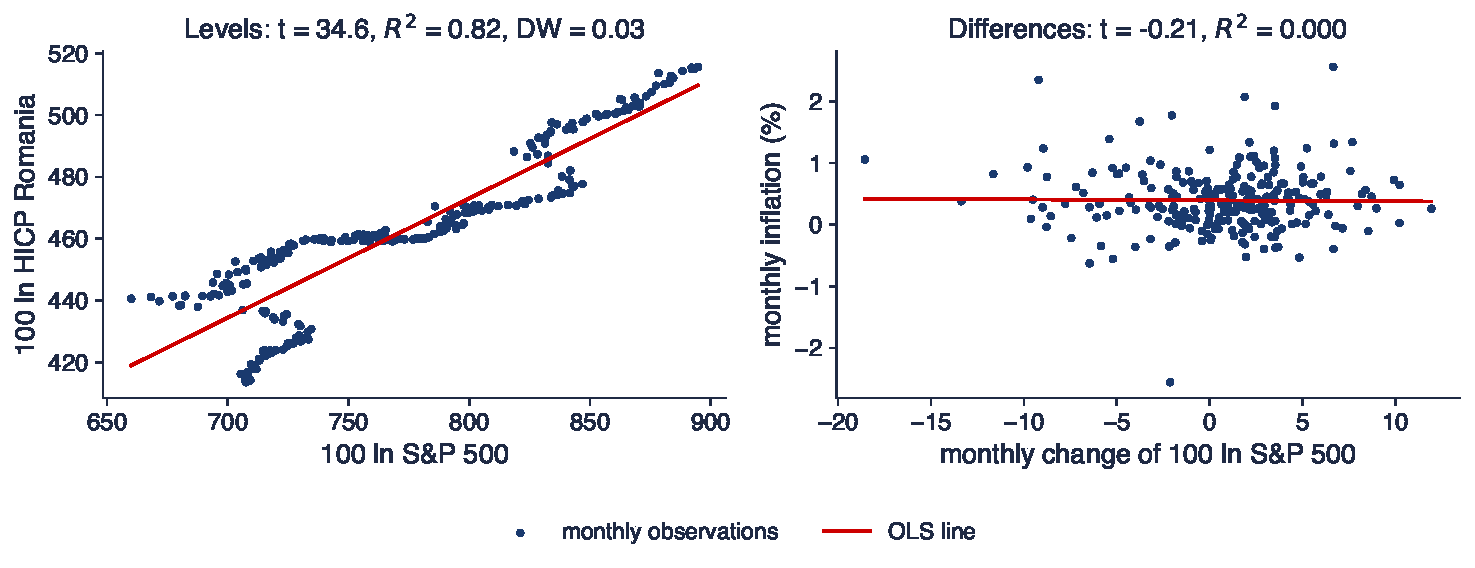
\includegraphics[width=0.97\textwidth,height=0.55\textheight,keepaspectratio]{tsa_ch3_spurious_real.pdf}
\end{center}
\vspace{-0.25cm}
\begin{itemize}
    \item IAPC al României (Eurostat) față de S\&P 500 (închiderea de la sfîrșitul lunii), 260 de luni din ianuarie 2005, ambele ca $100\ln$
    \item Stînga: niveluri; dreapta: variații lunare
\end{itemize}
\quantlet{TSA\_ch3\_spurious\_regression}{\qlurl{TSA_ch3_spurious_regression}}
\end{frame}

\begin{frame}{Interpretarea regresiei IAPC}
\itemsize{\small}
\begin{itemize}
    \item Niveluri: panta 0{,}39, $t = 34{,}6$, $R^2 = 0{,}82$, $\mathrm{DW} = 0{,}03$
    \begin{itemize}
        \item „Acțiunile americane explică prețurile de consum din România”: $R^2 > \mathrm{DW}$, o regresie falsă tipică
    \end{itemize}
    \item Diferențe: $t = \ensuremath{-}0{,}21$ (p = 0{,}83), $R^2 = 0{,}0002$
    \begin{itemize}
        \item inflația lunară și randamentul lunar al acțiunilor nu sînt legate
    \end{itemize}
    \item Ambele niveluri conțin un trend; regresia spune doar că ambele au crescut
\end{itemize}
\end{frame}

\begin{frame}{Recapitulare: regresia falsă}
\itemsize{\small}
\begin{itemize}
    \item Regresia unei serii $I(1)$ pe o altă serie $I(1)$ fără legătură cu ea dă un $t$ mare, un $R^2$ mare și un DW apropiat de 0
    \item Mai multe observații nu ajută: $t$ crește ca $\sqrt{T}$
    \item Remedii: testăm întîi ordinul de integrare; estimăm regresia pe diferențe; sau testăm cointegrarea (\tsachlink{https://danpele.github.io/Time-Series-Analysis/RO/Cursuri/capitol7_cointegrare_vecm.pdf}{Capitolul 7})
\end{itemize}
\end{frame}


%=============================================================================
\section{Testul Dickey--Fuller}
%=============================================================================

\begin{frame}{Testarea ipotezei $\phi = 1$}
\itemsize{\small}
\begin{itemize}
    \item AR(1): $y_t = \phi y_{t-1} + \varepsilon_t$; scădem $y_{t-1}$: $\Delta y_t = \gamma y_{t-1} + \varepsilon_t$, cu $\gamma = \phi - 1$
    \begin{itemize}
        \item $H_0$: $\gamma = 0$ (rădăcină unitară, $I(1)$); $H_1$: $\gamma < 0$ (staționar); un test unilateral, la stînga
        \item statistica: $\tau = \hat\gamma/\mathrm{SE}(\hat\gamma)$, raportul $t$ obișnuit din OLS; $\mathrm{SE}$: eroarea standard; un $\tau$ foarte negativ este un argument împotriva rădăcinii unitare
    \end{itemize}
    \item În ipoteza $H_0$, $\tau$ \textbf{nu} urmează legea Student sau distribuția Normală \refDF
    \begin{itemize}
        \item $y_{t-1}$ este un mers aleator, deci regresorul nu este staționar; $\hat\phi$ converge cu viteza $T$, nu $\sqrt{T}$ (\textbf{superconsistență})
        \item limita lui $\tau$ este o funcțională a mișcării browniene, asimetrică la stînga \refHamilton, cap.~17
        \item valorile critice provin din simulare: \refFuller; astăzi, din suprafețe de răspuns \refMacKinnonb
    \end{itemize}
\end{itemize}
\end{frame}

\begin{frame}{Iowa State: locul unde s-a născut testul}
\itemsize{\small}
\begin{columns}[T]
\begin{column}{0.48\textwidth}
\centering
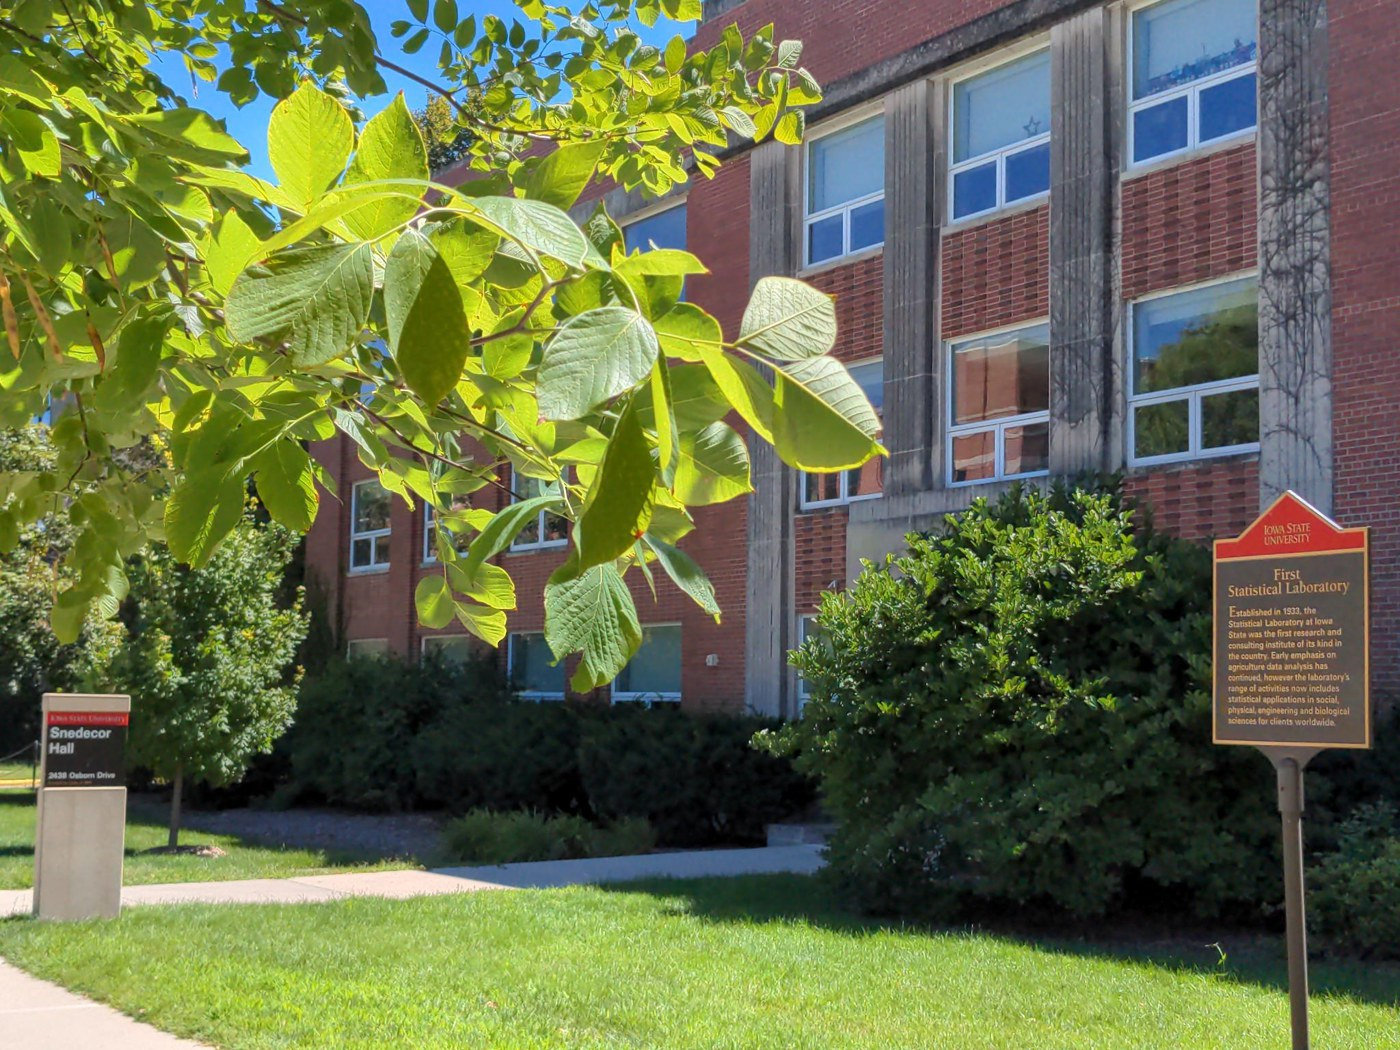
\includegraphics[height=0.44\textheight]{ch3_snedecor_hall_2023.jpg}\\[1mm]
\imgcap{Snedecor Hall, Iowa State University: departamentul de statistică și laboratorul său de statistică (1933)}
\imgcredit{https://commons.wikimedia.org/wiki/File:Snedecor_Hall,_Iowa_State_University.tif}{Foto: Maitra (2023); CC BY-SA 4.0; Wikimedia Commons}
\end{column}
\begin{column}{0.48\textwidth}
\begin{itemize}
    \item \textbf{Wayne A. Fuller}: statistician la Iowa State, autorul lucrării \textit{Introduction to Statistical Time Series} \refFuller
    \item \textbf{David A. Dickey}: doctorandul lui la Iowa State (1976), apoi la North Carolina State University
    \item \refDF: distribuția lui $\hat\phi$ și $\tau$ în cazul unei rădăcini unitare; \refDFb: teste comune pentru rădăcina unitară și termenii determiniști
    \item \refSD: testul augmentat pentru erori ARMA (în această secțiune)
\end{itemize}
\end{column}
\end{columns}
\end{frame}

\begin{frame}{Trei regresii Dickey--Fuller}
\itemsize{\small}
\begin{itemize}
    \item \textbf{Fără constantă}: $\Delta y_t = \gamma y_{t-1} + \varepsilon_t$
    \begin{itemize}
        \item $H_1$: staționar cu media 0; rareori realist
    \end{itemize}
    \item \textbf{Constantă}: $\Delta y_t = c + \gamma y_{t-1} + \varepsilon_t$
    \begin{itemize}
        \item $H_0$: mers aleator (cu derivă dacă $c \ne 0$); $H_1$: staționar în jurul unei medii nenule
        \item pentru serii fără trend: rate ale dobînzii, inflație, cursuri de schimb, randamente
    \end{itemize}
    \item \textbf{Constantă și trend}: $\Delta y_t = c + bt + \gamma y_{t-1} + \varepsilon_t$
    \begin{itemize}
        \item $c$: constanta; $bt$: un trend liniar cu panta $b$
        \item $H_0$: mers aleator cu derivă; $H_1$: staționar în jurul trendului: exact întrebarea din secțiunea 1
        \item pentru serii cu trend: logaritmul PIB, logaritmii prețurilor, logaritmii indicilor de preț
    \end{itemize}
    \item Fiecare caz are propria distribuție a lui $\tau$ și propriile valori critice
\end{itemize}
\end{frame}

\begin{frame}{Distribuțiile Dickey--Fuller}
\itemsize{\footnotesize}
\begin{center}
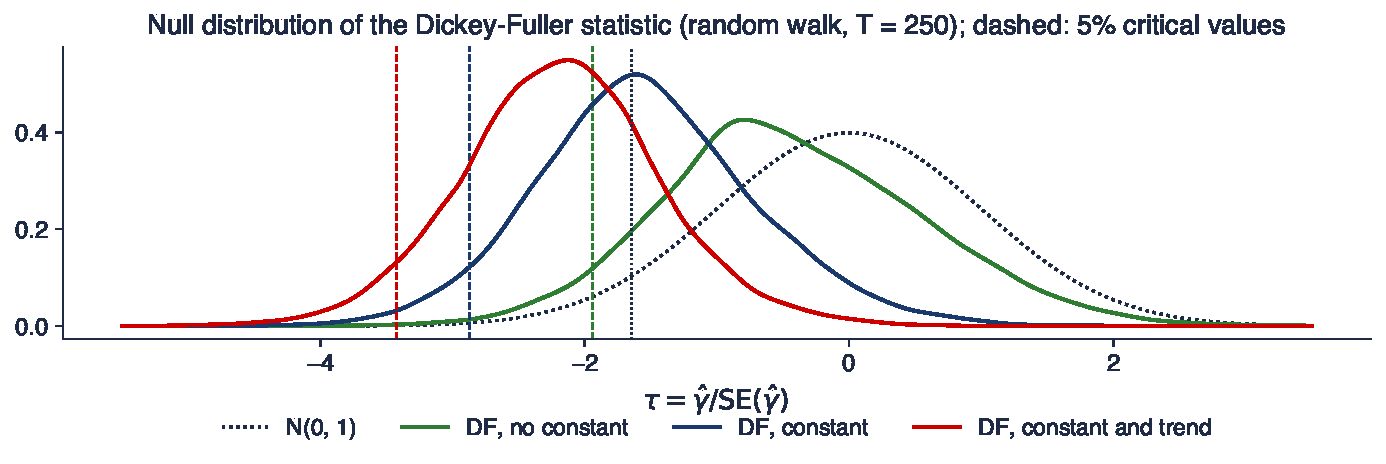
\includegraphics[width=0.97\textwidth,height=0.56\textheight,keepaspectratio]{tsa_ch3_df_dist.pdf}
\end{center}
\vspace{-0.25cm}
\begin{itemize}
    \item 20\,000 de mersuri aleatoare cu $T = 250$: densitatea lui $\tau$ în cele trei regresii, față de $N(0, 1)$; liniile întrerupte: valorile critice de 5\% \refMacKinnonb
\end{itemize}
\quantlet{TSA\_ch3\_dickey\_fuller}{\qlurl{TSA_ch3_dickey_fuller}}
\end{frame}

\begin{frame}{Interpretarea celor trei distribuții}
\itemsize{\small}
\begin{itemize}
    \item Toate trei sînt la stînga lui $N(0, 1)$; cu cît sînt mai mulți termeni determiniști, cu atît mai la stînga
    \begin{itemize}
        \item cuantilele de 5\% simulate: $\ensuremath{-}1{,}95$ (fără constantă), $\ensuremath{-}2{,}86$ (constantă) și $\ensuremath{-}3{,}42$ (constantă și trend); valorile din tabele: $\ensuremath{-}1{,}94$; $\ensuremath{-}2{,}87$ și $\ensuremath{-}3{,}43$
    \end{itemize}
    \item Cu valoarea critică a distribuției Normale, $-1{,}645$, o rădăcină unitară adevărată este „respinsă” în 46\% din eșantioane (constantă) și în 77\% (constantă și trend)
    \begin{itemize}
        \item tabelul greșit transformă mersurile aleatoare în serii „staționare”
    \end{itemize}
\end{itemize}
\end{frame}

\begin{frame}{Valorile critice ale testului Dickey--Fuller}
\itemsize{\small}
\begin{center}
\scriptsize
\begin{tabular}{lccc|ccc|ccc}
\toprule
& \multicolumn{3}{c|}{\textbf{fără constantă}} & \multicolumn{3}{c|}{\textbf{constantă}} & \multicolumn{3}{c}{\textbf{constantă și trend}} \\ $T$ & 1\% & 5\% & 10\% & 1\% & 5\% & 10\% & 1\% & 5\% & 10\% \\
\midrule
50 & $\ensuremath{-}2{,}61$ & $\ensuremath{-}1{,}95$ & $\ensuremath{-}1{,}61$ & $\ensuremath{-}3{,}57$ & $\ensuremath{-}2{,}92$ & $\ensuremath{-}2{,}60$ & $\ensuremath{-}4{,}15$ & $\ensuremath{-}3{,}50$ & $\ensuremath{-}3{,}18$ \\
100 & $\ensuremath{-}2{,}59$ & $\ensuremath{-}1{,}94$ & $\ensuremath{-}1{,}61$ & $\ensuremath{-}3{,}50$ & $\ensuremath{-}2{,}89$ & $\ensuremath{-}2{,}58$ & $\ensuremath{-}4{,}05$ & $\ensuremath{-}3{,}46$ & $\ensuremath{-}3{,}15$ \\
250 & $\ensuremath{-}2{,}57$ & $\ensuremath{-}1{,}94$ & $\ensuremath{-}1{,}62$ & $\ensuremath{-}3{,}46$ & $\ensuremath{-}2{,}87$ & $\ensuremath{-}2{,}57$ & $\ensuremath{-}4{,}00$ & $\ensuremath{-}3{,}43$ & $\ensuremath{-}3{,}14$ \\
$\infty$ & $\ensuremath{-}2{,}57$ & $\ensuremath{-}1{,}94$ & $\ensuremath{-}1{,}62$ & $\ensuremath{-}3{,}43$ & $\ensuremath{-}2{,}86$ & $\ensuremath{-}2{,}57$ & $\ensuremath{-}3{,}96$ & $\ensuremath{-}3{,}41$ & $\ensuremath{-}3{,}13$ \\
\bottomrule
\end{tabular}
\end{center}
\begin{itemize}
    \item Sursa: suprafețele de răspuns din \refMacKinnonb, folosite de \texttt{statsmodels}; p-value-urile din \refMacKinnon
    \item Decizia: respingem rădăcina unitară la 5\% dacă $\tau$ este \textbf{sub} (mai negativ decît) valoarea de 5\%
    \item Valorile depind puțin de $T$; se aplică neschimbate testului ADF
\end{itemize}
\end{frame}

\begin{frame}{Exemplu rezolvat: PIB-ul real al României}
\itemsize{\small}
\begin{itemize}
    \item $y_t = 100\ln$ PIB real, T1 2000--T2 2026; regresia cu constantă și trend, fără laguri ($T = 105$ diferențe)
    \begin{itemize}
        \item OLS: $\hat\gamma = \ensuremath{-}0{,}0961$, $\mathrm{SE}(\hat\gamma) = 0{,}0416$, deci $\hat\phi = 1 + \hat\gamma = 0{,}904$
    \end{itemize}
    \item $\tau = \ensuremath{-}0{,}0961/0{,}0416 = \ensuremath{-}2{,}31$; valoarea critică de 5\% cu constantă și trend: $\ensuremath{-}3{,}45$
    \begin{itemize}
        \item $\ensuremath{-}2{,}31 > \ensuremath{-}3{,}45$: nu respingem rădăcina unitară (p = 0{,}43)
        \item cu valoarea distribuției Normale, $-1{,}645$, am fi respins-o: tabelul greșit dă răspunsul greșit
    \end{itemize}
    \item Interpretarea: „nerespins” nu înseamnă „demonstrat”
    \begin{itemize}
        \item dacă $\phi = 0{,}904$ ar fi adevărat, un șoc s-ar înjumătăți în $\ln 0{,}5/\ln 0{,}904 \approx 6{,}9$ trimestre; cu 106 observații, testul abia poate deosebi această situație de $\phi = 1$
    \end{itemize}
\end{itemize}
\end{frame}

\begin{frame}{Testul Dickey--Fuller augmentat}
\itemsize{\small}
\begin{itemize}
    \item Dacă $\Delta y_t$ este autocorelat, $\varepsilon_t$ din regresia DF nu este zgomot alb, iar mărimea testului este greșită
    \begin{itemize}
        \item remediul: adăugăm diferențele trecute $\Delta y_{t-j}$
    \end{itemize}
    \item Regresia \textbf{ADF} (augmented Dickey--Fuller, Dickey--Fuller augmentat):
    \begin{itemize}
        \item $\Delta y_t = c + bt + \gamma y_{t-1} + \sum_{j=1}^{k} \delta_j \Delta y_{t-j} + \varepsilon_t$; același $\tau$, aceleași valori critice
        \item $\delta_j$: coeficienții diferențelor trecute; $k$: numărul de diferențe trecute incluse (lagurile)
        \item un AR($p$) în niveluri devine exact această regresie, cu $k = p - 1$ și $\gamma = -\phi(1)$
    \end{itemize}
    \item \refSD: cu erori ARMA, testul rămîne valid dacă $k$ crește încet odată cu $T$
    \begin{itemize}
        \item lagurile aproximează partea MA printr-un AR lung
    \end{itemize}
    \item Testul ADF este testul implicit de rădăcină unitară în programe: \texttt{adfuller} în \texttt{statsmodels}
\end{itemize}
\end{frame}

\begin{frame}{Alegerea numărului de laguri $k$}
\itemsize{\small}
\begin{itemize}
    \item Maximul: $k_{\max} = 12\,(T/100)^{1/4}$ \refSchwert; pentru $T = 105$, $k_{\max} = 13$
    \begin{itemize}
        \item apoi alegem $k \le k_{\max}$ după un criteriu informațional, AIC sau BIC (\tsachlink{https://danpele.github.io/Time-Series-Analysis/RO/Cursuri/capitol2_modele_arma.pdf}{Capitolul 2}), pe același eșantion pentru fiecare $k$
    \end{itemize}
    \item Prea puține laguri: erori autocorelate, mărime greșită (cu o componentă MA negativă, mult prea multe respingeri)
    \begin{itemize}
        \item prea multe laguri: putere mai mică
    \end{itemize}
    \item \refNgP: un AIC modificat (MAIC) dă o mărime mai bună; eliminarea trendului prin GLS \refERS\ dă mai multă putere
    \begin{itemize}
        \item MAIC: modified Akaike information criterion (criteriul Akaike modificat); GLS: generalised least squares (metoda generalizată a celor mai mici pătrate); ambele apar în testul DF-GLS
    \end{itemize}
    \item Verificăm rezultatul: testul Ljung--Box pe reziduurile ADF \refLB; raportăm $k$ împreună cu $\tau$
\end{itemize}
\end{frame}

\begin{frame}{Mărimea și puterea testului Dickey--Fuller}
\itemsize{\footnotesize}
\begin{center}
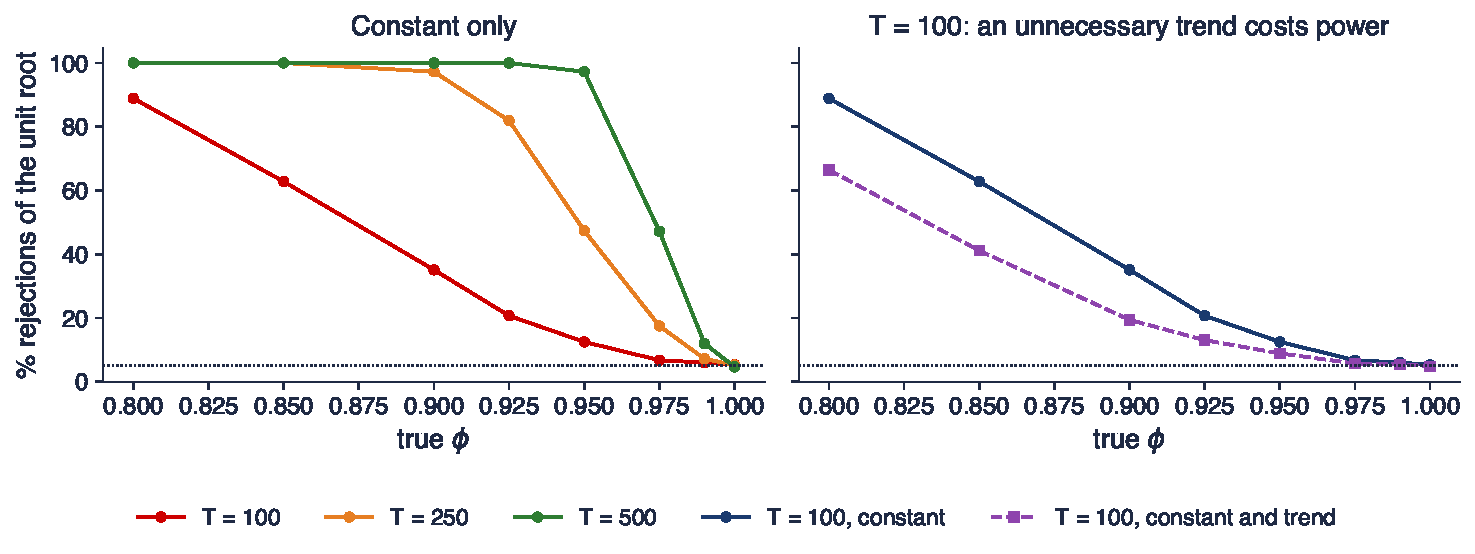
\includegraphics[width=0.97\textwidth,height=0.55\textheight,keepaspectratio]{tsa_ch3_adf_power.pdf}
\end{center}
\vspace{-0.25cm}
\begin{itemize}
    \item 2\,000 de traiectorii AR(1) $y_t = \phi y_{t-1} + \varepsilon_t$ pentru fiecare $\phi$; proporția respingerilor la 5\%; la $\phi = 1$ aceasta este mărimea testului
\end{itemize}
\quantlet{TSA\_ch3\_dickey\_fuller}{\qlurl{TSA_ch3_dickey_fuller}}
\end{frame}

\begin{frame}{Interpretarea curbelor de putere}
\itemsize{\small}
\begin{itemize}
    \item Mărimea: 5\%, 5\% și 5\% la $\phi = 1$: testul își respectă nivelul de 5\%
    \item Puterea la $\phi = 0{,}95$: 12\% cu $T = 100$, 47\% cu $T = 250$, 97\% cu $T = 500$
    \begin{itemize}
        \item o serie trimestrială de 25 de ani ($T = 100$) aproape niciodată nu deosebește $\phi = 0{,}95$ de o rădăcină unitară
        \item contează lungimea perioadei, nu frecvența: datele zilnice pe doi ani nu ajută
    \end{itemize}
    \item Un trend inutil costă putere: la $T = 100$ și $\phi = 0{,}9$, 35\% cu constantă, 19\% cu constantă și trend
\end{itemize}
\end{frame}

\begin{frame}{Alegerea termenilor determiniști}
\itemsize{\small}
\begin{itemize}
    \item Ipoteza alternativă trebuie să fie o descriere plauzibilă a datelor
    \begin{itemize}
        \item serii cu trend (logaritmul PIB, logaritmii prețurilor): constantă și trend
        \item serii care fluctuează în jurul unui nivel (rate ale dobînzii, inflație, cursuri de schimb, randamente): constantă
    \end{itemize}
    \item Omiterea unui trend necesar: o serie staționară în jurul trendului pare să aibă rădăcină unitară; testul aproape niciodată nu respinge
    \begin{itemize}
        \item adăugarea unui trend inutil: putere mai mică (graficul anterior)
    \end{itemize}
    \item Ne uităm întîi la grafic, apoi alegem; \refDFb\ propun teste comune de tip $F$ pentru rădăcina unitară și trend
\end{itemize}
\end{frame}

\begin{frame}{Cîte diferențieri: $I(1)$ sau $I(2)$?}
\itemsize{\small}
\begin{itemize}
    \item \refDP: testăm de la cel mai mare ordin plauzibil în jos
    \begin{itemize}
        \item pasul 1: ADF pe $\Delta y_t$; dacă nu respinge, $y_t$ poate fi $I(2)$
        \item pasul 2: dacă respinge, ADF pe $y_t$; respingere: $I(0)$; nerespingere: $I(1)$
    \end{itemize}
    \item Motivul ordinii descendente: dacă $y_t \sim I(2)$, testul pe $y_t$ presupune cel mult o rădăcină unitară și nu este valid
    \item Exemplu: prețurile de consum din România după 2005 (tabelul din secțiunea 4)
    \begin{itemize}
        \item $\ln P$: rădăcină unitară; inflația $\pi$: ADF p = 0{,}32, KPSS 0{,}404; variația inflației: clar staționară
        \item deci $\ln P$ este $I(1)$ sau $I(2)$, în funcție de cît de persistentă este inflația: secțiunea 7 revine asupra acestei întrebări
    \end{itemize}
\end{itemize}
\end{frame}

\begin{frame}{Recapitulare: testul Dickey--Fuller}
\itemsize{\small}
\begin{itemize}
    \item $\Delta y_t = c + bt + \gamma y_{t-1} + \sum_j\delta_j\Delta y_{t-j} + \varepsilon_t$; $H_0$: $\gamma = 0$; $\tau$ comparat cu valorile critice Dickey--Fuller
    \item Termenii determiniști urmează graficul; lagurile se aleg după AIC sau BIC, pînă la $12(T/100)^{1/4}$
    \item Putere mică în apropierea lui $\phi = 1$: nerespingerea este o dovadă slabă în favoarea rădăcinii unitare
    \item Ordinul de integrare: testăm de sus în jos (întîi $\Delta y_t$)
\end{itemize}
\end{frame}


%=============================================================================
\section{Phillips--Perron, KPSS și folosirea lor împreună}
%=============================================================================

\begin{frame}{Testul Phillips--Perron}
\itemsize{\small}
\begin{itemize}
    \item \refPP: păstrăm regresia DF simplă (fără diferențele trecute) și corectăm în schimb statistica $\tau$
    \begin{itemize}
        \item $Z_\tau = \sqrt{\hat\gamma_0/\hat\lambda^2}\;\tau - \dfrac{(\hat\lambda^2 - \hat\gamma_0)\,T\,\mathrm{SE}(\hat\gamma)}{2\hat\lambda\,s}$
        \item $\hat\gamma_0$: varianța reziduurilor; $s^2$: varianța lor OLS; $\hat\lambda^2$: \textbf{varianța lor pe termen lung}
    \end{itemize}
    \item Varianța pe termen lung (Newey--West, ponderi Bartlett): $\hat\lambda^2 = \hat\gamma_0 + 2\sum_{j=1}^{L}(1 - \frac{j}{L+1})\hat\gamma_j$
    \begin{itemize}
        \item $\hat\gamma_j$: autocovarianțele reziduurilor; $L$: numărul de autocovarianțe incluse (lățimea de bandă)
        \item dacă reziduurile sînt zgomot alb, $\hat\lambda^2 = \hat\gamma_0$ și $Z_\tau = \tau$: corecția contează doar cînd ele sînt autocorelate
    \end{itemize}
    \item Aceeași $H_0$ și aceleași valori critice ca ADF; robust la heteroscedasticitate; nu alegem laguri, ci o lățime de bandă $L$
    \begin{itemize}
        \item punctul slab: distorsiuni mari ale mărimii cînd există o componentă MA negativă \refSchwert
    \end{itemize}
\end{itemize}
\end{frame}

\begin{frame}{Testul KPSS: staționaritatea ca ipoteză nulă}
\itemsize{\small}
\begin{itemize}
    \item \refKPSS\ (KPSS: Kwiatkowski--Phillips--Schmidt--Shin): $y_t = \xi t + r_t + \varepsilon_t$, $r_t = r_{t-1} + u_t$, $u_t \sim \mathrm{WN}(0, \sigma_u^2)$
    \begin{itemize}
        \item $\xi t$: un trend determinist; $r_t$: un mers aleator, adică nivelul care se deplasează; $\varepsilon_t$: zgomot staționar
        \item $H_0$: $\sigma_u^2 = 0$ (mersul aleator este o constantă: $y_t$ staționar în jurul unui nivel sau al unui trend); $H_1$: $\sigma_u^2 > 0$, o rădăcină unitară
    \end{itemize}
    \item Statistica: regresia lui $y_t$ pe o constantă (și un trend); reziduurile $e_t$; sumele parțiale $S_t = e_1 + \dots + e_t$
    \begin{itemize}
        \item $\eta = \dfrac{1}{T^2\hat\lambda^2}\sum_{t=1}^{T} S_t^2$, unde $\hat\lambda^2$ este varianța pe termen lung a lui $e_t$
        \item respingem staționaritatea pentru valori \textbf{mari} ale lui $\eta$: valorile critice de 5\% sînt 0,463 (nivel) și 0,146 (trend); la 1\%: 0,739 și 0,216
    \end{itemize}
    \item Un test al staționarității, nu al rădăcinii unitare: inversează sarcina probei
\end{itemize}
\end{frame}

\begin{frame}{KPSS: rolul sumelor parțiale}
\itemsize{\footnotesize}
\begin{center}
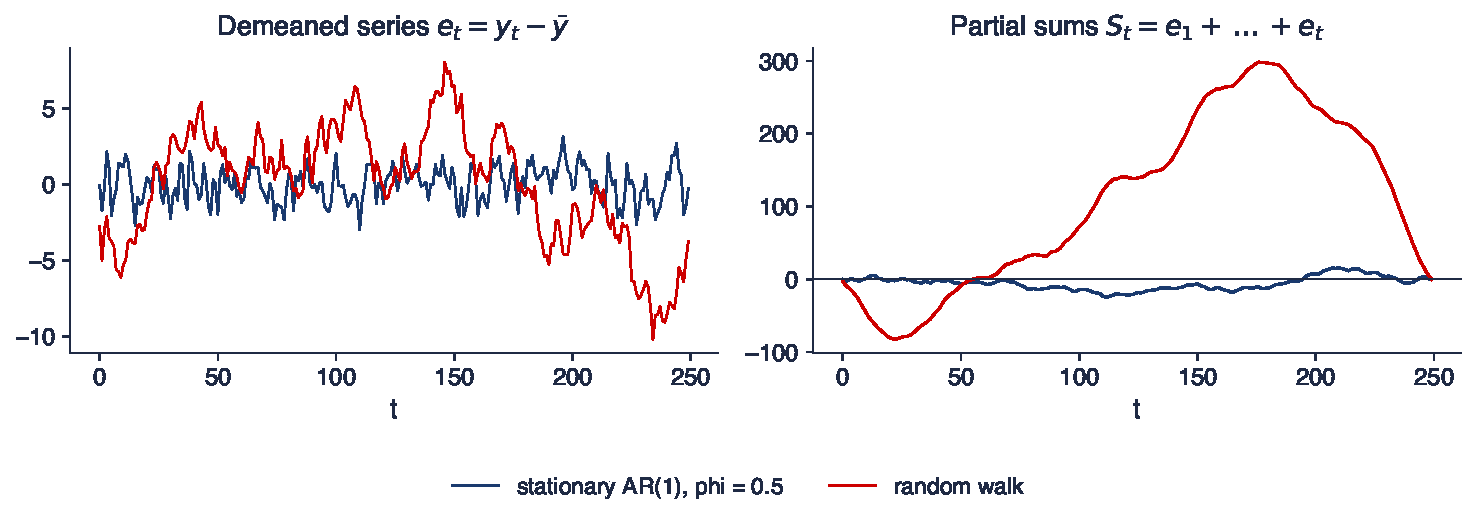
\includegraphics[width=0.97\textwidth,height=0.52\textheight,keepaspectratio]{tsa_ch3_kpss_sums.pdf}
\end{center}
\vspace{-0.25cm}
\begin{itemize}
    \item Un AR(1) staționar ($\phi = 0{,}5$) și un mers aleator, $T = 250$: seriile centrate și sumele lor parțiale $S_t$
    \item KPSS (nivel): 0{,}16 pentru AR(1), 0{,}73 pentru mersul aleator; valoarea critică de 5\% este 0,463
\end{itemize}
\quantlet{TSA\_ch3\_unit\_root\_tests}{\qlurl{TSA_ch3_unit_root_tests}}
\end{frame}

\begin{frame}{Interpretarea sumelor parțiale}
\itemsize{\small}
\begin{itemize}
    \item Seria staționară: abaterile se compensează, $S_t$ rămîne aproape de 0
    \begin{itemize}
        \item $\sum S_t^2$ crește ca $T^2$, deci $\eta$ rămîne mărginit
    \end{itemize}
    \item Mersul aleator: perioade lungi de o parte a mediei, $S_t$ se abate mult de la 0
    \begin{itemize}
        \item $\sum S_t^2$ crește ca $T^4$: $\eta$ crește cu $T$, iar testul respinge
    \end{itemize}
    \item Aceeași idee ca în graficele CUSUM din controlul calității: abaterile cumulate dezvăluie un nivel care se deplasează
\end{itemize}
\end{frame}

\begin{frame}{ADF și KPSS împreună}
\itemsize{\small}
\begin{center}
\footnotesize
\begin{tabular}{lll}
\toprule
& \textbf{KPSS nu respinge} & \textbf{KPSS respinge} \\
\midrule
\textbf{ADF respinge} & $I(0)$: ambele concordă & conflict: ruptură, memorie lungă, valori extreme? \\
\textbf{ADF nu respinge} & neconcludent: datele nu pot decide & $I(1)$: ambele concordă \\
\bottomrule
\end{tabular}
\end{center}
\begin{itemize}
    \item Cele două teste au ipoteze nule opuse: concordanța lor este o dovadă mai puternică decît oricare test singur
    \item Situația neconcludentă este frecventă în eșantioane scurte: putere mică de ambele părți
    \begin{itemize}
        \item atunci decidem după scop: pentru prognoză, $d = 1$ este alegerea prudentă (intervale mai largi)
    \end{itemize}
    \item Conflict: căutăm rupturi (secțiunea 5) sau integrare fracționară (\tsachlink{https://danpele.github.io/Time-Series-Analysis/RO/Cursuri/capitol8_memorie_lunga_arfima.pdf}{Capitolul 8})
\end{itemize}
\end{frame}

\begin{frame}{Teste de rădăcină unitară pe serii reale}
\itemsize{\scriptsize}
\begin{center}
\scriptsize
\begin{tabular}{llrrrrrl}
\toprule
\textbf{Seria} & \textbf{det.} & $T$ & \textbf{ADF} (p) & $k$ & \textbf{PP} & \textbf{KPSS} & \textbf{ADF+KPSS} \\
\midrule
România, PIB real, $100\ln Y$ & c, t & 106 & $\ensuremath{-}2{,}31$ (0{,}428) & 0 & $\ensuremath{-}2{,}19$ & 0{,}198 & $I(1)$ \\
\quad creșterea $\Delta$ & c & 105 & $\ensuremath{-}10{,}77$ ($<$\,0{,}001) & 0 & $\ensuremath{-}10{,}88$ & 0{,}263 & $I(0)$ \\
România, IAPC, $100\ln P$ & c, t & 260 & $\ensuremath{-}0{,}96$ (0{,}949) & 6 & $\ensuremath{-}0{,}88$ & 0{,}314 & $I(1)$ \\
România, inflația anuală $\pi$ & c & 260 & $\ensuremath{-}1{,}94$ (0{,}315) & 15 & $\ensuremath{-}2{,}31$ & 0{,}404 & neconcludent \\
\quad variația $\Delta\pi$ & c & 259 & $\ensuremath{-}4{,}83$ ($<$\,0{,}001) & 14 & $\ensuremath{-}11{,}31$ & 0{,}105 & $I(0)$ \\
SUA, PIB real, $100\ln Y$ & c, t & 318 & $\ensuremath{-}1{,}54$ (0{,}816) & 1 & $\ensuremath{-}1{,}20$ & 0{,}581 & $I(1)$ \\
\quad creșterea $\Delta$ & c & 317 & $\ensuremath{-}15{,}51$ ($<$\,0{,}001) & 0 & $\ensuremath{-}15{,}44$ & 0{,}456 & $I(0)$ \\
EUR/RON, $100\ln S$ & c & 5\,353 & $\ensuremath{-}1{,}22$ (0{,}664) & 7 & $\ensuremath{-}1{,}15$ & 10{,}255 & $I(1)$ \\
\quad randamente zilnice & c & 5\,352 & $\ensuremath{-}27{,}42$ ($<$\,0{,}001) & 6 & $\ensuremath{-}60{,}82$ & 0{,}055 & $I(0)$ \\
BET, $100\ln P$ & c, t & 6\,671 & $\ensuremath{-}1{,}90$ (0{,}653) & 19 & $\ensuremath{-}2{,}35$ & 1{,}143 & $I(1)$ \\
\quad randamente zilnice & c & 6\,670 & $\ensuremath{-}16{,}50$ ($<$\,0{,}001) & 18 & $\ensuremath{-}74{,}55$ & 0{,}360 & $I(0)$ \\
S\&P 500, $100\ln P$ & c, t & 6\,715 & $\ensuremath{-}2{,}08$ (0{,}557) & 34 & $\ensuremath{-}2{,}36$ & 2{,}281 & $I(1)$ \\
\quad randamente zilnice & c & 6\,714 & $\ensuremath{-}14{,}26$ ($<$\,0{,}001) & 35 & $\ensuremath{-}91{,}41$ & 0{,}449 & $I(0)$ \\
Nilul, debitul anual & c & 100 & $\ensuremath{-}4{,}05$ (0{,}001) & 1 & $\ensuremath{-}6{,}38$ & 0{,}869 & conflict \\
\bottomrule
\end{tabular}
\end{center}
\begin{itemize}
    \item det.: termenii determiniști (c: constantă; t: trend); $k$: lagurile ADF (AIC); valori critice de 5\%: ADF și PP circa $-2{,}86$ (c), $-3{,}41$ (c, t); KPSS 0,463 (c), 0,146 (c, t)
\end{itemize}\quantlet{TSA\_ch3\_unit\_root\_tests}{\qlurl{TSA_ch3_unit_root_tests}}
\end{frame}

\begin{frame}{Interpretarea tabelului testelor}
\itemsize{\small}
\begin{itemize}
    \item Logaritmii prețurilor, cursul de schimb, logaritmul PIB și al IAPC: $I(1)$; diferențele lor: $I(0)$
    \begin{itemize}
        \item PIB-ul României: ADF p = 0{,}43 și KPSS 0{,}198 $> 0{,}146$: rădăcină unitară, cum au găsit \refNP\ pentru SUA
    \end{itemize}
    \item Inflația anuală din România: niciun test nu respinge (KPSS 0{,}404 $< 0{,}463$): neconcludent
    \begin{itemize}
        \item o serie foarte persistentă, posibil cu rupturi; secțiunile 5 și 7
    \end{itemize}
    \item Nilul: ambele resping: un conflict
    \begin{itemize}
        \item \tsachlink{https://danpele.github.io/Time-Series-Analysis/RO/Cursuri/capitol1_procese_stochastice_stationaritate.pdf}{Capitolul 1} a arătat o schimbare de nivel în 1898: secțiunea următoare explică acest conflict
    \end{itemize}
    \item Randamentele zilnice: PP dă valori mult mai negative decît ADF (BET: $\ensuremath{-}74{,}6$ față de $\ensuremath{-}16{,}5$), dar ambele resping; verdictul este același
\end{itemize}
\end{frame}

\begin{frame}{Recapitulare: Phillips--Perron și KPSS}
\itemsize{\small}
\begin{itemize}
    \item PP: regresia DF plus o corecție prin varianța pe termen lung; aceeași $H_0$ și aceleași valori critice ca ADF
    \item KPSS: $H_0$ este staționaritatea; sumele parțiale mari o resping
    \item Interpretăm ADF și KPSS împreună: concordanță, rezultat neconcludent sau conflict
\end{itemize}
\end{frame}


%=============================================================================
\section{Rupturi structurale}
%=============================================================================

\begin{frame}{Perron (1989): o ruptură poate semăna cu o rădăcină unitară}
\itemsize{\small}
\begin{itemize}
    \item \refPerron: o serie staționară în jurul unei medii sau al unui trend care \textbf{se schimbă o dată} pare persistentă
    \begin{itemize}
        \item regresia DF explică schimbarea printr-un $\hat\phi$ apropiat de 1; testul își pierde puterea
    \end{itemize}
    \item A reexaminat seriile Nelson și Plosser cu două rupturi cunoscute: crahul din 1929 (nivel) și șocul petrolier din 1973 (pantă)
    \begin{itemize}
        \item cu variabile dummy pentru ruptură, rădăcina unitară a fost respinsă pentru majoritatea seriilor
        \item interpretarea: majoritatea șocurilor sînt temporare; doar cîteva evenimente rare sînt permanente
    \end{itemize}
    \item Critica: data rupturii a fost aleasă după ce s-au văzut datele
\end{itemize}
\end{frame}

\begin{frame}{O schimbare de nivel înșală testul ADF}
\itemsize{\footnotesize}
\begin{center}
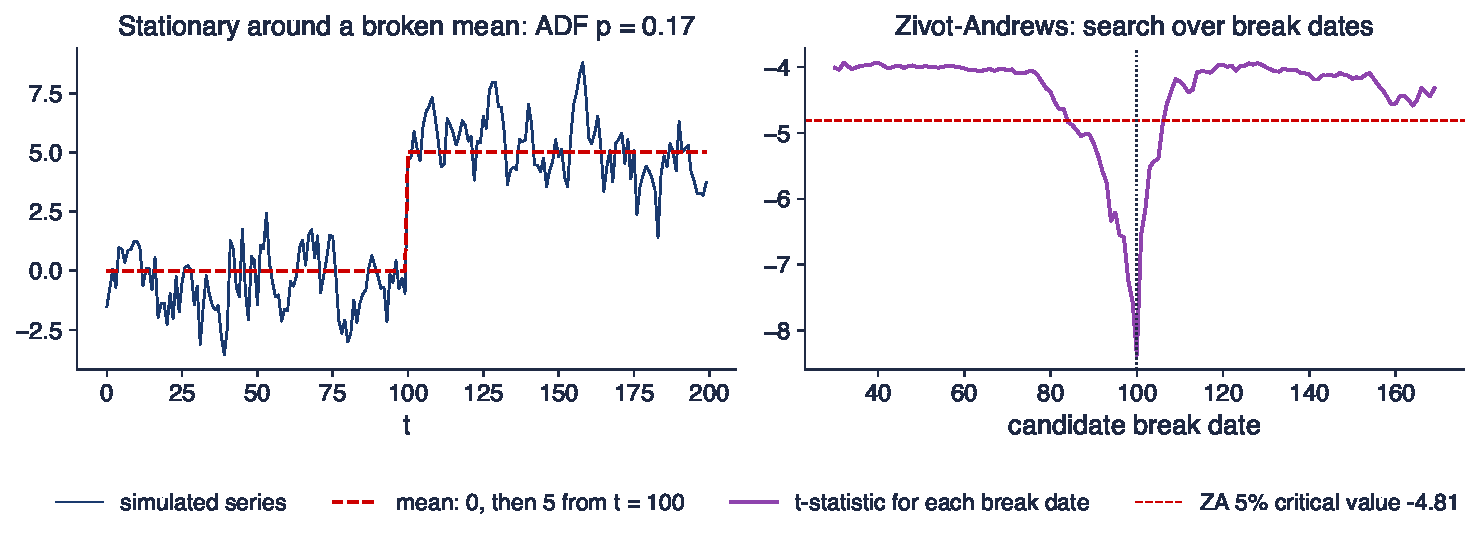
\includegraphics[width=0.97\textwidth,height=0.54\textheight,keepaspectratio]{tsa_ch3_breaks_sim.pdf}
\end{center}
\vspace{-0.25cm}
\begin{itemize}
    \item Stînga: zgomot AR(1) ($\phi = 0{,}6$) în jurul unei medii care sare de la 0 la 5 la $t = 100$; dreapta: statistica $t$ a lui $y_{t-1}$ pentru fiecare dată posibilă a rupturii, cu o variabilă dummy de nivel
\end{itemize}
\quantlet{TSA\_ch3\_structural\_breaks}{\qlurl{TSA_ch3_structural_breaks}}
\end{frame}

\begin{frame}{Interpretarea rupturii simulate}
\itemsize{\small}
\begin{itemize}
    \item ADF cu constantă: p = 0{,}17: seria staționară „are rădăcină unitară”
    \begin{itemize}
        \item pe 2\,000 de asemenea serii, testul DF respinge în 72\% din cazuri; fără ruptură: 100\%
    \end{itemize}
    \item Cînd ruptura este modelată, statistica scade la $\ensuremath{-}7{,}47$, mult sub valoarea de 5\%, $\ensuremath{-}4{,}81$
    \begin{itemize}
        \item minimul este atins la data adevărată, $t = 100$
    \end{itemize}
\end{itemize}
\end{frame}

\begin{frame}{Zivot și Andrews (1992): data rupturii necunoscută}
\itemsize{\small}
\begin{itemize}
    \item \refZA: lăsăm datele să aleagă data rupturii $T_B$
    \begin{itemize}
        \item pentru fiecare $T_B$ din cele 70\% centrale ale eșantionului, estimăm regresia ADF cu o variabilă dummy pentru ruptură:
        \item $\Delta y_t = c + \theta DU_t + bt + \gamma y_{t-1} + \sum_j\delta_j\Delta y_{t-j} + \varepsilon_t$, $DU_t = 1$ pentru $t > T_B$
        \item $DU_t$: o variabilă dummy, 0 înainte și 1 după ruptură; $\theta$: mărimea saltului de nivel
        \item statistica este raportul $t$ \textbf{minim} al lui $\gamma$ pe toate datele
    \end{itemize}
    \item Trei variante: ruptură în nivel, în pantă sau în ambele
    \begin{itemize}
        \item valori critice mai negative decît la ADF: circa $-4{,}81$ (nivel) și $-5{,}07$ (ambele) la 5\%
    \end{itemize}
    \item $H_0$: rădăcină unitară fără ruptură; $H_1$: staționar cu o ruptură
    \begin{itemize}
        \item mai multe rupturi: \refBaiP; o respingere nu demonstrează că ruptura este explicația corectă
    \end{itemize}
\end{itemize}
\end{frame}

\begin{frame}{Zivot--Andrews pe două serii reale}
\itemsize{\footnotesize}
\begin{center}
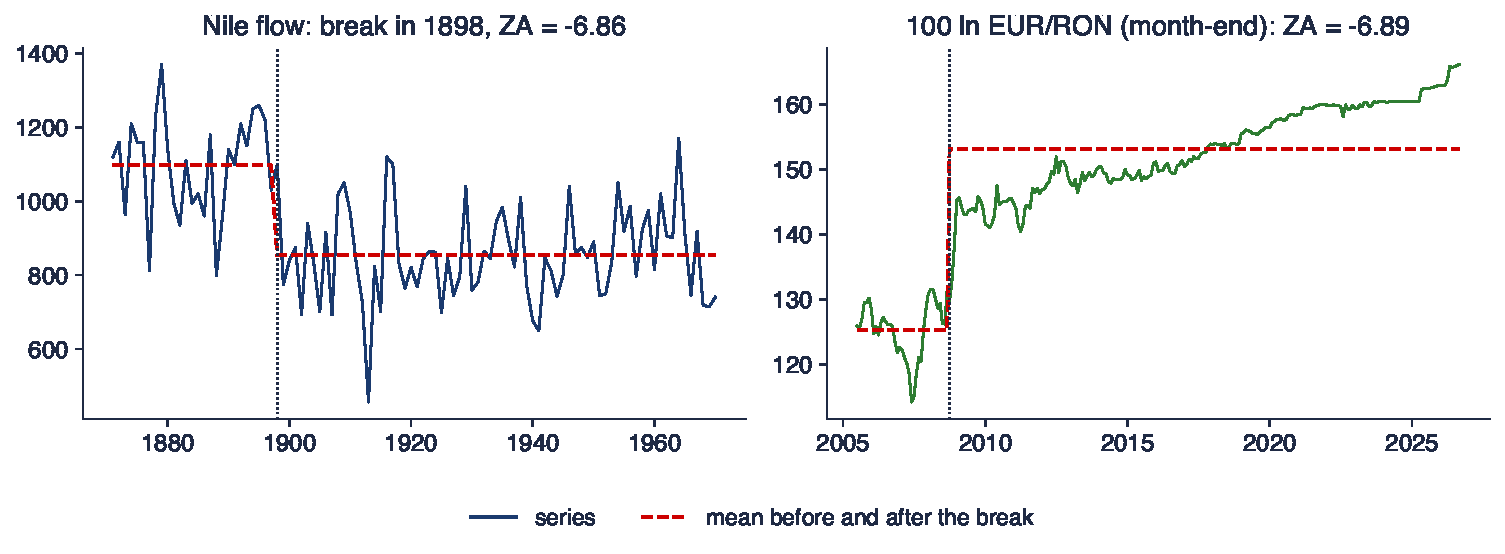
\includegraphics[width=0.97\textwidth,height=0.54\textheight,keepaspectratio]{tsa_ch3_breaks_real.pdf}
\end{center}
\vspace{-0.25cm}
\begin{itemize}
    \item Stînga: debitul Nilului (setul de date statsmodels, 1871--1970); dreapta: 100 ln EUR/RON, cursul de referință BNR de la sfîrșitul lunii
    \item Linia punctată: data rupturii aleasă de test (ruptură în nivel)
\end{itemize}
\quantlet{TSA\_ch3\_structural\_breaks}{\qlurl{TSA_ch3_structural_breaks}}
\end{frame}

\begin{frame}{Interpretarea celor două rupturi}
\itemsize{\small}
\begin{itemize}
    \item Nilul: ZA = $\ensuremath{-}6{,}86$, ruptură în 1898, media scade de la 1098 la 853
    \begin{itemize}
        \item data corespunde istoriei: primul baraj de la Aswan (construit în 1898--1902) și un climat mai secetos; conflictul ADF--KPSS este explicat
    \end{itemize}
    \item EUR/RON (sfîrșit de lună): ADF p = 0{,}55, dar ZA = $\ensuremath{-}6{,}89$, ruptură în octombrie 2008: deprecierea din 2008 (media 3{,}50 lei înainte, 4{,}62 după)
    \begin{itemize}
        \item un curs în regim de managed float: perioade lungi de stabilitate și ajustări rare, nu un mers aleator pur
        \item dar după 2008 cursul continuă să urce: „staționar în jurul unei rupturi” este și el o simplificare
    \end{itemize}
\end{itemize}
\end{frame}

\begin{frame}{Recapitulare: rupturi structurale}
\itemsize{\small}
\begin{itemize}
    \item O schimbare unică a mediei sau a trendului face ca testele de rădăcină unitară să respingă mai rar
    \item Zivot--Andrews caută data rupturii; valorile lui critice sînt mai negative
    \item Rădăcină unitară sau ruptură: comparăm datele cu evenimente cunoscute
\end{itemize}
\end{frame}


%=============================================================================
\section{Modele ARIMA$(p,d,q)$}
%=============================================================================

\begin{frame}{Modelul ARIMA}
\itemsize{\small}
\begin{itemize}
    \item \textbf{Definiție}: $y_t \sim$ ARIMA$(p,d,q)$ (autoregressive integrated moving average, model autoregresiv integrat cu medie mobilă) dacă $\Delta^d y_t$ este un ARMA$(p,q)$ staționar și inversabil:
    \begin{itemize}
        \item $\phi(L)\,(1 - L)^d\,y_t = c + \theta(L)\,\varepsilon_t$, $\varepsilon_t \sim \mathrm{WN}(0, \sigma^2)$
        \item $p$: ordinul AR; $d$: numărul de diferențieri (rădăcini unitare); $q$: ordinul MA; $\phi(L)$, $\theta(L)$ ca în \tsachlink{https://danpele.github.io/Time-Series-Analysis/RO/Cursuri/capitol2_modele_arma.pdf}{Capitolul 2}
    \end{itemize}
    \item Polinomul AR al nivelurilor este $\phi(z)(1 - z)^d$: $d$ rădăcini exact pe cercul unitate
    \begin{itemize}
        \item „integrat”: $y_t$ este o sumă cumulată de $d$ ori a unui proces ARMA
    \end{itemize}
    \item \refBJ\ au popularizat modelul; în practică $d \le 2$, cel mai des $d = 1$
\end{itemize}
\end{frame}

\begin{frame}{Cazuri particulare și constanta}
\itemsize{\small}
\begin{center}
\scriptsize
\begin{tabular}{ll}
\toprule
\textbf{Model} & \textbf{Ecuația și semnificația} \\
\midrule
ARIMA(0,1,0) & $\Delta y_t = c + \varepsilon_t$: mers aleator (cu deriva $c$) \\
ARIMA(1,1,0) & $\Delta y_t = c + \phi\Delta y_{t-1} + \varepsilon_t$: creștere cu inerție \\
ARIMA(0,1,1) & $\Delta y_t = \varepsilon_t + \theta\varepsilon_{t-1}$: netezirea exponențială simplă cu $\alpha = 1 + \theta$ (\tsachlink{https://danpele.github.io/Time-Series-Analysis/RO/Cursuri/capitol0_introducere.pdf}{Capitolul 0}) \\
ARIMA(0,2,2) & $\Delta^2 y_t = \varepsilon_t + \theta_1\varepsilon_{t-1} + \theta_2\varepsilon_{t-2}$: modelul din spatele metodei liniare Holt \\
\bottomrule
\end{tabular}
\end{center}
\begin{itemize}
    \item Constanta $c$ schimbă prognoza pe termen lung \refFPP, cap.~9.7
    \begin{itemize}
        \item $d = 0$: prognozele tind spre medie; $d = 1$: $c \ne 0$ dă o dreaptă (derivă), $c = 0$ o linie orizontală
        \item $d = 2$: $c \ne 0$ dă un trend pătratic, rareori rezonabil; folosim $c = 0$
    \end{itemize}
\end{itemize}
\end{frame}

\begin{frame}{Ciclul Box--Jenkins cu rădăcini unitare}
\itemsize{\small}
\begin{itemize}
    \item \textbf{1. Transformarea}: logaritm sau Box--Cox dacă varianța crește cu nivelul (\tsachlink{https://danpele.github.io/Time-Series-Analysis/RO/Cursuri/capitol1_procese_stochastice_stationaritate.pdf}{Capitolul 1})
    \item \textbf{2. Alegem $d$}: grafic, ACF, ADF și KPSS; testăm întîi $\Delta y_t$; ne oprim la prima diferență staționară
    \item \textbf{3. Alegem $p$, $q$}: ACF și PACF ale lui $\Delta^d y_t$ (\tsachlink{https://danpele.github.io/Time-Series-Analysis/RO/Cursuri/capitol2_modele_arma.pdf}{Capitolul 2}), apoi comparăm candidații după AICc, cu același $d$
    \item \textbf{4. Estimăm} prin verosimilitate maximă; decidem asupra constantei
    \item \textbf{5. Verificăm} reziduurile: ACF, Ljung--Box cu $m - p - q$ grade de libertate, valori extreme
    \item \textbf{6. Prognozăm} nivelurile cu intervale; revenim la pasul 2 sau 3 dacă verificările eșuează
\end{itemize}
\end{frame}

\begin{frame}{PIB-ul României: identificarea}
\itemsize{\footnotesize}
\begin{center}
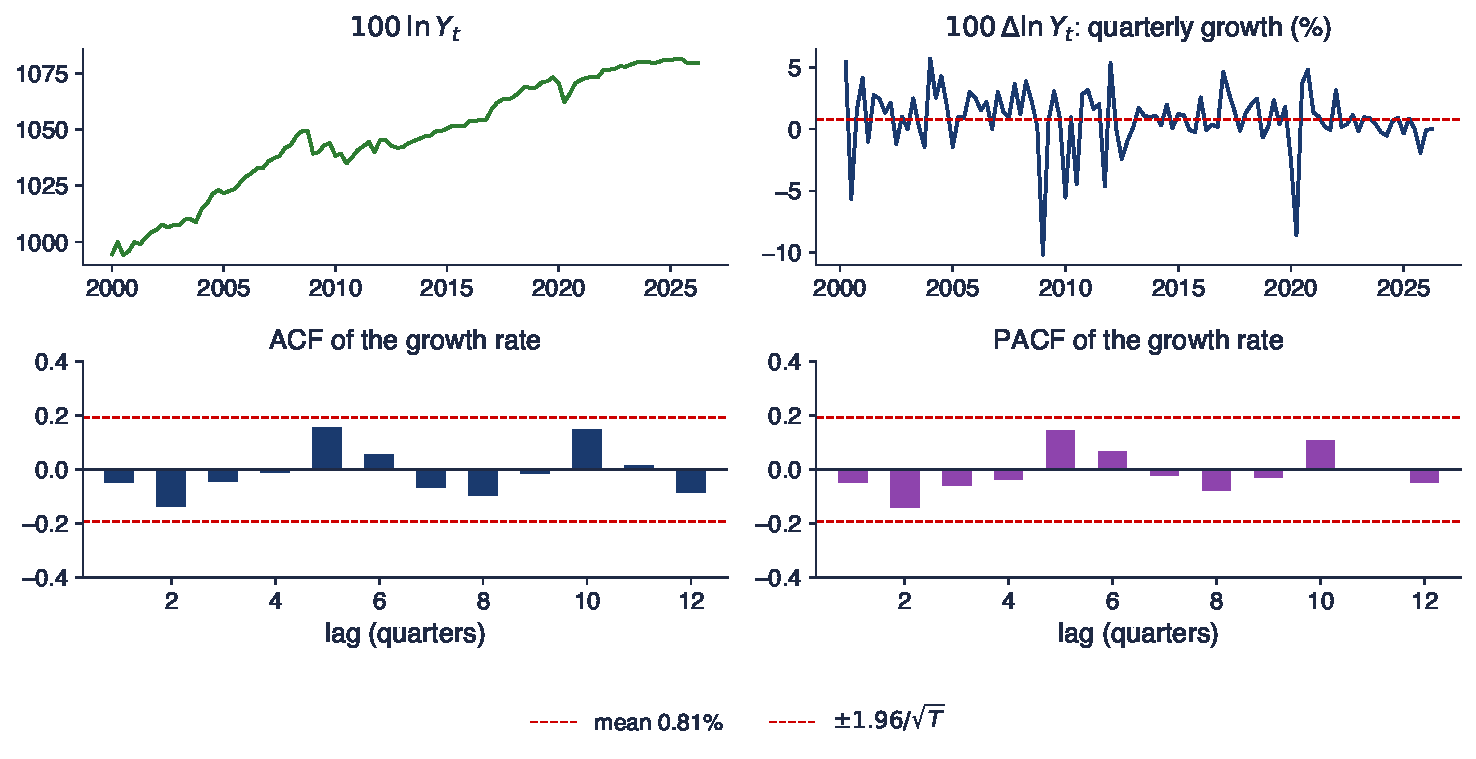
\includegraphics[width=0.97\textwidth,height=0.66\textheight,keepaspectratio]{tsa_ch3_gdp_ident.pdf}
\end{center}
\vspace{-0.25cm}
\begin{itemize}
    \item PIB-ul real ajustat sezonier (Eurostat), T1 2000--T2 2026, $T = 106$; sus: $100\ln Y_t$ și creșterea trimestrială; jos: ACF și PACF ale creșterii
\end{itemize}
\quantlet{TSA\_ch3\_arima\_gdp}{\qlurl{TSA_ch3_arima_gdp}}
\end{frame}

\begin{frame}{Interpretarea graficelor de identificare}
\itemsize{\small}
\begin{itemize}
    \item $d = 1$: nivelul este $I(1)$ (secțiunea 4); rata de creștere este staționară, cu media 0{,}81\% pe trimestru (circa 3{,}2\% pe an)
    \begin{itemize}
        \item două scăderi mari: \ensuremath{-}10{,}2\% în T1 2009 (criza financiară globală) și \ensuremath{-}8{,}6\% în T2 2020 (pandemia)
    \end{itemize}
    \item $p$ și $q$: nicio valoare ACF sau PACF în afara benzii $\pm 0{,}19$; $\hat\rho(1) = \ensuremath{-}0{,}05$, $\hat\rho(2) = \ensuremath{-}0{,}14$
    \begin{itemize}
        \item Ljung--Box $Q^*(8) = 7{,}3$ (p = 0{,}51): rata de creștere seamănă cu un zgomot alb în jurul mediei
    \end{itemize}
    \item Graficele sugerează ARIMA(0,1,0) cu derivă; slide-ul următor verifică alternativele
\end{itemize}
\end{frame}

\begin{frame}{Alegerea modelului după AICc}
\itemsize{\small}
\begin{center}
\footnotesize
\begin{tabular}{lccc}
\toprule
& $q = 0$ & $q = 1$ & $q = 2$ \\
\midrule
$p = 0$ & 491{,}9 & 493{,}7 & 493{,}6 \\
$p = 1$ & 493{,}8 & 494{,}9 & 495{,}8 \\
$p = 2$ & 493{,}7 & 495{,}7 & 495{,}4$^\dagger$ \\
\bottomrule
\end{tabular}
\end{center}
\begin{itemize}
    \item ARIMA$(p,1,q)$ cu derivă pentru $100\ln Y_t$, estimat prin verosimilitate maximă; AICc: AIC cu corecția pentru eșantioane mici (\tsachlink{https://danpele.github.io/Time-Series-Analysis/RO/Cursuri/capitol2_modele_arma.pdf}{Capitolul 2}); $^\dagger$: optimizarea nu a convers
    \item Cel mai mic AICc: ARIMA(0,1,0); următorul model este cu 1{,}7 puncte mai slab
    \begin{itemize}
        \item diferențele sub 2 puncte nu sînt relevante: păstrăm cel mai simplu model
    \end{itemize}
    \item Estimarea: deriva $\hat c = 0{,}81$ (SE 0{,}30, $t = 2{,}72$), $\hat\sigma = 2{,}47$: $100\,\Delta\ln Y_t = 0{,}81 + \hat\varepsilon_t$
\end{itemize}\quantlet{TSA\_ch3\_arima\_gdp}{\qlurl{TSA_ch3_arima_gdp}}
\end{frame}

\begin{frame}{PIB-ul României: verificarea reziduurilor}
\itemsize{\footnotesize}
\begin{center}
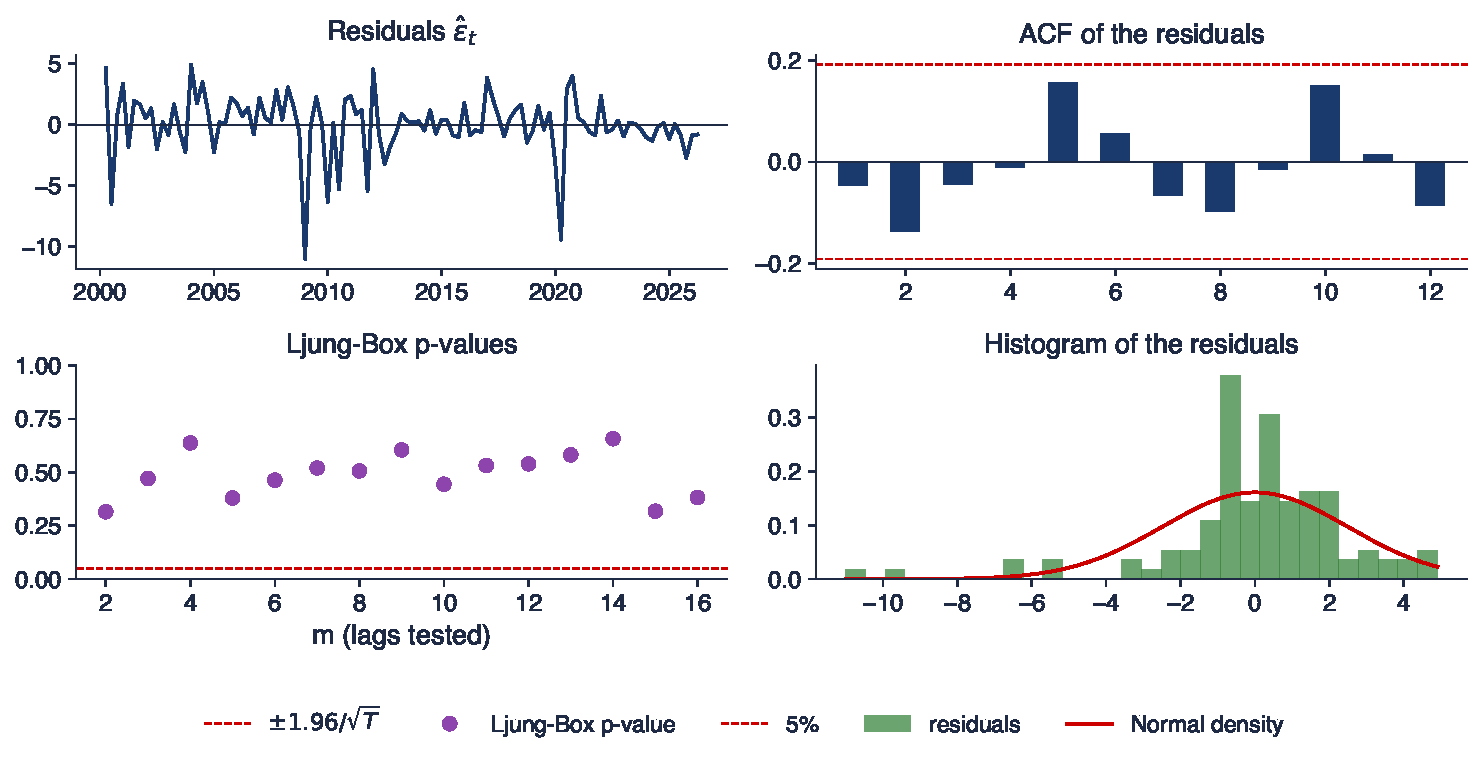
\includegraphics[width=0.97\textwidth,height=0.66\textheight,keepaspectratio]{tsa_ch3_gdp_diag.pdf}
\end{center}
\vspace{-0.25cm}
\begin{itemize}
    \item Reziduurile modelului ARIMA(0,1,0) cu derivă: graficul în timp, ACF, p-value-urile Ljung--Box pentru $m = 2, \dots, 16$, histograma cu densitatea Normală
\end{itemize}
\quantlet{TSA\_ch3\_arima\_gdp}{\qlurl{TSA_ch3_arima_gdp}}
\end{frame}

\begin{frame}{Interpretarea verificării reziduurilor}
\itemsize{\small}
\begin{itemize}
    \item Nu a rămas autocorelație: $Q^*(8) = 7{,}3$ (p = 0{,}51), $Q^*(12)$ p = 0{,}54; toate p-value-urile sînt peste 5\%
    \item Nu sînt normale: kurtosis-ul 7{,}9, Jarque--Bera 145; cel mai mare reziduu este $\ensuremath{-}11{,}0$ în T1 2009
    \begin{itemize}
        \item două crize domină cozile; intervalele normale din slide-urile următoare sînt prea înguste într-o criză și ușor prea largi în perioadele calme
        \item opțiuni: variabile dummy pentru 2009 și 2020 sau un bootstrap al reziduurilor pentru intervale
    \end{itemize}
\end{itemize}
\end{frame}

\begin{frame}{Prognoza cu modele ARIMA}
\itemsize{\small}
\begin{itemize}
    \item \textbf{Prognozele punctuale}: scriem modelul pentru niveluri și îl aplicăm recursiv, cu $\hat\varepsilon_{T+j} = 0$ pentru $j \ge 1$
    \begin{itemize}
        \item ARIMA(1,1,0): $y_t = (1 + \phi)y_{t-1} - \phi y_{t-2} + \varepsilon_t$
    \end{itemize}
    \item \textbf{Eroarea de prognoză}: $y_{T+h} - \hat y_{T+h} = \sum_{j=0}^{h-1}\psi_j\varepsilon_{T+h-j}$, cu $\psi(z) = \theta(z)/[\phi(z)(1 - z)^d]$
    \begin{itemize}
        \item varianța $\sigma^2\sum_{j=0}^{h-1}\psi_j^2$; intervalul de 95\%: $\hat y_{T+h} \pm 1{,}96\,\sigma\sqrt{\sum_{j<h}\psi_j^2}$
        \item pentru $d \ge 1$, $\psi_j$ nu tind la 0: varianța crește nelimitat
    \end{itemize}
    \item Două formule explicite
    \begin{itemize}
        \item mersul aleator: $\psi_j = 1$, varianța $h\sigma^2$: intervalul crește ca $\sqrt{h}$
        \item ARIMA(0,1,1): $\psi_j = 1 + \theta$ pentru $j \ge 1$, varianța $\sigma^2[1 + (h - 1)(1 + \theta)^2]$
    \end{itemize}
\end{itemize}
\end{frame}

\begin{frame}{Exemplu rezolvat: prognoze ARIMA(1,1,0)}
\itemsize{\small}
\begin{itemize}
    \item $\Delta y_t = 0{,}6\,\Delta y_{t-1} + \varepsilon_t$, $\sigma = 2$; ultimele date: $y_T = 108$, $\Delta y_T = 5$
    \item \textbf{Prognozele punctuale}: prognozăm variația, apoi o adunăm
    \begin{itemize}
        \item $\widehat{\Delta y}_{T+1} = 0{,}6 \cdot 5 = 3$, $\hat y_{T+1} = 111{,}00$; $\widehat{\Delta y}_{T+2} = 1{,}8$, $\hat y_{T+2} = 112{,}80$; $\hat y_{T+3} = 113{,}88$
    \end{itemize}
    \item \textbf{Ponderile $\psi$}: $\psi_0 = 1$, $\psi_1 = 1 + \phi = 1{,}60$, $\psi_2 = 1 + \phi + \phi^2 = 1{,}96$
    \begin{itemize}
        \item varianțele: $4$, $4(1 + 1{,}60^2) = 14{,}24$, $4(1 + 1{,}60^2 + 1{,}96^2) = 29{,}61$
        \item semilățimile de 95\%: 3{,}92; 7{,}40; 10{,}66: intervalul aproape se triplează în trei pași
    \end{itemize}
    \item Inerția $\phi = 0{,}6$ face ca incertitudinea să crească mai repede decît la un mers aleator ($\sqrt{3} = 1{,}73$ ori în trei pași)
\end{itemize}
\end{frame}

\begin{frame}{Viteza de creștere a intervalelor}
\itemsize{\footnotesize}
\begin{center}
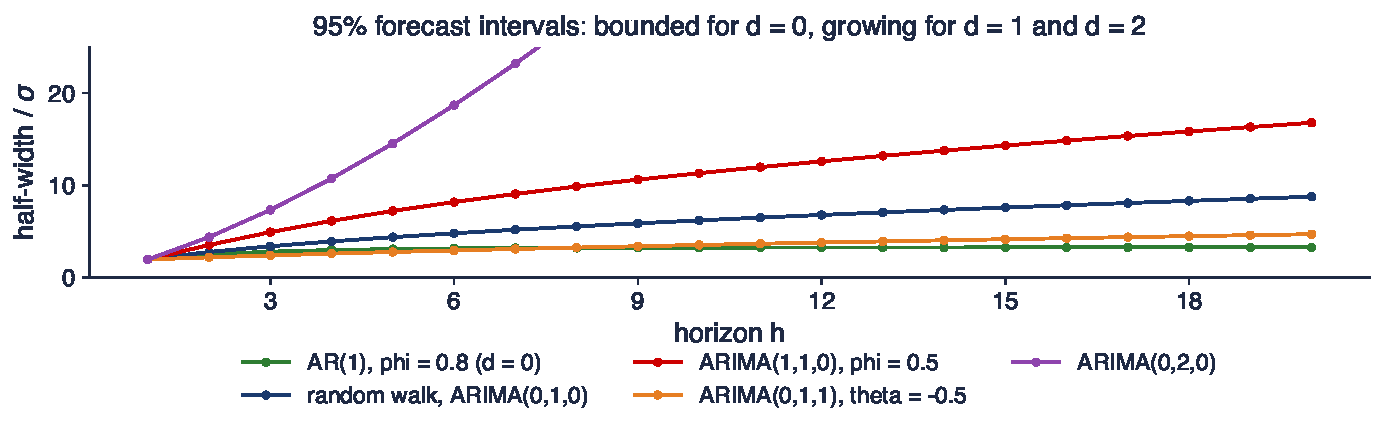
\includegraphics[width=0.97\textwidth,height=0.56\textheight,keepaspectratio]{tsa_ch3_interval_width.pdf}
\end{center}
\vspace{-0.25cm}
\begin{itemize}
    \item Semilățimea intervalului de prognoză de 95\%, în unități $\sigma$, pentru orizonturile 1--20, din ponderile $\psi$ ale a cinci modele
\end{itemize}
\quantlet{TSA\_ch3\_forecast\_intervals}{\qlurl{TSA_ch3_forecast_intervals}}
\end{frame}

\begin{frame}{Interpretarea lățimii intervalelor}
\itemsize{\small}
\begin{itemize}
    \item $d = 0$, AR(1) cu $\phi = 0{,}8$: lățimea se stabilizează la $1{,}96\sigma/\sqrt{1 - \phi^2}$ (3{,}27$\sigma$ la $h = 20$)
    \item $d = 1$: creștere ca $\sqrt{h}$; la $h = 20$: 8{,}77$\sigma$ (mers aleator), 16{,}78$\sigma$ (ARIMA(1,1,0)), 4{,}70$\sigma$ (ARIMA(0,1,1), $\theta = -0{,}5$)
    \begin{itemize}
        \item o componentă MA negativă compensează o parte din fiecare șoc: intervale mai înguste
    \end{itemize}
    \item $d = 2$: creștere ca $h^{3/2}$ (105{,}00$\sigma$ la $h = 20$): supradiferențierea face prognozele pe termen lung inutilizabile
\end{itemize}
\end{frame}

\begin{frame}{PIB-ul României: două prognoze}
\itemsize{\footnotesize}
\begin{center}
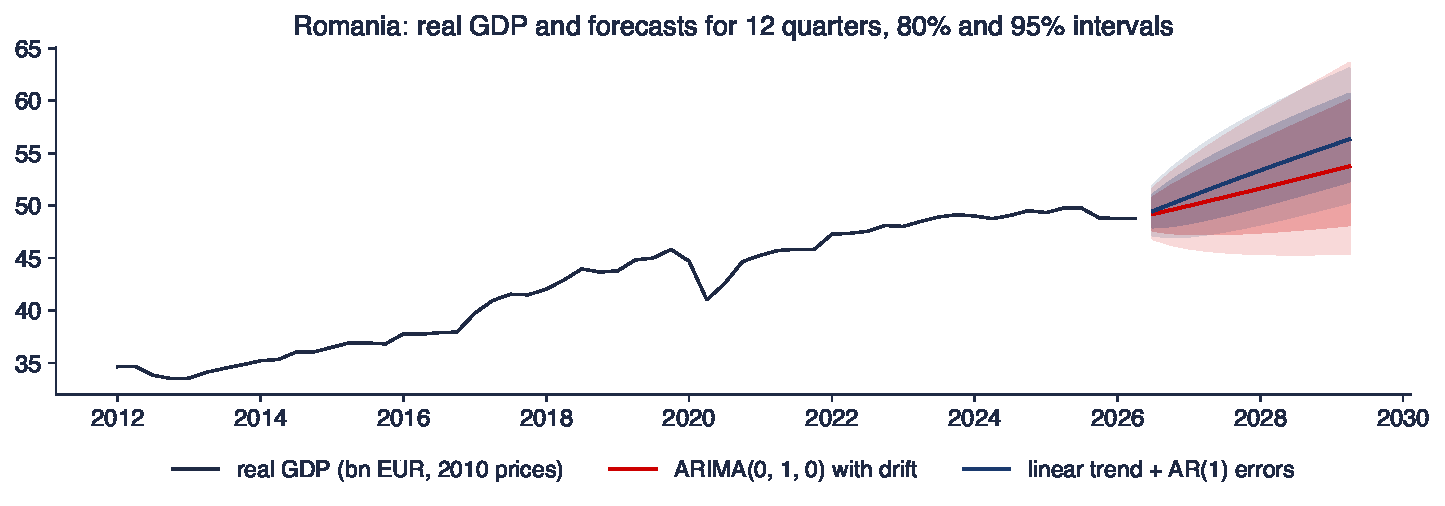
\includegraphics[width=0.97\textwidth,height=0.56\textheight,keepaspectratio]{tsa_ch3_gdp_forecast.pdf}
\end{center}
\vspace{-0.25cm}
\begin{itemize}
    \item ARIMA(0,1,0) cu derivă (roșu) și un trend liniar cu erori AR(1) (albastru), ambele estimate pe T1 2000--T2 2026; prognoze pînă în T2 2029, transformate înapoi în mld. EUR
\end{itemize}
\quantlet{TSA\_ch3\_arima\_gdp}{\qlurl{TSA_ch3_arima_gdp}}
\end{frame}

\begin{frame}{Interpretarea prognozelor PIB}
\itemsize{\small}
\begin{itemize}
    \item Mersul aleator cu derivă crește cu 0{,}81\% pe trimestru de la ultima valoare (48{,}8 mld. EUR în T2 2026): 53{,}8 mld. după 12 trimestre
    \begin{itemize}
        \item semilățimea de 95\% (în \% din PIB): 4{,}8 după 1 trimestru, 9{,}7 după 4, 16{,}8 după 12, adică $\times$3{,}46 $= \sqrt{12}$
    \end{itemize}
    \item Modelul staționar în jurul trendului readuce PIB-ul spre vechea dreaptă ($\hat\phi = 0{,}92$): 56{,}3 mld. după 12 trimestre, semilățimea 11{,}2\%
    \begin{itemize}
        \item mai optimist și cu intervale mai înguste, pentru că presupune că încetinirea recentă este temporară
    \end{itemize}
    \item Testele nu au putut decide între cele două modele pe acest eșantion: alegerea lui $d$ este o decizie de prognoză cu consecințe
\end{itemize}
\end{frame}

\begin{frame}{Supradiferențierea}
\itemsize{\small}
\begin{itemize}
    \item Diferențierea unei serii $I(0)$ creează o rădăcină unitară MA: $\Delta\varepsilon_t = \varepsilon_t - \varepsilon_{t-1}$, $\theta = -1$ (\tsachlink{https://danpele.github.io/Time-Series-Analysis/RO/Cursuri/capitol1_procese_stochastice_stationaritate.pdf}{Capitolul 1})
    \begin{itemize}
        \item rezultatul nu este inversabil: nu are reprezentare AR($\infty$), iar estimarea este dificilă \refPS
    \end{itemize}
    \item Simptome
    \begin{itemize}
        \item $\hat\rho(1)$ al seriei diferențiate apropiat de $-0{,}5$
        \item varianța crește după diferențiere, în loc să scadă
        \item un coeficient MA estimat apropiat de $-1$
    \end{itemize}
    \item Regula: diferențiem doar cît timp varianța scade și testele o cer
\end{itemize}
\end{frame}

\begin{frame}{Supradiferențierea PIB-ului României}
\itemsize{\footnotesize}
\begin{center}
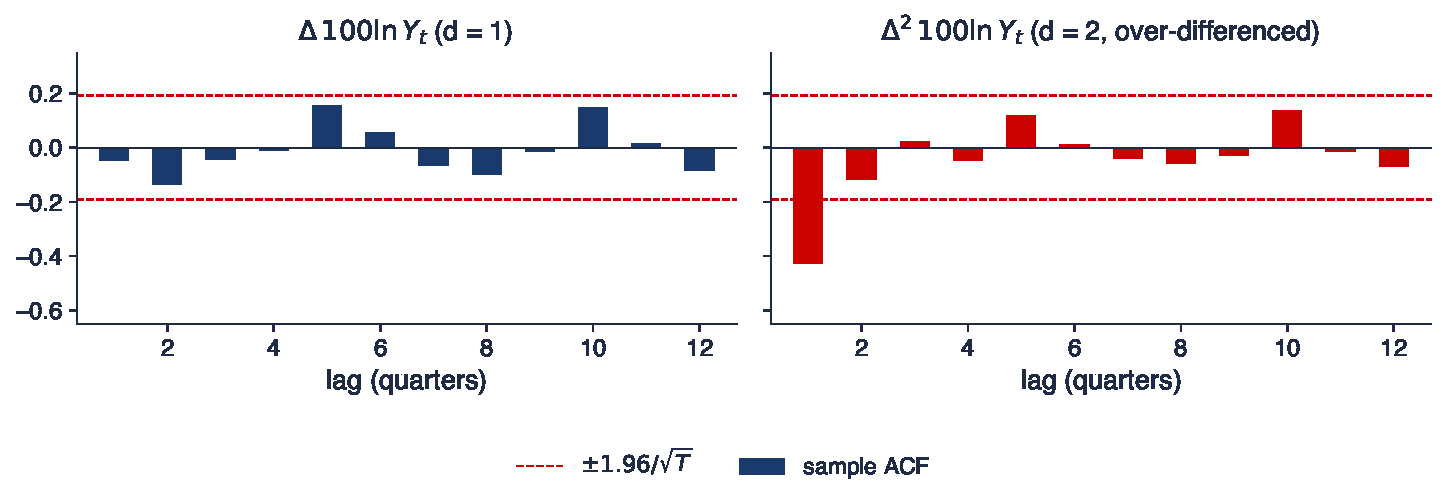
\includegraphics[width=0.97\textwidth,height=0.48\textheight,keepaspectratio]{tsa_ch3_overdiff_gdp.pdf}
\end{center}
\vspace{-0.25cm}
\begin{itemize}
    \item ACF a creșterii trimestriale $\Delta\,100\ln Y_t$ ($d = 1$) și a diferenței ei $\Delta^2\,100\ln Y_t$ ($d = 2$)
\end{itemize}
\quantlet{TSA\_ch3\_arima\_gdp}{\qlurl{TSA_ch3_arima_gdp}}
\end{frame}

\begin{frame}{Interpretarea supradiferențierii}
\itemsize{\small}
\begin{itemize}
    \item $d = 1$: $\hat\rho(1) = \ensuremath{-}0{,}05$, varianța 6{,}16; $d = 2$: $\hat\rho(1) = \ensuremath{-}0{,}43$, varianța 12{,}80: toate cele trei simptome
    \item Un MA(1) estimat pe $\Delta^2\,100\ln Y_t$ dă $\hat\theta = \ensuremath{-}0{,}987$ (SE 0{,}080): practic $-1$, diferența în plus este anulată de partea MA
    \item Alegerea corectă: $d = 1$
\end{itemize}
\end{frame}

\begin{frame}{Recapitulare: modele ARIMA}
\itemsize{\small}
\begin{itemize}
    \item ARIMA$(p,d,q)$: un ARMA$(p,q)$ pentru $\Delta^d y_t$; constanta decide panta pe termen lung
    \item PIB-ul României din 2000: ARIMA(0,1,0) cu derivă, 0{,}81\% pe trimestru; reziduuri necorelate, dar cu cozi groase
    \item Varianța prognozei $\sigma^2\sum_{j<h}\psi_j^2$: mărginită pentru $d = 0$, crescătoare pentru $d \ge 1$
    \item Supradiferențierea: $\hat\rho(1) \approx -0{,}5$, varianță mai mare, coeficient MA apropiat de $-1$
\end{itemize}
\end{frame}


%=============================================================================
\section{ARIMA în practică}
%=============================================================================

\begin{frame}{Selecția automată ARIMA}
\itemsize{\small}
\begin{itemize}
    \item \refHK\ (\texttt{auto.arima} în R; \texttt{pmdarima} și \texttt{statsforecast} în Python):
    \begin{itemize}
        \item $d$: teste KPSS repetate la 5\%: diferențiem cît timp KPSS respinge
        \item $p$, $q$: o căutare pas cu pas pornind de la cîteva modele inițiale, după AICc, cu $d$ ales; constantă sau derivă dacă $d \le 1$
        \item elimină modelele cu rădăcini prea apropiate de cercul unitate și estimările care eșuează
    \end{itemize}
    \item Util pentru multe serii deodată și ca punct de plecare
    \begin{itemize}
        \item evaluată de autori pe cele 3\,003 serii ale competiției de prognoză M3, metoda a fost competitivă cu cele mai bune metode din competiție
    \end{itemize}
    \item Dar fiecare pas conține o alegere pe care trebuie să o puteți justifica (slide-ul următor)
\end{itemize}
\end{frame}

\begin{frame}{Selecția automată ARIMA: verificări}
\itemsize{\small}
\begin{itemize}
    \item \textbf{AICc nu este comparabil între valori diferite ale lui $d$}: cu $d = 1$, verosimilitatea se calculează pentru $\Delta y_t$, o altă serie
    \begin{itemize}
        \item alegem $d$ prin teste și judecată, apoi comparăm $p$ și $q$
    \end{itemize}
    \item \textbf{Rădăcini care aproape se anulează}: PIB-ul României din T1 1995: cel mai mic AICc, 607{,}5 (ARIMA(0,1,0): 611{,}1), aparține modelului ARIMA(2,1,2), a cărui estimare nu a convers
    \begin{itemize}
        \item rădăcini MA de modul 1{,}0002, rădăcini AR 1{,}014: AR și MA aproape se anulează; $\hat\theta_2 = 1{,}000$ cu SE 6{,}96
        \item un model ajustat pe zgomotul datelor din anii 1990, nu o descriere a economiei
    \end{itemize}
    \item \textbf{Întotdeauna}: reprezentăm grafic datele, verificăm convergența și rădăcinile, aplicăm testele pe reziduuri, comparăm cu o metodă simplă de referință (mersul aleator, \tsachlink{https://danpele.github.io/Time-Series-Analysis/RO/Cursuri/capitol0_introducere.pdf}{Capitolul 0})
\end{itemize}
\end{frame}

\begin{frame}{Inflația din România: $d = 0$ sau $d = 1$?}
\itemsize{\footnotesize}
\begin{center}
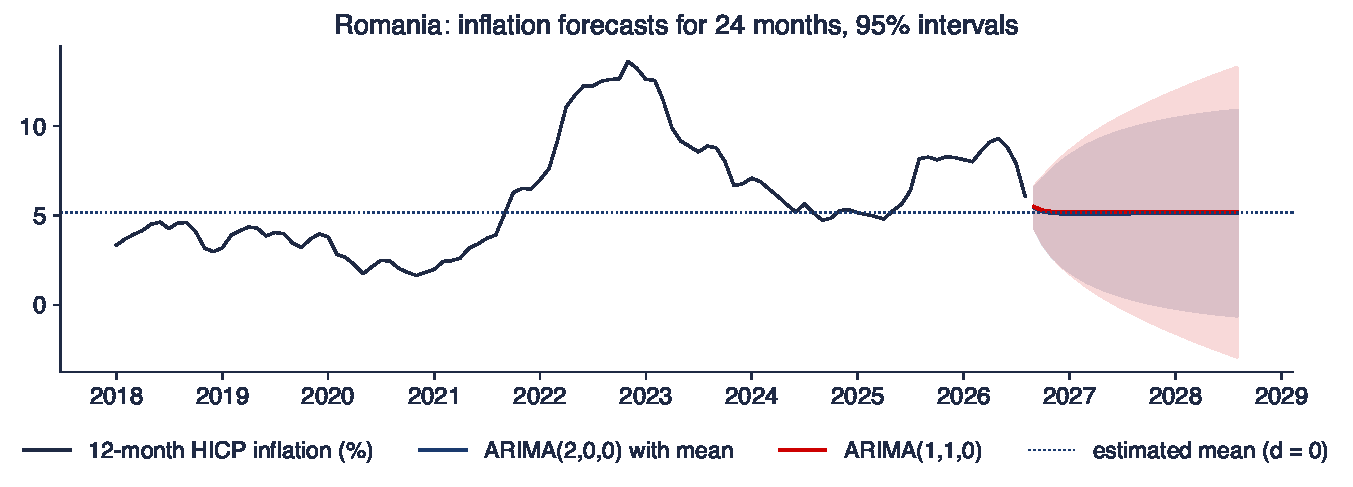
\includegraphics[width=0.97\textwidth,height=0.54\textheight,keepaspectratio]{tsa_ch3_inflation_d.pdf}
\end{center}
\vspace{-0.25cm}
\begin{itemize}
    \item Inflația anuală IAPC (Eurostat), ianuarie 2005--august 2026; cel mai bun model după AICc pentru $d = 0$ (cu medie) și pentru $d = 1$, $p \le 3$, $q \le 2$; prognoze pentru 24 de luni
\end{itemize}
\quantlet{TSA\_ch3\_arima\_in\_practice}{\qlurl{TSA_ch3_arima_in_practice}}
\end{frame}

\begin{frame}{Interpretarea celor două modele ale inflației}
\itemsize{\small}
\begin{itemize}
    \item $d = 0$: ARIMA(2,0,0), $\hat\phi_1 = 1{,}32$, $\hat\phi_2 = \ensuremath{-}0{,}34$, suma 0{,}976: staționar, dar la limită; media 5{,}2\%
    \begin{itemize}
        \item $d = 1$: ARIMA(1,1,0), $\hat\phi = 0{,}33$: aproape aceeași dinamică pe termen scurt
    \end{itemize}
    \item După 24 de luni: 5{,}1\% în $[\ensuremath{-}0{,}6; 10{,}9]$, față de 5{,}2\% în $[\ensuremath{-}2{,}9; 13{,}3]$
    \begin{itemize}
        \item prognoze punctuale similare, intervale diferite: $d$ decide cîtă incertitudine raportăm
    \end{itemize}
    \item KPSS (0{,}404) păstrează $d = 0$, ca selecția automată; ADF (p = 0{,}32) sugerează $d = 1$
    \begin{itemize}
        \item ambele modele lasă reziduuri autocorelate: ratele anuale se suprapun și moștenesc sezonalitatea; \tsachlink{https://danpele.github.io/Time-Series-Analysis/RO/Cursuri/capitol4_sezonalitate_prognoza.pdf}{Capitolul 4} modelează inflația lunară
    \end{itemize}
\end{itemize}
\end{frame}

\begin{frame}{Studiu de caz: Meese și Rogoff (1983)}
\itemsize{\small}
\begin{itemize}
    \item \textbf{Întrebarea}: pot modelele cursului de schimb să prognozeze mai bine decît un mers aleator?
    \begin{itemize}
        \item \refMR: modelele monetare din anii 1970, modele de serii de timp (ARIMA, VAR) și mersul aleator; cursuri ale dolarului, orizonturi de 1--12 luni
    \end{itemize}
    \item \textbf{Rezultatul}: în afara eșantionului, niciun model nu a depășit mersul aleator ca RMSE (root mean squared error, rădăcina erorii pătratice medii)
    \begin{itemize}
        \item nici măcar atunci cînd au folosit valorile viitoare efective ale variabilelor fundamentale
    \end{itemize}
    \item \textbf{Moștenirea}: „enigma Meese--Rogoff” și mersul aleator ca reper pentru orice prognoză a cursului de schimb
    \begin{itemize}
        \item graficul următor: aceeași comparație pentru EUR/RON
    \end{itemize}
\end{itemize}
\end{frame}

\begin{frame}{EUR/RON: ARIMA față de mersul aleator}
\itemsize{\footnotesize}
\begin{center}
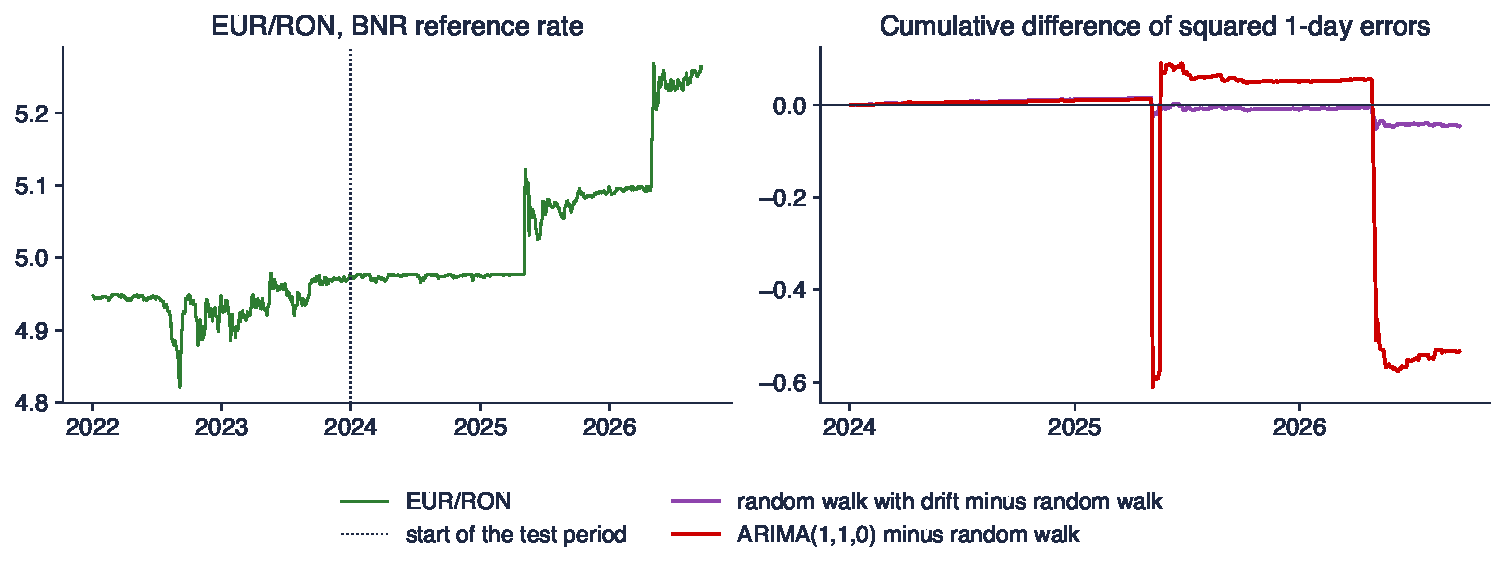
\includegraphics[width=0.97\textwidth,height=0.52\textheight,keepaspectratio]{tsa_ch3_eurron_forecast.pdf}
\end{center}
\vspace{-0.25cm}
\begin{itemize}
    \item Parametrii estimați pe 4\,673 de variații zilnice pînă în decembrie 2023; 679 de prognoze cu o zi înainte din ianuarie 2024; dreapta: diferența cumulată a erorilor pătratice (sub 0: modelul este mai precis decît mersul aleator)
\end{itemize}
\quantlet{TSA\_ch3\_arima\_in\_practice}{\qlurl{TSA_ch3_arima_in_practice}}
\end{frame}

\begin{frame}{Interpretarea comparației EUR/RON}
\itemsize{\small}
\begin{itemize}
    \item RMSE al variației zilnice ($100\ln$): mers aleator 0{,}1330, cu derivă 0{,}1327, ARIMA(1,1,0) 0{,}1300 ($\hat\phi = 0{,}169$)
    \begin{itemize}
        \item un cîștig de 2{,}2\%; pe 20 de zile (33 de ferestre fără suprapunere): 0{,}667 față de 0{,}638, un cîștig de 4{,}3\%
    \end{itemize}
    \item Cîștigul provine din cîteva zile: două salturi ale cursului (de la 4{,}9746 la 5{,}2644 lei în perioada analizată) au continuat și a doua zi
    \begin{itemize}
        \item în zilele calme, mersul aleator este la fel de bun; o comparație formală cere testul Diebold--Mariano (\tsachlink{https://danpele.github.io/Time-Series-Analysis/RO/Cursuri/capitol4_sezonalitate_prognoza.pdf}{Capitolul 4})
    \end{itemize}
    \item Lecția Meese--Rogoff: raportăm mersul aleator alături de orice prognoză a cursului de schimb
\end{itemize}
\end{frame}

\begin{frame}{O serie clasică: PIB-ul real al SUA după 2007}
\itemsize{\footnotesize}
\begin{center}
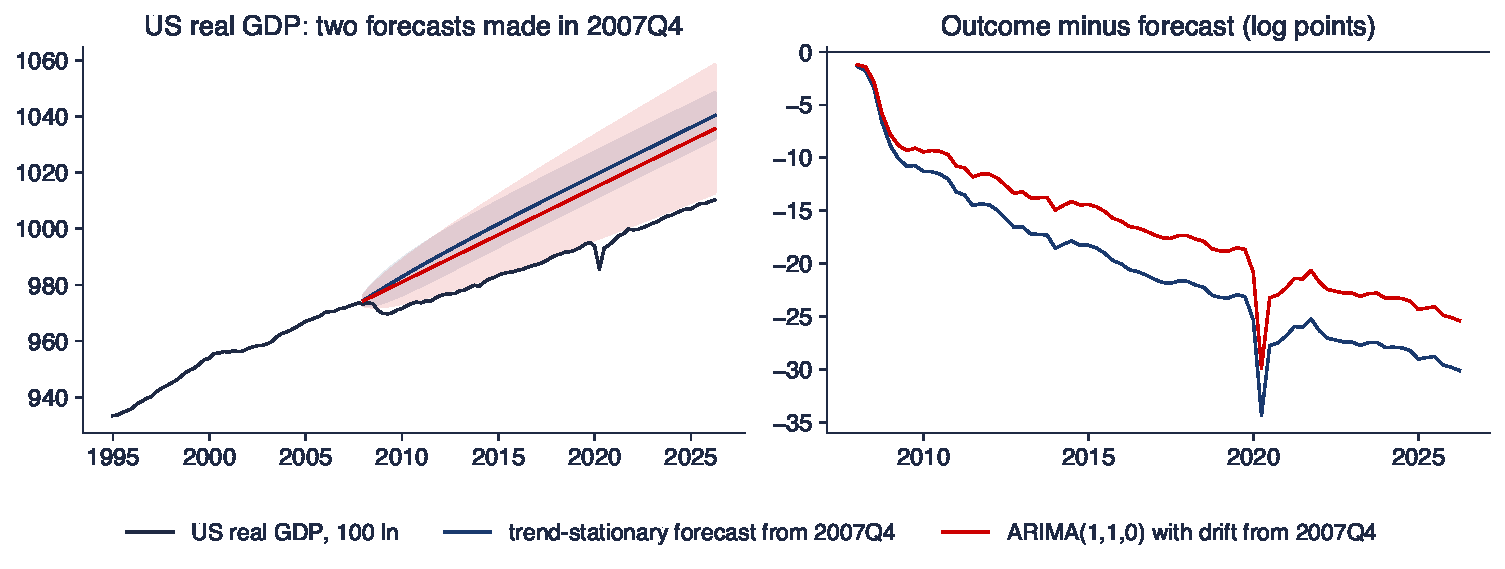
\includegraphics[width=0.97\textwidth,height=0.54\textheight,keepaspectratio]{tsa_ch3_us_gdp.pdf}
\end{center}
\vspace{-0.25cm}
\begin{itemize}
    \item Seria FRED GDPC1 din 1947; un model staționar în jurul trendului (trend liniar, erori AR(2)) și unul staționar în diferențe (ARIMA(1,1,0) cu derivă), estimate pînă în T4 2007 și prognozate pînă în T2 2026; intervale de 95\%
\end{itemize}
\quantlet{TSA\_ch3\_us\_gdp}{\qlurl{TSA_ch3_us_gdp}}
\end{frame}

\begin{frame}{Interpretarea prognozelor PIB-ului SUA}
\itemsize{\small}
\begin{itemize}
    \item Modelul staționar în jurul trendului aștepta o revenire la dreapta de dinainte de 2008; abaterea s-a mărit continuu: $\ensuremath{-}30$ puncte logaritmice la final (semilățimea intervalului: 8)
    \begin{itemize}
        \item pierderea din 2008--2009 nu a fost recuperată niciodată: o dovadă a unui șoc permanent, cum implică viziunea \refNP
    \end{itemize}
    \item Și modelul staționar în diferențe greșește ($\ensuremath{-}25$), dar intervalul lui (semilățimea 23) avertizează măcar asupra incertitudinii mari
    \begin{itemize}
        \item ambele presupun aceeași derivă ca înainte de 2008; creșterea de după 2008 a fost mai lentă: o ruptură în derivă (secțiunea 5)
    \end{itemize}
    \item Testele de rădăcină unitară pe întreaga serie: ADF p = 0{,}82, KPSS 0{,}58: $I(1)$
\end{itemize}
\end{frame}

\begin{frame}{Recapitulare: ARIMA în practică}
\itemsize{\small}
\begin{itemize}
    \item Selecția automată ARIMA: KPSS pentru $d$, AICc pentru $p$ și $q$; verificăm convergența, rădăcinile și reziduurile
    \item AICc compară doar modele cu același $d$
    \item Cursurile de schimb: mersul aleator este un reper greu de depășit \refMR
    \item Alegerea între staționaritate în jurul trendului și în diferențe schimbă prognoza pe termen lung și intervalul ei: PIB-ul SUA după 2008
\end{itemize}
\end{frame}


%=============================================================================
\section{Contribuția posibilă a AI}
%=============================================================================

\begin{frame}{Contribuția posibilă a AI}
\itemsize{\small}
\begin{itemize}
    \item \textbf{Cod}: o primă versiune a unui script care aplică ADF, PP și KPSS pe multe serii și tabelează verdictele
    \item \textbf{Explicații}: o a doua explicație a motivului pentru care distribuția Dickey--Fuller nu este Normală sau a unui rezultat ZA
    \item \textbf{Explorare}: rădăcini unitare și rupturi în toate ratele inflației din UE sau modele ARIMA de referință pentru multe serii românești
    \item Exemplu de prompt
    \begin{itemize}
        \item \aiprompt{Write Python code that loads Romanian quarterly real GDP (Eurostat namq\_10\_gdp, seasonally adjusted), runs ADF with constant and trend and KPSS on 100*log GDP and on its difference, fits ARIMA(p,1,q) with drift for p, q <= 2, and plots 8-quarter forecasts with 95\% intervals.}
    \end{itemize}
\end{itemize}
\end{frame}

\begin{frame}{Verificări necesare}
\itemsize{\small}
\begin{itemize}
    \item Sensul fiecărui test: ADF și PP au rădăcina unitară ca $H_0$, KPSS are staționaritatea ca $H_0$
    \item Termenii determiniști, numărul de laguri și valorile critice folosite efectiv (Dickey--Fuller, nu ale distribuției Normale)
    \item Că „nerespins” nu este raportat ca „demonstrat”
    \item Că regresiile între serii cu trend nu sînt prezentate drept dovezi de cauzalitate
    \item Avertismentele de convergență, rădăcinile apropiate de cercul unitate, testele pe reziduuri și compararea AICc doar pentru același $d$
    \item Fiecare referință citată: trebuie să existe; verificați DOI-ul
\end{itemize}
\end{frame}


%=============================================================================
\section{Rezumat}
%=============================================================================

\begin{frame}{Idei de reținut}
\itemsize{\small}
\begin{itemize}
    \item Seriile cu trend sînt staționare în jurul trendului (șocurile se sting) sau staționare în diferențe (șocurile sînt permanente); tratamentul diferă: eliminăm trendul sau diferențiem
    \item Regresiile între serii $I(1)$ fără legătură sînt false: $t$ și $R^2$ mari, DW apropiat de 0
    \item ADF și PP testează $H_0$: rădăcină unitară, cu valori critice Dickey--Fuller; KPSS testează $H_0$: staționaritate; le folosim împreună
    \item Testele au putere mică în apropierea lui $\phi = 1$ și sînt înșelate de rupturi; Zivot--Andrews permite o ruptură
    \item ARIMA$(p,d,q)$ = ARMA pe $\Delta^d y_t$; intervalele de prognoză cresc cu orizontul cînd $d \ge 1$
    \item Selecția automată este un punct de plecare: verificăm $d$, convergența, rădăcinile, reziduurile și comparația cu mersul aleator
\end{itemize}
\end{frame}

\begin{frame}{Formule de reținut}
\itemsize{\small}
{\renewcommand{\arraystretch}{1.4}\begin{center}
\scriptsize
\begin{tabular}{ll}
\toprule
\textbf{Mărimea} & \textbf{Formula} \\
\midrule
Cele două tipuri de trend & $y_t = \alpha + \beta t + u_t$, \quad $\Delta y_t = \beta + u_t$, \quad $u_t \sim I(0)$ \\
ADF & $\Delta y_t = c + bt + \gamma y_{t-1} + \sum_{j=1}^{k}\delta_j\Delta y_{t-j} + \varepsilon_t$, \quad $H_0$: $\gamma = 0$, \quad $\tau = \hat\gamma/\mathrm{SE}(\hat\gamma)$ \\
Laguri & $k_{\max} = 12\,(T/100)^{1/4}$, apoi AIC sau BIC \\
KPSS & $\eta = \sum_{t=1}^{T} S_t^2/(T^2\hat\lambda^2)$, \quad $S_t = \sum_{s \le t} e_s$, \quad 5\%: 0,463 (c); 0,146 (c, t) \\
ARIMA$(p,d,q)$ & $\phi(L)(1 - L)^d y_t = c + \theta(L)\varepsilon_t$ \\
Varianța prognozei & $\sigma^2\sum_{j=0}^{h-1}\psi_j^2$, \quad $\psi(z) = \theta(z)/[\phi(z)(1 - z)^d]$; mers aleator: $h\sigma^2$ \\
ARIMA(0,1,1) & $\sigma^2[1 + (h - 1)(1 + \theta)^2]$, \quad $\alpha_{\mathrm{SES}} = 1 + \theta$ \\
\bottomrule
\end{tabular}
\end{center}
}
\end{frame}

\begin{frame}{Autoevaluare}
\itemsize{\small}
\begin{itemize}
    \item \textbf{Întrebare}: un test ADF cu constantă și trend dă $\tau = -2{,}9$ pentru $T = 200$. Respingeți rădăcina unitară la 5\%?
    \begin{itemize}
        \item \textbf{Răspuns}: nu: $-2{,}9 > -3{,}43$; cu tabelul distribuției Normale ați respinge greșit
    \end{itemize}
    \item \textbf{Întrebare}: ADF nu respinge, iar KPSS nu respinge. Ce concluzie trageți?
    \begin{itemize}
        \item \textbf{Răspuns}: neconcludent: eșantionul este prea scurt pentru o decizie; raportăm ambele modele sau alegem $d$ după scop
    \end{itemize}
    \item \textbf{Întrebare}: pentru ARIMA(0,1,1) cu $\theta = -0{,}6$ și $\sigma = 1$, cît este varianța erorii de prognoză la 5 pași?
    \begin{itemize}
        \item \textbf{Răspuns}: $1 + 4 \cdot 0{,}4^2 = 1{,}64$
    \end{itemize}
    \item Urmează: \tsachlink{https://danpele.github.io/Time-Series-Analysis/RO/Cursuri/capitol4_sezonalitate_prognoza.pdf}{Capitolul 4}, sezonalitatea: diferențe sezoniere, SARIMA, TBATS și Prophet
\end{itemize}
\end{frame}


%=============================================================================
\section{Bibliografie}
%=============================================================================

\begin{frame}{Bibliografie (1/3)}
\itemsize{\scriptsize}
\begin{itemize}
    \item Bai, J., \& Perron, P. (1998). Estimating and testing linear models with multiple structural changes. \textit{Econometrica}, 66(1), 47--78. \href{https://doi.org/10.2307/2998540}{doi:10.2307/2998540}
    \item Box, G. E. P., Jenkins, G. M., \& Reinsel, G. C. (2008). \textit{Time Series Analysis: Forecasting and Control} (4th ed.). Wiley. \href{https://doi.org/10.1002/9781118619193}{doi:10.1002/9781118619193}
    \item Brockwell, P. J., \& Davis, R. A. (2016). \textit{Introduction to Time Series and Forecasting} (3rd ed.). Springer. \href{https://doi.org/10.1007/978-3-319-29854-2}{doi:10.1007/978-3-319-29854-2}
    \item Dickey, D. A., \& Fuller, W. A. (1979). Distribution of the estimators for autoregressive time series with a unit root. \textit{Journal of the American Statistical Association}, 74(366), 427--431. \href{https://doi.org/10.1080/01621459.1979.10482531}{doi:10.1080/01621459.1979.10482531}
    \item Dickey, D. A., \& Fuller, W. A. (1981). Likelihood ratio statistics for autoregressive time series with a unit root. \textit{Econometrica}, 49(4), 1057--1072. \href{https://doi.org/10.2307/1912517}{doi:10.2307/1912517}
    \item Dickey, D. A., \& Pantula, S. G. (1987). Determining the order of differencing in autoregressive processes. \textit{Journal of Business \& Economic Statistics}, 5(4), 455--461. \href{https://doi.org/10.1080/07350015.1987.10509614}{doi:10.1080/07350015.1987.10509614}
    \item Elliott, G., Rothenberg, T. J., \& Stock, J. H. (1996). Efficient tests for an autoregressive unit root. \textit{Econometrica}, 64(4), 813--836. \href{https://doi.org/10.2307/2171846}{doi:10.2307/2171846}
    \item Engle, R. F., \& Granger, C. W. J. (1987). Co-integration and error correction: Representation, estimation, and testing. \textit{Econometrica}, 55(2), 251--276. \href{https://doi.org/10.2307/1913236}{doi:10.2307/1913236}
    \item Fuller, W. A. (1996). \textit{Introduction to Statistical Time Series} (2nd ed.). Wiley. \href{https://doi.org/10.1002/9780470316917}{doi:10.1002/9780470316917}
    \item Granger, C. W. J., \& Newbold, P. (1974). Spurious regressions in econometrics. \textit{Journal of Econometrics}, 2(2), 111--120. \href{https://doi.org/10.1016/0304-4076(74)90034-7}{doi:10.1016/0304-4076(74)90034-7}
\end{itemize}
\end{frame}

\begin{frame}{Bibliografie (2/3)}
\itemsize{\scriptsize}
\begin{itemize}
    \item Hamilton, J. D. (1994). \textit{Time Series Analysis}. Princeton University Press. \href{https://doi.org/10.2307/j.ctv14jx6sm}{doi:10.2307/j.ctv14jx6sm}
    \item Huang, C., \& Petukhina, A. (2022). \textit{Applied Time Series Analysis and Forecasting with Python}. Springer. \href{https://doi.org/10.1007/978-3-031-13584-2}{doi:10.1007/978-3-031-13584-2}
    \item Hyndman, R. J., \& Athanasopoulos, G. (2021). \textit{Forecasting: Principles and Practice} (3rd ed.). OTexts. \href{https://otexts.com/fpp3/}{otexts.com/fpp3}
    \item Hyndman, R. J., \& Khandakar, Y. (2008). Automatic time series forecasting: The forecast package for R. \textit{Journal of Statistical Software}, 27(3), 1--22. \href{https://doi.org/10.18637/jss.v027.i03}{doi:10.18637/jss.v027.i03}
    \item Kwiatkowski, D., Phillips, P. C. B., Schmidt, P., \& Shin, Y. (1992). Testing the null hypothesis of stationarity against the alternative of a unit root. \textit{Journal of Econometrics}, 54(1--3), 159--178. \href{https://doi.org/10.1016/0304-4076(92)90104-Y}{doi:10.1016/0304-4076(92)90104-Y}
    \item Ljung, G. M., \& Box, G. E. P. (1978). On a measure of lack of fit in time series models. \textit{Biometrika}, 65(2), 297--303. \href{https://doi.org/10.1093/biomet/65.2.297}{doi:10.1093/biomet/65.2.297}
    \item MacKinnon, J. G. (1994). Approximate asymptotic distribution functions for unit-root and cointegration tests. \textit{Journal of Business \& Economic Statistics}, 12(2), 167--176. \href{https://doi.org/10.1080/07350015.1994.10510005}{doi:10.1080/07350015.1994.10510005}
    \item MacKinnon, J. G. (2010). Critical values for cointegration tests. Queen's Economics Department Working Paper No.~1227, Queen's University. \href{https://ideas.repec.org/p/qed/wpaper/1227.html}{ideas.repec.org/p/qed/wpaper/1227}
    \item Meese, R. A., \& Rogoff, K. (1983). Empirical exchange rate models of the seventies: Do they fit out of sample? \textit{Journal of International Economics}, 14(1--2), 3--24. \href{https://doi.org/10.1016/0022-1996(83)90017-X}{doi:10.1016/0022-1996(83)90017-X}
    \item Nelson, C. R., \& Kang, H. (1981). Spurious periodicity in inappropriately detrended time series. \textit{Econometrica}, 49(3), 741--751. \href{https://doi.org/10.2307/1911520}{doi:10.2307/1911520}
\end{itemize}
\end{frame}

\begin{frame}{Bibliografie (3/3)}
\itemsize{\scriptsize}
\begin{itemize}
    \item Nelson, C. R., \& Plosser, C. I. (1982). Trends and random walks in macroeconomic time series: Some evidence and implications. \textit{Journal of Monetary Economics}, 10(2), 139--162. \href{https://doi.org/10.1016/0304-3932(82)90012-5}{doi:10.1016/0304-3932(82)90012-5}
    \item Ng, S., \& Perron, P. (2001). Lag length selection and the construction of unit root tests with good size and power. \textit{Econometrica}, 69(6), 1519--1554. \href{https://doi.org/10.1111/1468-0262.00256}{doi:10.1111/1468-0262.00256}
    \item Perron, P. (1989). The Great Crash, the oil price shock, and the unit root hypothesis. \textit{Econometrica}, 57(6), 1361--1401. \href{https://doi.org/10.2307/1913712}{doi:10.2307/1913712}
    \item Phillips, P. C. B. (1986). Understanding spurious regressions in econometrics. \textit{Journal of Econometrics}, 33(3), 311--340. \href{https://doi.org/10.1016/0304-4076(86)90001-1}{doi:10.1016/0304-4076(86)90001-1}
    \item Phillips, P. C. B., \& Perron, P. (1988). Testing for a unit root in time series regression. \textit{Biometrika}, 75(2), 335--346. \href{https://doi.org/10.1093/biomet/75.2.335}{doi:10.1093/biomet/75.2.335}
    \item Plosser, C. I., \& Schwert, G. W. (1977). Estimation of a non-invertible moving average process: The case of overdifferencing. \textit{Journal of Econometrics}, 6(2), 199--224. \href{https://doi.org/10.1016/0304-4076(77)90015-x}{doi:10.1016/0304-4076(77)90015-x}
    \item Said, S. E., \& Dickey, D. A. (1984). Testing for unit roots in autoregressive-moving average models of unknown order. \textit{Biometrika}, 71(3), 599--607. \href{https://doi.org/10.1093/biomet/71.3.599}{doi:10.1093/biomet/71.3.599}
    \item Schwert, G. W. (1989). Tests for unit roots: A Monte Carlo investigation. \textit{Journal of Business \& Economic Statistics}, 7(2), 147--159. \href{https://doi.org/10.1080/07350015.1989.10509723}{doi:10.1080/07350015.1989.10509723}
    \item Yule, G. U. (1926). Why do we sometimes get nonsense-correlations between time-series? A study in sampling and the nature of time-series. \textit{Journal of the Royal Statistical Society}, 89(1), 1--63. \href{https://doi.org/10.2307/2341482}{doi:10.2307/2341482}
    \item Zivot, E., \& Andrews, D. W. K. (1992). Further evidence on the Great Crash, the oil-price shock, and the unit-root hypothesis. \textit{Journal of Business \& Economic Statistics}, 10(3), 251--270. \href{https://doi.org/10.1080/07350015.1992.10509904}{doi:10.1080/07350015.1992.10509904}
\end{itemize}
\end{frame}

\end{document}
